\documentclass[
11pt, % The default document font size, options: 10pt, 11pt, 12pt
oneside, % Two side (alternating margins) for binding by default, uncomment to switch to one side
english, % ngerman for German
singlespacing, % Single line spacing, alternatives: onehalfspacing or doublespacing
%draft, % Uncomment to enable draft mode (no pictures, no links, overfull hboxes indicated)
%nolistspacing, % If the document is onehalfspacing or doublespacing, uncomment this to set spacing in lists to single
%liststotoc, % Uncomment to add the list of figures/tables/etc to the table of contents
%toctotoc, % Uncomment to add the main table of contents to the table of contents
%parskip, % Uncomment to add space between paragraphs
%nohyperref, % Uncomment to not load the hyperref package
headsepline, % Uncomment to get a line under the header
chapterinoneline, % Uncomment to place the chapter title next to the number on one line
%consistentlayout, % Uncomment to change the layout of the declaration, abstract and acknowledgements pages to match the default layout
]{MastersDoctoralThesis} % The class file specifying the document structure

\usepackage[utf8]{inputenc} % Required for inputting international characters
\usepackage[T1]{fontenc} % Output font encoding for international characters
\usepackage{todonotes}
\usepackage{mathpazo} % Use the Palatino font by default
\usepackage{adjustbox} % Resize table
\usepackage[backend=bibtex,style=numeric-comp,sorting=none,natbib=true]{biblatex} % Use the bibtex backend with the authoryear citation style (which resembles APA)
\addbibresource{thesis.bib} % The filename of the bibliography
\usepackage{float}
\usepackage{graphicx}
\usepackage{rotating}
\usepackage[autostyle=true]{csquotes} % Required to generate language-dependent quotes in the bibliography
\usepackage{glossaries}
\usepackage[T1]{fontenc}
\usepackage{comment}
\usepackage{hyperref}
\makeglossaries
\loadglsentries{glossary}



\author{Gianluca Damaggio }
\date{24 May 2020}



\begin{document}

\begin{titlepage}
\centering
{\scshape\large\normalfont\bfseries Università degli Studi di Napoli Federico II \par}
 \vspace{0.7cm} 
 
\includegraphics[width=0.25\textwidth]{fig/logo.png}
 \par
 \vspace{0.5cm}
\hspace{2cm}
{\scshape\large\normalfont Scuola Politecnica e delle Scienze di Base
\newline
Area Didattica di Scienze Matematiche Fisiche e Naturali
 \par}
 \vspace{0.5cm}
{\scshape\large\normalfont Corso di Laurea Magistrale in Biologia curriculum biomolecolare
 \par}
 \vspace{0.5cm} 
{\scshape\large\normalfont Tesi sperimentale in Genetica
 \par}
  \vspace{0.8cm}
{\scshape\large\normalfont\bfseries\textit Using whole-genome sequencing of spontaneous abortion to identify variants likely to cause idiopathic pregnancy losses.
 \par}
  \vspace{0.8cm}
{\scshape\large\normalfont\bfseries  Identificazione di varianti genetiche responsabili di abortività spontanea idiopatica attraverso lo studio di sequenze genomiche embrionali.
 \par} 
\vspace{2cm} 
\begin{minipage}{0.45\textwidth}
{\scshape\normalfont\large\bfseries Relatore:}\\
{\scshape\normalfont\large Dott.ssa Giuliana Napolitano} \\ 
{\scshape\normalfont\large\bfseries Correlatore:} \\
{\scshape\normalfont\large Dott.ssa Vincenza Colonna}\\
\end{minipage}
\hspace{2.5cm}
\begin{minipage}{0.25\textwidth}
{\scshape\normalfont\large\bfseries Candidato:}\\
 {\scshape\normalfont\large Gianluca Damaggio \\
 Matricola N92002022} 
\end{minipage}

\vfill
\centering
\vspace{0.48cm} 
{\scshape\Large\normalfont A.A. 2018/2019}

\end{titlepage}
%\maketitle
%----------------------------------------------------------------------------------------
%	LIST OF CONTENTS/FIGURES/TABLES PAGES
%----------------------------------------------------------------------------------------

\tableofcontents % Prints the main table of contents

%\listoffigures % Prints the list of figures

%\listoftables % Prints the list of tables


%--------------------------------------------------------------------------------------

% Chapter discussion

\chapter{Abstract}
    
 % Main chapter title

\label{Chapter0} % For referencing the chapter elsewhere, use \ref{Chapter4} 

%----------------------------------------------------------------------------------------

% Define some commands to keep the formatting separated from the content 
\newcommand{\keyword}[1]{\textbf{#1}}
\newcommand{\tabhead}[1]{\textbf{#1}}
\newcommand{\code}[1]{\texttt{#1}}
\newcommand{\file}[1]{\texttt{\bfseries#1}}
\newcommand{\option}[1]{\texttt{\itshape#1}}

%~~~~~~~~~~~~~~~~~~~~~~~~~~~~~~~~~~~~~~~~~~~~~~~~~~~~~~~~~~~~~~~~~~~~~~~~~~~~~~~~~~~~~~~




 Pregnancy Loss (PL), the spontaneous termination of a pregnancy before 24 weeks of gestation, occurs in 10-15\% of pregnancies. PL is often the result of chromosomal aneuploidies of the gametes but it can also have non-random genetic causes like small mutations (SNPs and indels), both de-novo or inherited from parents. Comparative genomic hybridization (CGH) detects variants of several thousand base pairs while targeted resequencing resolves point mutations. Both are currently the most accurate methods for the genetic analysis of PL, but are not sensitive to small variants (CGH), or do not target those located in non-coding regulatory regions (targeted resequencing). \\

\noindent
We aim to identify small-size genetic variants likely to cause PL using a predictive model that integrates whole-genome sequence data with functional annotations and gene networks relevant to embryonic development. In this pilot study we analyse whole-genome sequence of embryos from seventy women diagnosed with first (n=39, av.age 28.9 ) or recurrent (n=31, av.age 39.0) miscarriage. Prior to sequencing, samples were screened for aneuploidies using CGH and shallow sequencing. \\

\noindent
We understood the requirements to scale-up the project and obtained initial results from the analysis of these genomic sequences. We estimated that 30\% of collected samples are suitable for sequencing, with the rest presenting aneuploidies or quality issues and maternal contamination. Sequenced samples have on average 4M high-quality small variants of which 0.1\% are ranked as having a highly deleterious impact while 1.7\% have a moderate impact, and 2\% low. \\

\noindent
Within genic regions we identified twelve to twenty-seven genetic variants per sample of high (stop gain) and moderate (missense) impact with frequency lower than 5\% in gnomAD and 1000 Genomes populations, located in hundred-twelve genes. Of particular relevance we report findings in three genes. First, two samples share a stop gained mutation in the \textit{FMNL2} gene, that is expressed in the fetus in the cytoplasm of brain, spinal cord, and rectum
where it is involved in cytoskeleton organization. Secondly, all the six samples share a missense mutation that is rare in the general population (less than 0.01\%) in the \textit{GXYLT1} gene, a transmembrane protein involved in the O-glycosylation process. Finally, four samples have multiple hetrozygous missense mutations at seven sites in \textit{LAMA5}, a gene that regulates the attachment, migration, and organization of cells into tissues during embryonic development.\\

\noindent
These first results will be corroborated with a more comprehensive analysis that fully implement a predictive model and includes regulatory regions. I demonstrated that whole genome sequencing can help to clarify the causes of PL and provides essential indications for the realization of a larger study.



% Chapter discussion

\chapter{Introduction} % Main chapter title

\label{Chapter1} % For referencing the chapter elsewhere, use \ref{Chapter4} 

%----------------------------------------------------------------------------------------

% Define some commands to keep the formatting separated from the content 
\newcommand{\keyword}[1]{\textbf{#1}}
\newcommand{\tabhead}[1]{\textbf{#1}}
\newcommand{\code}[1]{\texttt{#1}}
\newcommand{\file}[1]{\texttt{\bfseries#1}}
\newcommand{\option}[1]{\texttt{\itshape#1}}

%~~~~~~~~~~~~~~~~~~~~~~~~~~~~~~~~~~~~~~~~~~~~~~~~~~~~~~~~~~~~~~~~~~~~~~~~~~~~~~~~~~~~~~~


\section {Genetic variation in humans }

No human is genetically the same as another, and this is true also for monozygotic twins that accumulate different genetic mutations or copy number variants during their life.\\ 

In the last twenty years, two main factors made possible the accurate study of the genetic variation in humans. First, in 2001 the whole genome reference sequence of humans was made publicly available to the scientific community, providing the first comprehensive description of the human genome \cite{lander2001initial, venter2001sequence}. Secondly, in the last ten years the cost of the sequencing technology decreased exponentially \cite{christensen2015assessing} (Figure \ref{fig:costPerGenome}) making possible to sequence multiple genomes, and therefore the comparisons among sequences and the identification of genetic variants (Figure \ref{fig:variantCalling} and \ref{fig:typeOfVariants}).\\  

\begin{figure}[H]
\centering
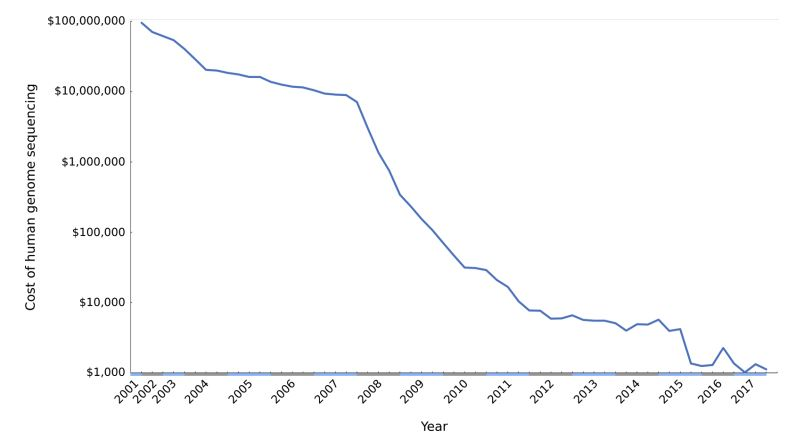
\includegraphics[width=0.7\textwidth]{fig/costPerGenome.png}
\decoRule
\caption{\textbf{Exponentially decreasing cost per Human genome, from 2009}. "\textit{Adapted from} \url{https://www.genome.gov/about-genomics/fact-sheets/Sequencing-Human-Genome-cost}"} 
\label{fig:costPerGenome}
\end{figure}

\begin{figure}[H]
\centering
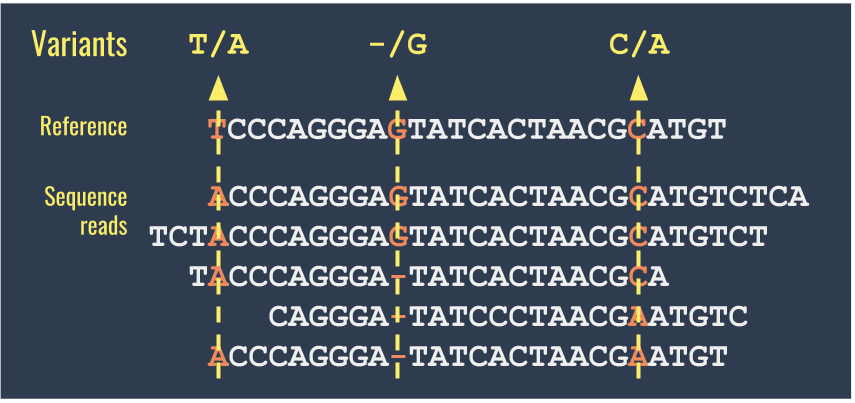
\includegraphics[width=0.7\textwidth]{fig/variantCalling.png}
\decoRule
\caption{\textbf{Variant calling} is the process of identifying genetic variants. First, sequence reads from one individual are aligned against the reference genome, then variable sites are identified as the ones where the sequence differs from the reference genome.} 
\label{fig:variantCalling}
\end{figure}

\begin{figure}[H]
\centering
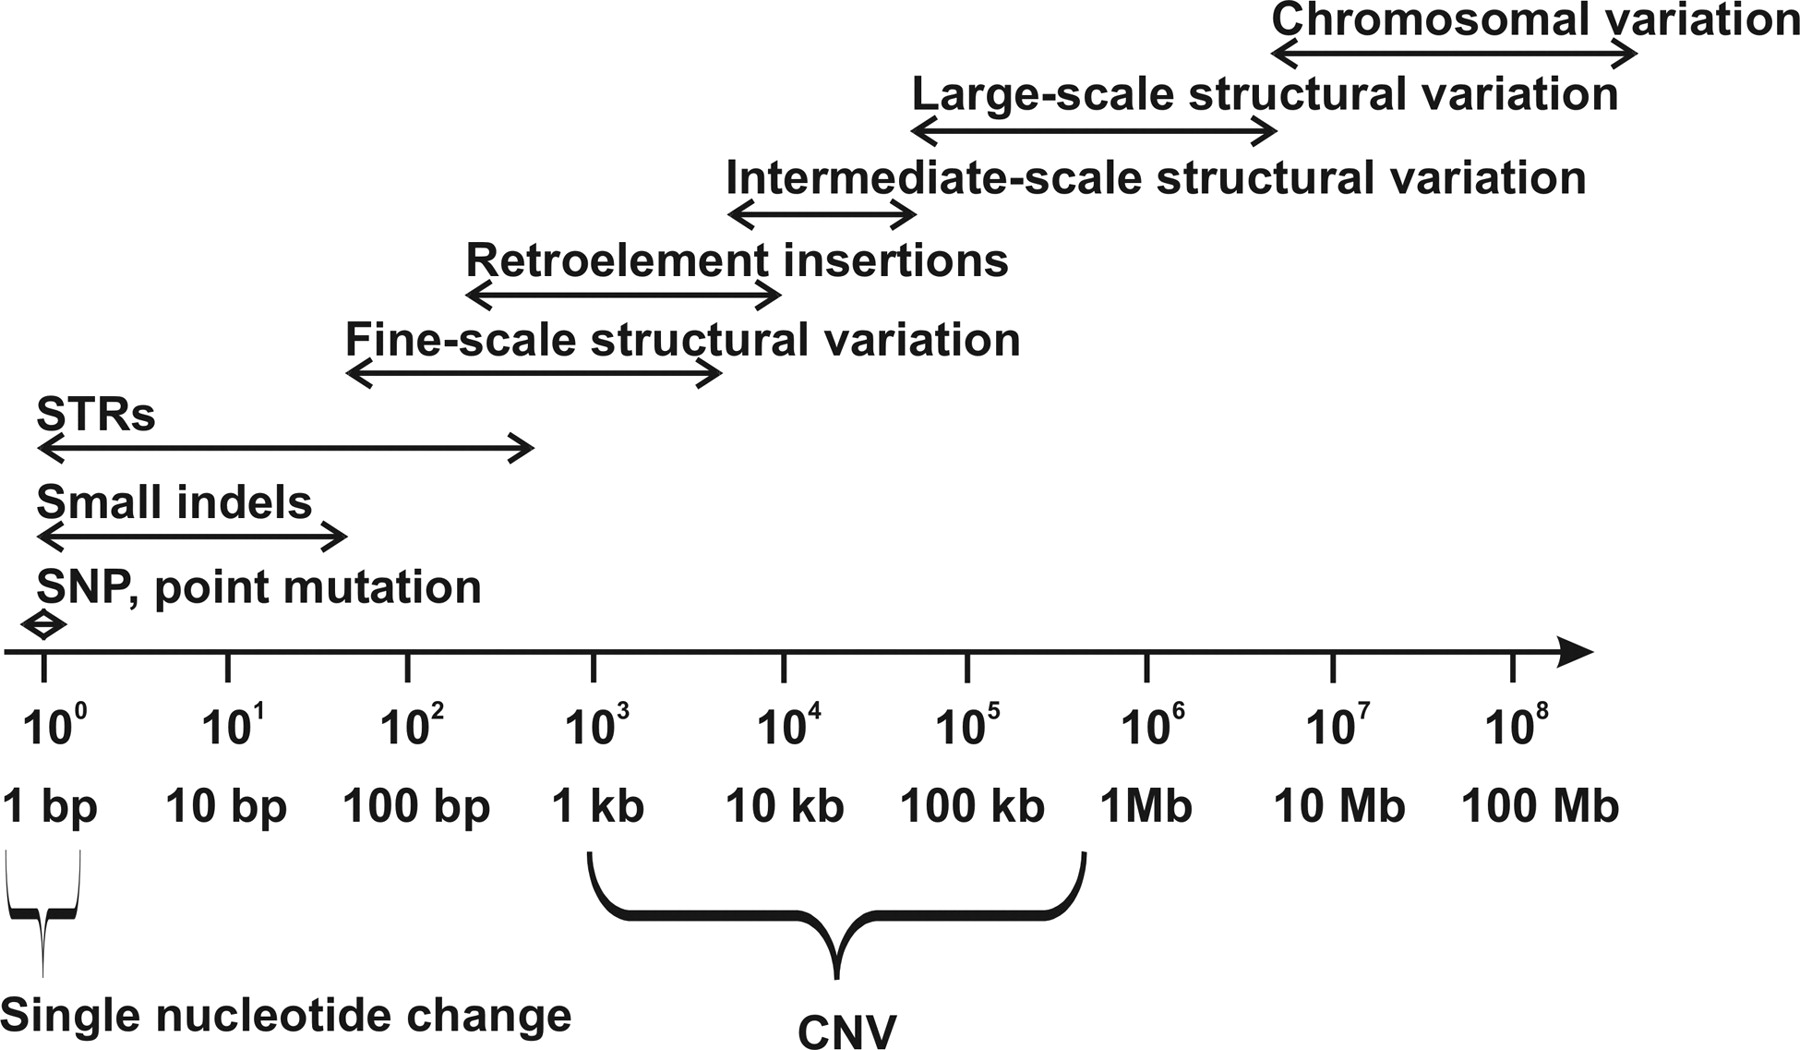
\includegraphics[width=0.7\textwidth]{fig/typeOfVariants.jpeg}
\decoRule
\caption{\textbf{Type and size of genetic variants.}"\textit{Adapted from} \cite{pollex2007copy}"} 
\label{fig:typeOfVariants}
\end{figure}

The first large-scale project that made use of whole-genome sequencing was the 1000 genomes project that used a combination of low-coverage whole-genome sequencing (WGS), deep exome sequencing, and dense microarray of 2,504 individuals from 26 populations \cite{1000genome2015global}. 
This project showed that two individuals differ at roughly  0.6\% of their genome, that corresponds at 20 millions base pairs at 4.1-5.0 million sites in a genome of 3.2 giga base (Figure \ref{fig:1000genome_grid}).\\ 

A more recent study identifies 67.3 million single-nucleotide polymorphisms (SNPs), 8.8 million small insertions or deletions (indels) and 39,997 copy number variants (CNVs) in 929 genomes. The technology used was high-coverage whole-genome sequencing (at 35X) \cite{bergstrom2019insights}. The number of variants identified by this study is comparable to the one identified by the 1000 genome project despite the lower sample size because the high-coverage sequencing increased the sensitivity. Furthermore, this study also identified 1.3 million polymorphic SNPs shared between archaic human genomes.\\

%Rare variants are more likely to derive from recent mutations, and nearly absent from genotyping array.  

%%%%%FIGURE 2.4

\begin{figure}[H]
\centering
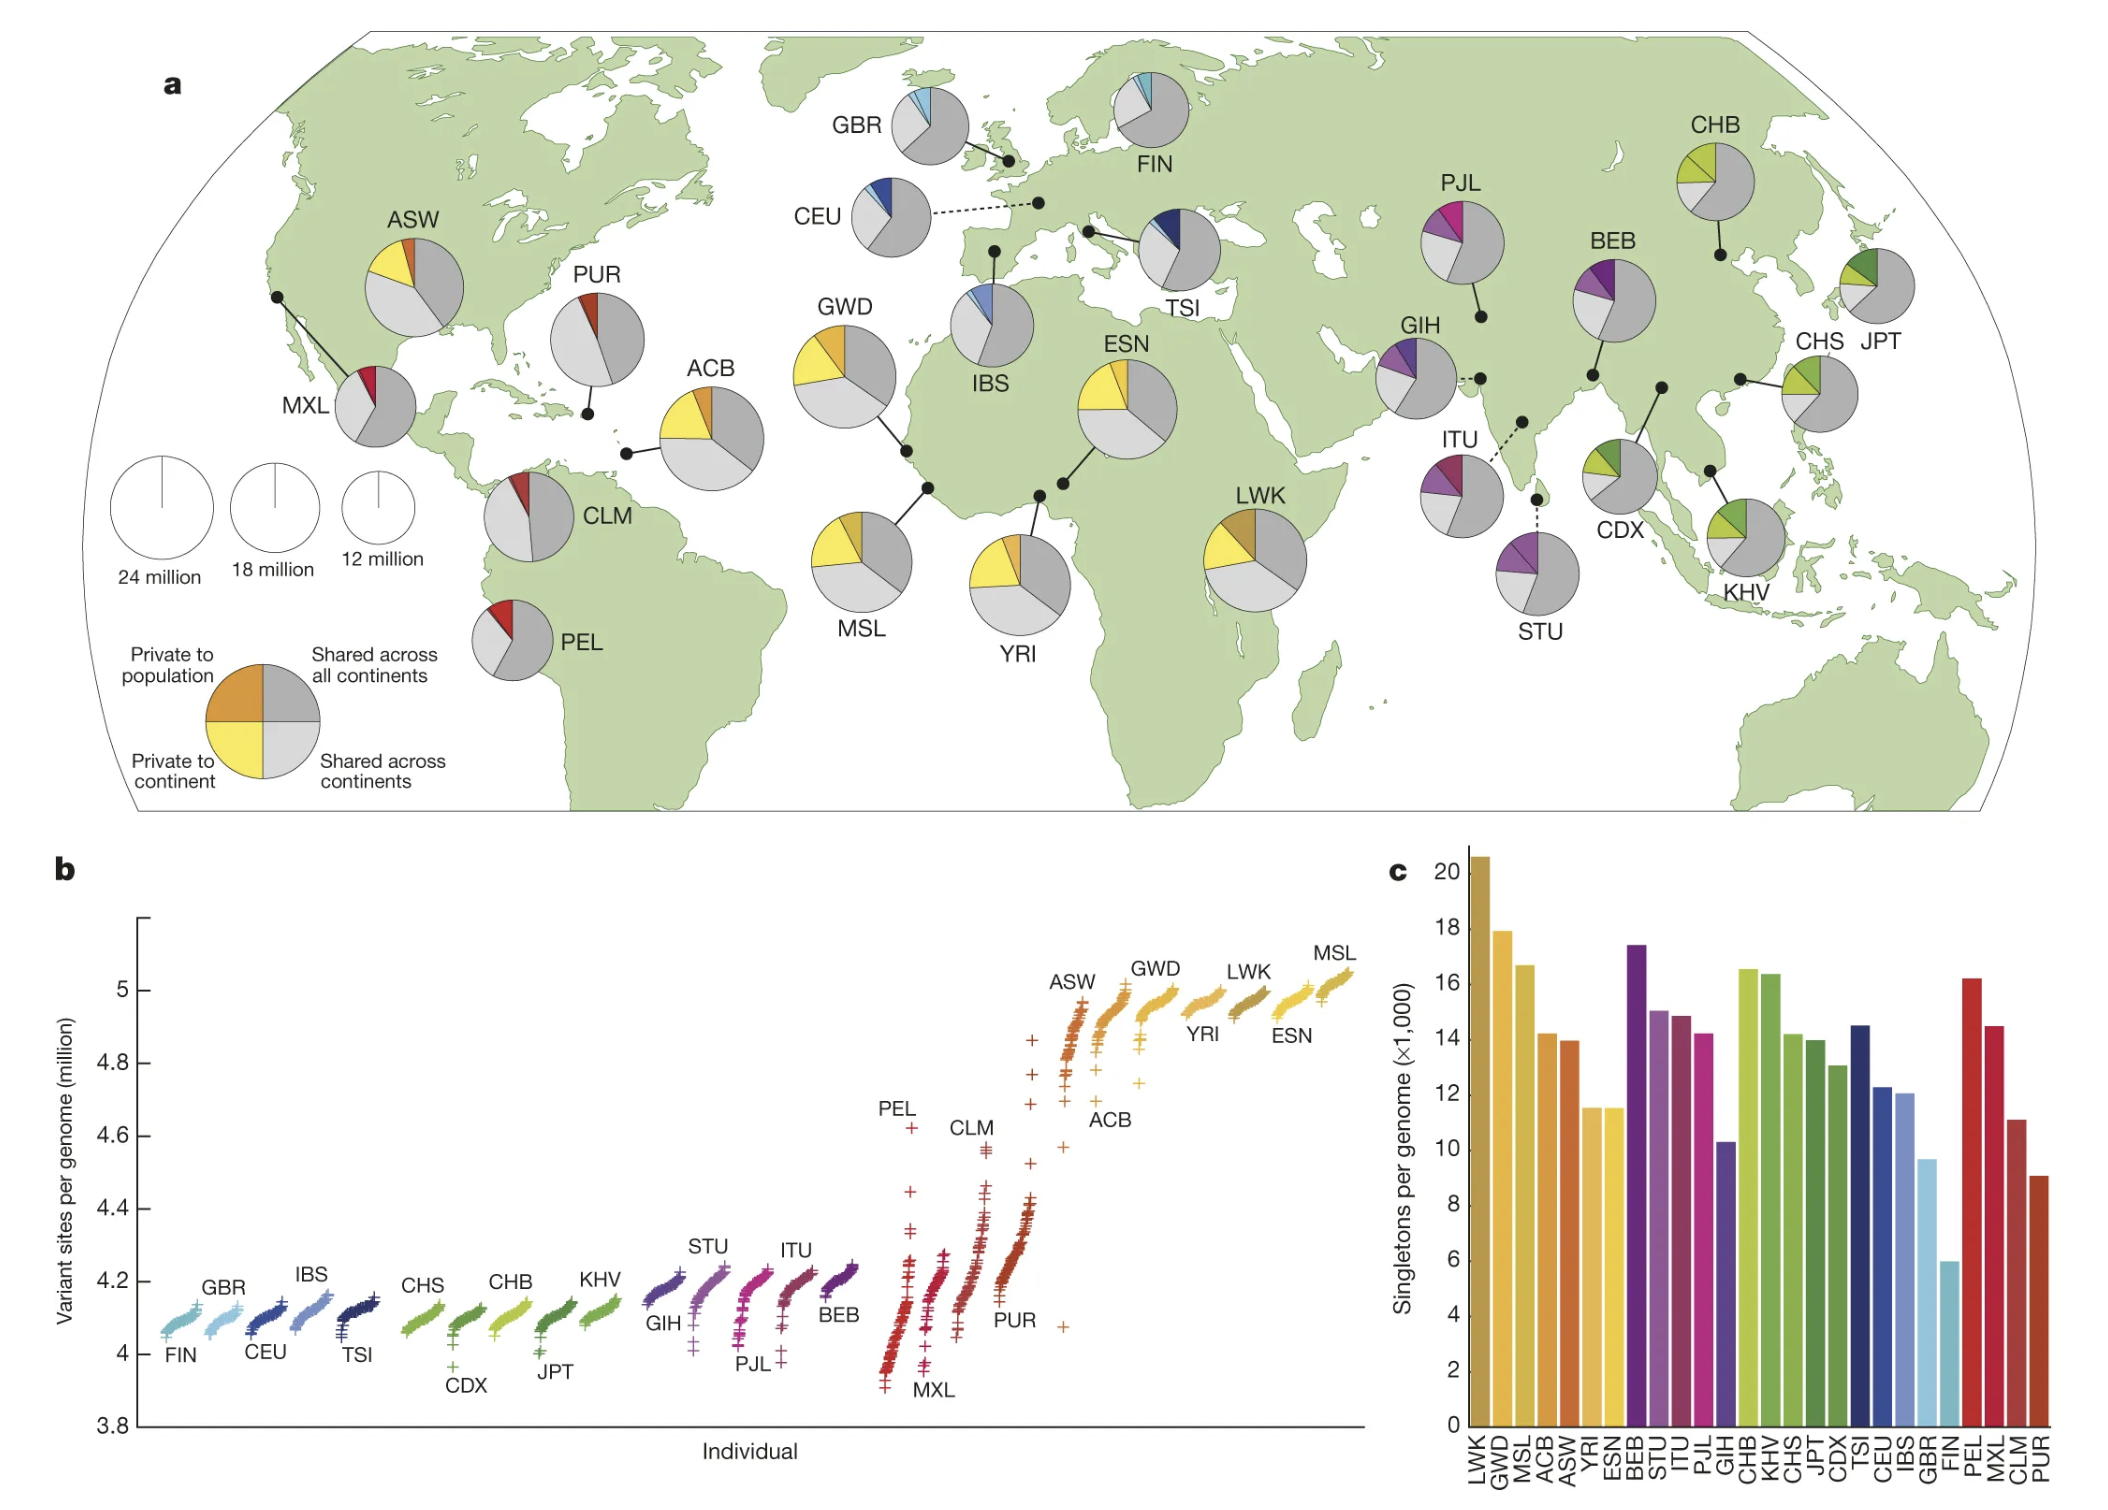
\includegraphics[width=1\textwidth]{fig/1000genome_grid.png}
\decoRule
\caption{\textbf{a}, Polymorphic variants within sampled populations. The area of each pie is proportional to the number of polymorphisms within a population. Pies are divided into four slices, representing variants private to a population (darker colour unique to population), private to a continental area (lighter colour shared across continental group), shared across continental areas (light grey), and shared across all continents (dark grey). Dashed lines indicate populations sampled outside of their ancestral continental region. \textbf{b}, The number of variant sites per genome. \textbf{c}, The average number of singletons per genome."\textit{Adapted from} \cite{1000genome2015global}}
\label{fig:1000genome_grid}
\end{figure}

%%%%%%%%%%%%%%%%%%%%%%%%%%%%%%%

\section{Genetics of miscarriages }

\subsection{Anatomy of placenta and use of the villi to extract DNA from embryos}

One week after fertilization, the blastocyst hatches from the pellucid zone and subsequently implants into the uterine wall. The placenta is a unique materno-fetal organ which begins to grow around the point of implantation and is delivered at the birth of the fetus.
The placenta has several biological functions:
\begin{itemize}
    \item \textbf{Metabolism}. The fetus takes the nutrients essential for its growth from the placenta. Some nutrients like glycogen, cholesterol, and fatty acids are synthesized in the placenta.
    \item \textbf{Transport} from and to the embryo of gases, nutrients, drugs, hormones, antibodies, wastes, and infectious agents. 
    \item \textbf{Endocrine}. After the dismission of the \textit{Corpus luteum} there is an increase of production from the placenta of human chorionic gonadotropin that is also a marker for the begin of pregnancy. Placenta also produces progesterone that helps the embryo during the implant, estrogen for proliferation and the growth of the uterus and enlargement of the breasts, human placental lactogen has structure and function similar to growth hormone and modify the metabolism of the mother to facilitate the energy supply to the fetus.
\end{itemize}

The placenta is composed of four layers that separate maternal and fetal blood \cite{placenta}:
\begin{itemize}
    \item \textbf{Syncitiotrophoblast} is the outer layer of the trophoblast and is essential for the first stage in the uterine wall invasion and homing and also establishing an interface between maternal blood and embryo. 
    \item \textbf{Cytotrophoblast} is the inner layer of the trophoblast between Syncitiotrophoblast and the external wall of the blastocyst. Contains trophoblastic stem cell. 
    \item \textbf{Villi connective tissue} is involved in the invasion of the uterine decidua and at the same time is essential to absorb nutrients from the mother for the growth of the embryo.   
    \item \textbf{Fetal capillary endothelium} is the last layer across which all exchange of gases, nutrients, hormones, and wastes occurs.
\end{itemize}

The villi are the part of the placenta that was used to extract the DNA \cite{you2008multiple} for sequencing in this project. 


\subsection{Known genetic causes of miscarriages}
%~~~~~~~~~~~~~~~ definizione 
Human reproduction is highly ineffective and it is estimated that 10-20\% of all pregnancies end in early miscarriage or early pregnancy loss (PL) during the first trimester \cite{goddijn2000genetic,zhang2009genetic} and up to 50\% of cases of recurrent pregnancy loss (RPL) do not have a clearly defined etiology \cite{practice2012evaluation}. Miscarriage is defined as the death of the fetus within 20-28 week of gestation \cite{pmid27994187, pmid25055407, pmid25944391, pmid11821293, stephenson2002cytogenetic, pmid25681385, pmid29858908}. RPL is defined as the loss of two or more consecutive pregnancies\cite{green2019review}. 
%~~~~~~~~~~~~~~~~~ consequenze aborto nella madre 
The loss of the fetus can cause physical and psychological complications to the mother, such as infection or bleeding, anxiety, guilt, and sadness. \cite{robinson2014pregnancy}.\\ 

%~~~~~~~~~~~~~~~~ cause
Miscarriages can occur for medicals or genetics causes. The most common medicals causes are infection or maternal pathology as diabetes, hypothyroidism or uterine anatomical abnormalities \cite{najafi2019chromosomal}. Mother age is an actual risk but also parental age is a risk factor in couples composed of a woman aged ≥35 years and man aged ≥40 years \cite{de2002paternal}, lifestyle is also important for pregnancy and exposure to tobacco, smoke, drug or alcohol use can be a risk factor for a miscarriage \cite{andersen2014risk}.\\

Among the genetic causes, the most common are chromosomal aneuploidies such as trisomies or deletions of large chromosomal chunks \cite{goddijn2000genetic,zhang2009genetic}. In humans, aneuploidy is the most common cause of miscarriage and can occur during mitosis in the oocytes or in sperms. The rate of aneuploidies is higher in humans (5-20\% of oocytes) than in other species (1/10,000 meiotic yeast cells, 1/2000-1/6000 Drosophila germ cells, and 1/100-1/200 murine germ cells) \cite{niakan2012human}.
Currently, it is possible to screen for aneuploidies with two methods, both invasive, chorionic villus sampling (CVS) and amniocentesis. The CVS can be made from 10 through 13 weeks’ gestation and amniocentesis is performed starting at 15 weeks’ gestation. The associated risks for a miscarriage with these two procedures are 3\% for CVS and 0.8\% for amniocentesis \cite{caughey2006chorionic}.\\

Screening for aneuploidies or other chromosomal aberration is routine prior to \textit{in vitro} fertilisation \cite{driscoll2008first}. When it is done on a miscarried fetus on DNA extracted from chorionic villi, 50-60\% of RPL cases present aneuploidies while in the remaining 40-50\% the causes are unknown \cite{pmid27994187, pmid25944391, pmid11821293, stephenson2002cytogenetic, pmid22796359, pmid22672580, pmid25681385, gaboon2013recurrent, pmid30642578}.\\


\subsection{Current knowledge of the genetic studies on miscarriages}
%~~~~~~~
The first large-scale study of miscarriage is from 2019 and was a genome-wide association study (GWAS) done on 69,118 cases from five different ancestries (trans-ethnic) for sporadic miscarriage, 750 cases of European ancestry for recurrent miscarriage, and 359,469 female has negative control \cite{laisk2019genetic}. This study identified one genome-wide significant association on chromosome 13 (rs146350366, minor allele frequency, MAF=1.2\%) for sporadic miscarriage in \textit{FGF9} responsible for the maintenance of the pregnancy and progesterone production; three genome-wide significant associations for recurrent miscarriage in chromosome 9 (rs7859844, MAF=6.4\%) chromosome 11 (rs143445068, MAF=0.8\%) and chromosome 21 (rs183453668, MAF=0.5\%). While notable for the size of the sample, this study has two main limitations. First, it is carried out on the mothers, therefore it seeks half of the possible cause of the miscarriage. Secondly, it was done using 8,664,066 markers, therefore ignoring a very large fraction of the genome. \\

Next-generation sequencing (NGS) is already used to identify mutations in fetuses with anomalies detected by ultrasound technology but is still not largely used in the study of the genetic causes of pregnancy loss. NGS is the best choice to have an adequate resolution in genetic studies. In fact, the expectation is that miscarriages depend not on a single mutation but on a combination of mutations such as compound heterozygosis \cite{qiao2016whole}. Linkage analysis on whole-exome sequences (WES) of miscarriages in two families identifies a compound heterozygous variants in \textit{DYNC2H1} (MIM 603297) at chromosome 11q22.3 in the first exon. The second family presenting two miscarriages had mutations in \textit{ALOX15} (rs113604586, rs34210653) with a minor allele frequency for all variants <1\%.\\

A recent study on 19 cases of missed abortion, uses another strategy that is filtering based on a list of 286 genes associated with early embryonic lethality and missed abortion provided by \textsc{geneontology} (GO, chordate embryonic development, cell proliferation, and forebrain development) \cite{fu2018whole}. This study identified 36 sequence variants in 32 candidate genes.\\ 

The actual use of WES in clinical analysis for the detection of variants is limited to the coding sequence to identify changes to the protein product. The successful usage of WES is due to the fact that it probably contains most (85\%) of the genes associated with diseases, the costs of the data are lower and the size is easier to manage than whole-genome sequencing \cite{rabbani2014promise}. Nevertheless, low-coverage whole-genome sequencing has already been proved useful to identifying chromosome rearrangements and copy number variants (CNVs) \cite{rajcan2019next} and it is probably the most comprehensive tool for the study of the genomic variation responsible for miscarriages since it includes also regulatory and intergenic regions. \\


\section{Project GREP}
The work I have done during my thesis is part of the project \textit{Genomics of REcurrent Pregnancy loss (GREP)} lead by the Institute of Genetics and Biophysics of the National Research Council in collaboration with the University of Napoli Federico II, and several other partners in Italy, United Kingdom, Malaysia, Pakistan, and Australia.  

GREP aims to identify genetic variants likely to cause PL not seen by current diagnostic tools (mainly comparative genomic hybridization), either because of the size or because they are located in non-coding regions not considered in medical diagnostics. The main objective of GREP is to build a predictive model that integrates genomic variation and functional annotations, based on the analysis of whole-genome sequences of miscarried embryos.\\

I participate in the data analyses of the GREP pilot project (Figure \ref{fig:projectPhases}) that includes four main stages. The first step was the collection of samples done by the University of Ferrara during 2016-2018, followed by a step of screening for euploid samples to be sequenced. Sequenced samples are being analyzed and the results will be validated using a biobank of embryonic DNA and eventually cellular models. More details will be outlined in the Result section. 

\begin{figure}[H]
\centering
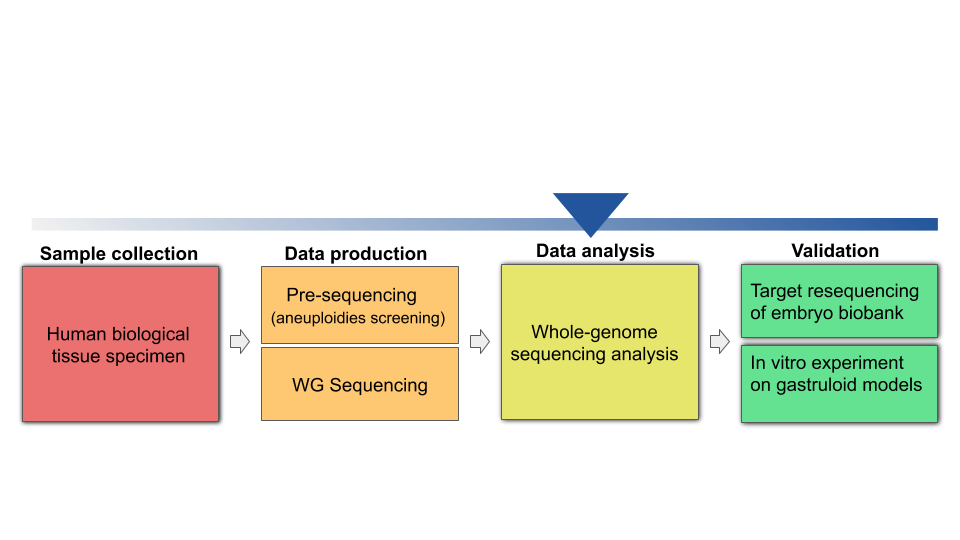
\includegraphics[width=0.80\textwidth]{fig/projectPhases.png}
\decoRule
\caption{\textbf{Pilot project phases.}} 
\label{fig:projectPhases}
\end{figure}




% Chapter discussion

\chapter{Aim of the study} % Main chapter title

\label{Chapter2} % For referencing the chapter elsewhere, use \ref{Chapter4} 

%----------------------------------------------------------------------------------------

% Define some commands to keep the formatting separated from the content 
\newcommand{\keyword}[1]{\textbf{#1}}
\newcommand{\tabhead}[1]{\textbf{#1}}
\newcommand{\code}[1]{\texttt{#1}}
\newcommand{\file}[1]{\texttt{\bfseries#1}}
\newcommand{\option}[1]{\texttt{\itshape#1}}

%~~~~~~~~~~~~~~~~~~~~~~~~~~~~~~~~~~~~~~~~~~~~~~~~~~~~~~~~~~~~~~~~~~~~~~~~~~~~~~~~~~~~~~~

%~~~~ aim:
The aim of this study is to identify genomic variants likely to cause idiopathic pregnancy losses that are not seen by current diagnostic tools either because of their very small size or because they lie in non-coding regulatory regions of the genome that are not routinely sequenced.

The expectation is to identify highly deleterious dominant \textit{de novo} mutations in sporadic cases and rare moderately deleterious recessive mutations in homozygosis or compound heterozygosity in recurrent pregnancy losses (Figure \ref{fig:expectation}).\\

%~~~~ objectives: 
The objectives were to: 

- analyze whole-genome sequencing data to assemble human sequences obtained by sequencing of miscarried embryos and identify genomic variants

- develop a pipeline to prioritize genetic variants based on their putative deleteriousness  

- identify diagnostic mutations\\

%~~~~ novelties: 
There are two main novelties in this study. First, compared to previous studies, it investigates the genome of the embryos rather than those of parents. Secondly, it uses a whole-genome approach, through high-coverage (30X) whole-genome sequencing allowing to investigate not only genic regions but also regulatory and intergenic ones.

\begin{figure}[H]
\centering
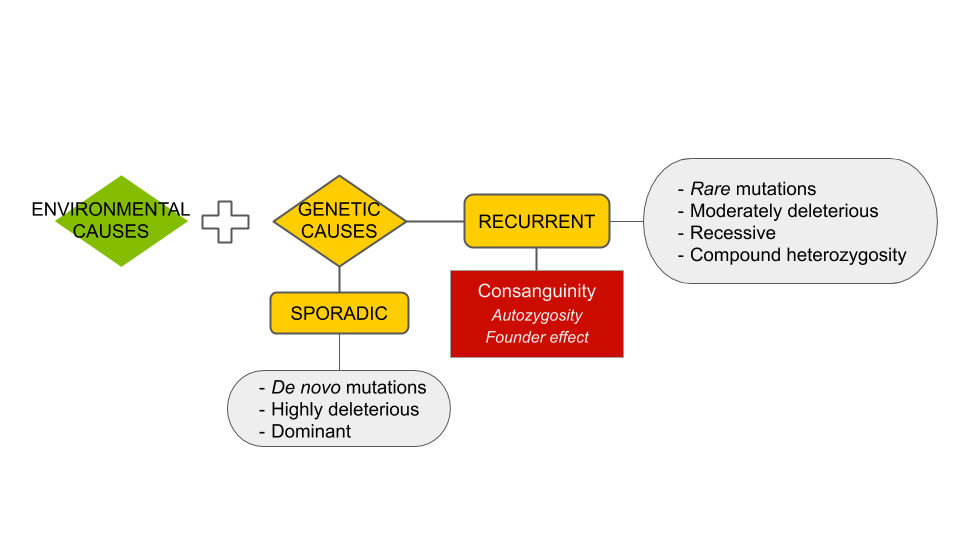
\includegraphics[width=0.90\textwidth]{fig/expectation.png}
\decoRule
\caption{\textbf{Genetic model behind miscarriages.} Expectations on types and frequencies of mutations.} 
\label{fig:expectation}
\end{figure}

% Chapter results

\chapter{Results} % Main chapter title

\label{Chapter3} % For referencing the chapter elsewhere, use \ref{Chapter3} 

%----------------------------------------------------------------------------------------

% Define some commands to keep the formatting separated from the content 
\newcommand{\keyword}[1]{\textbf{#1}}
\newcommand{\tabhead}[1]{\textbf{#1}}
\newcommand{\code}[1]{\texttt{#1}}
\newcommand{\file}[1]{\texttt{\bfseries#1}}
\newcommand{\option}[1]{\texttt{\itshape#1}}

%~~~~~~~~~~~~~~~~~~~~~~~~~~~~~~~~~~~~~~~~~~~~~~~~~~~~~~~~~~~~~~~~~~~~~~~~~~~~~~~~~~~~~~~


%%%%%%%%%%%%%%%%%%%%%%%%%%%%%%%%%%%%%%%%%%%%%%%%%%%%%%%%%%%%%%%%%%%%%%%%%%%%%%%%%%%%%%%
%  Section 
%%%%%%%%%%%%%%%%%%%%%%%%%%%%%%%%%%%%%%%%%%%%%%%%%%%%%%%%%%%%%%%%%%%%%%%%%%%%%%%%%%%%%%%


\section{Description of the data set}
Data consists of a database of medical records from interviews of 45 recurrent pregnancy loss (RPL), 74 first pregnancy loss (FPL), and 131 Voluntary Termination of pregnancy (VTP) with no previous miscarriages. The large majority of cases is of European origin (82.7\%, African 9.6\%, Asian 7.6\%).\newline

Data was stored in Excel format that is not suitable for streamed bioinformatics analyses. Therefore, my first task was to format the files and control for errors generated when the table was manually written, \textit{e.g.} typos or white spaces. To do so, I used the open-source software Open Refine \cite{openRefine} that cleans and adjusts data formatting. This process generates a refined database of the original table suitable for bioinformatics preliminary analysis to explore properties of the data. As an example, it is possible to known  if a medical condition is the cause of the PL and exclude this sample from further genetic analyses.\\

Using the refined database I did a first exploratory analysis that consists on graphical representation of data.  The gestational age at pregnancy termination (Figure \ref{fig:panel_edu_gestAge_mothAge}.B, Mann-Whitney p-value\textsubscript{ FPL-RPL}= 0.250, p-value\textsubscript{ VTP-FPL}= 0.003, p-value\textsubscript{ VTP-RPL}= 0.002 ) is comparable between VTP, FPL, and RPL, though the VTP falls in these intervals because the legal term for voluntary termination of pregnancy is twelve weeks. We observed a trend of higher incidence of RPL in women with high education, (Figure \ref{fig:panel_edu_gestAge_mothAge}.A), most likely because the age of pregnancy tend to be higher than other women for social reasons. 

\begin{figure}[H]
\centering
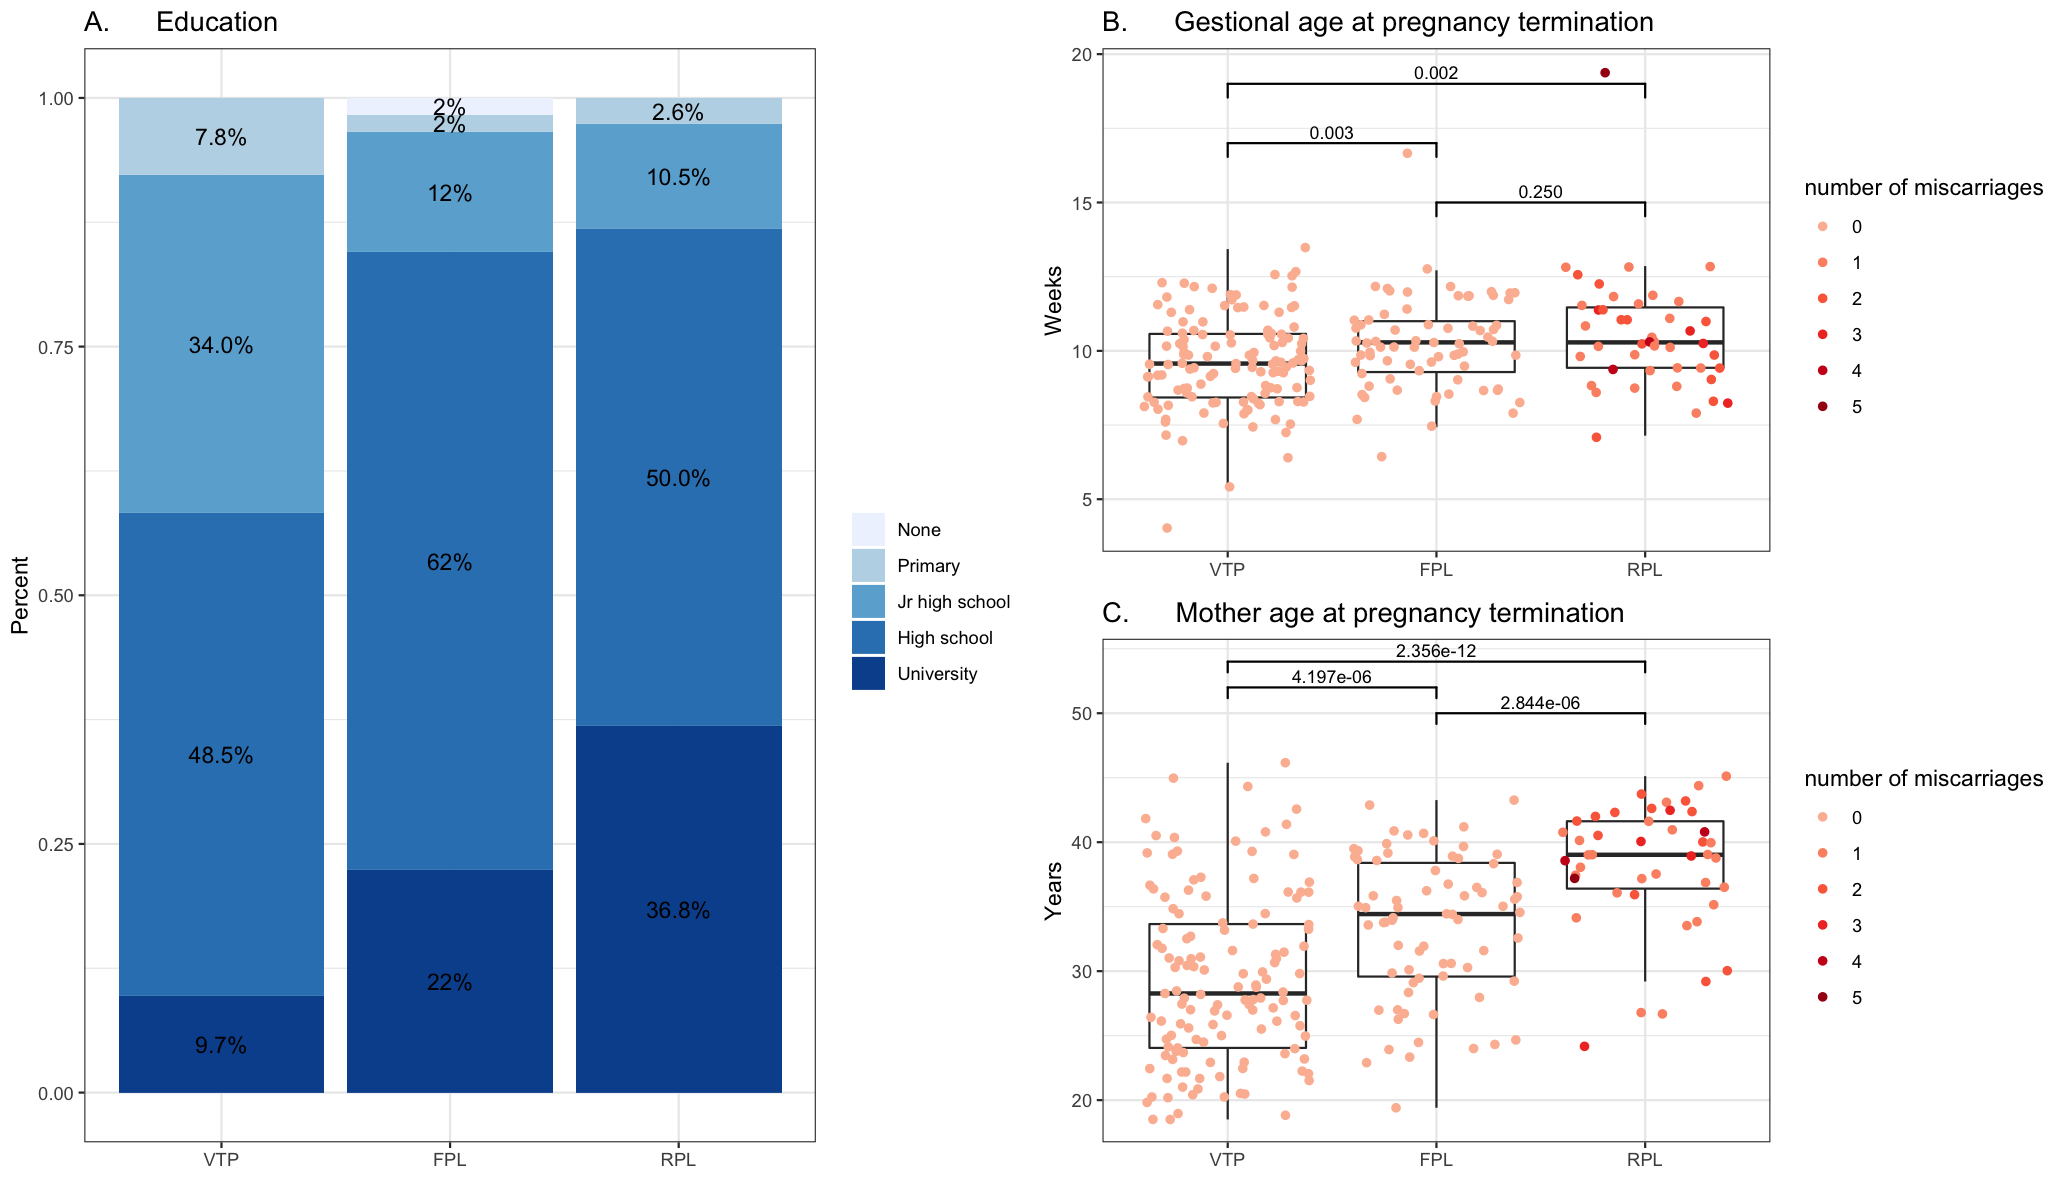
\includegraphics[width=1.10\textwidth]{fig/panel_edu_gestAge_mothAge.png}
\decoRule
\caption{\textbf{Fig A: Education.} RPL samples tend to have higher educational level compared to VTP, probably due high age at first pregnancy of educated woman. \textbf{Fig B:Gestational age at pregnancy termination.} The age of the embryo in PLs range from 4 to 19.4 weeks and there are no significant differences between pairs of classes. \textbf{Fig C: Age of the mother.} Median age of the mother at the event is significantly higher
in RPL compared to FPL.}
\label{fig:panel_edu_gestAge_mothAge}
\end{figure}



Consistently, the median mother age at pregnancy termination is higher in RPL compared to FPL, suggesting that recurrent miscarriages happen more often at advanced age (Figure \ref{fig:panel_edu_gestAge_mothAge}.C, Mann-Whitney p-value\textsubscript{ FPL-RPL}= 2.84e10\textsuperscript{6}). Moving medical parameters, we see no significant differences between RPL, FPL and VTP in terms of Body Mass Index (Figure \ref{fig:panel_BMI_MenAge}.B, Mann-Whitney p-value\textsubscript{ FPL-RPL}= 0.675, p-value\textsubscript{ VTP-FPL}= 0.485, p-value\textsubscript{ VTP-RPL}= 0.620 ), while we observe a wider range of the age at menarche in RPL (8-17 years old) compared to FPL and VTP (Figure \ref{fig:panel_BMI_MenAge}.A, F-test p-value\textsubscript{ VTP-RPL}= 0.0016, p-value\textsubscript{ FPL-RPL}= 0.0288 ).  \newline



\begin{figure}[H]
\centering
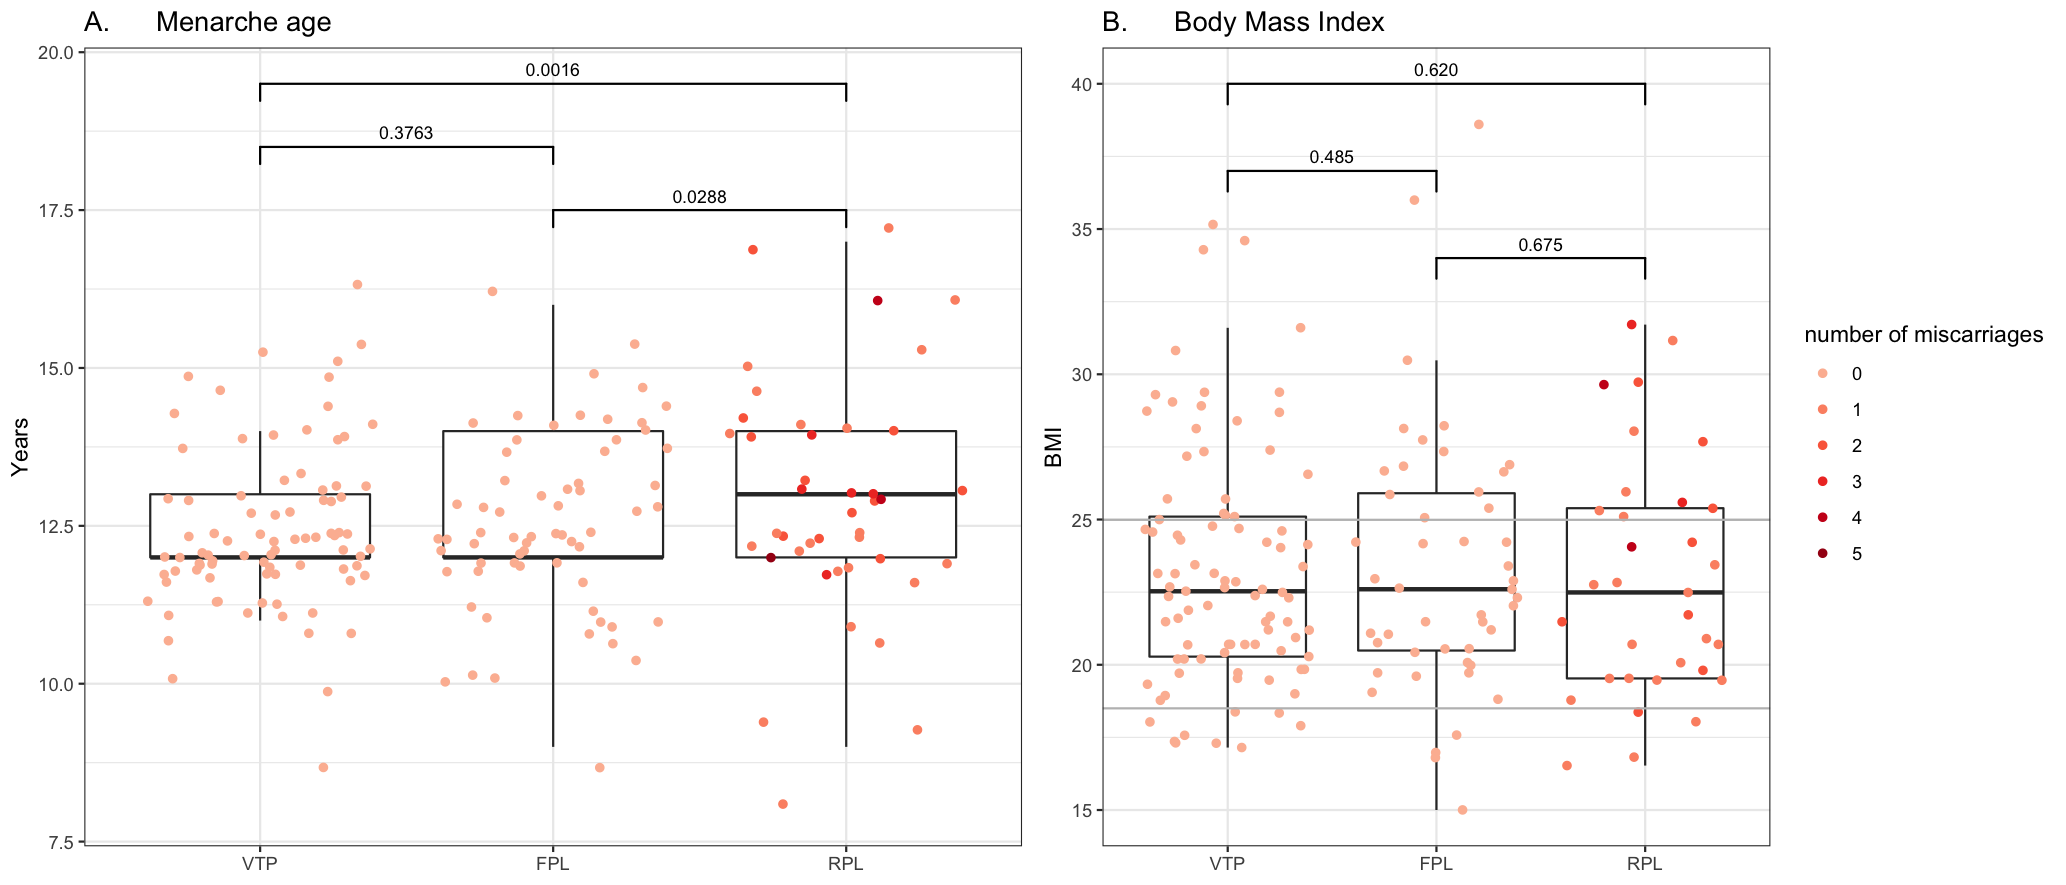
\includegraphics[width=1.15\textwidth]{fig/panel_BMI_MenAge.png}
\decoRule
\caption{\textbf{Fig A:} Age of the menarche is significantly wider in RPL compared to FPL and VTP. \textbf{Fig B:} BMI does not influence pregnancy loss compared to VTP.}
\label{fig:panel_BMI_MenAge}
\end{figure}


%Overall we demonstrate that our data set complies to the standard.. DIsCUSSION 

%%%%%%%%%%%%%%%%%%%%%%%%%%%%%%%%%%%%%%%%%%%%%%%%%%%%%%%%%%%%%%%%%%%%%%%%%%%%%%%%%%%%%%%%%%%%%
%  Section 
%%%%%%%%%%%%%%%%%%%%%%%%%%%%%%%%%%%%%%%%%%%%%%%%%%%%%%%%%%%%%%%%%%%%%%%%%%%%%%%%%%%%%%%%%%%%%

\section{Identification of euploid samples for genetic analyses}
In half of the pregnancies in the first trimester, the causes of PL are large chromosomal aneuploidies, such as trisomies or deletions of large chromosomal chunks \cite{goddijn2000genetic,zhang2009genetic}. With this project, we want to focus on cases in which the embryo is euploid when analyzed with current diagnostic techniques i.e. comparative genomic hybridization (arrayCGH). Hence, samples were screened for chromosomal aneuploidies prior to whole-genome sequencing. This task was performed before my thesis work started, nevertheless, I am describing it here because of its importance. \\

In 44 samples when screened for maternal contamination 11.4\% drops off the analysis, due to technical challenges during sample collection. The first round of detection of aneuploidies on chromosomes 13, 15, 16, 18, 21, 22, X, and Y through Short Tandem Repeats analysis discarded 47.7\% of samples. These types of repeats (tetra- or penta-nucleotide) are often expected to be found in heterozygosis, therefore triploidy is assumed when three alleles are found at several markers along a chromosome (complete) or part of it (partial). Similarly, uniparental disomy for a targeted region or chromosome is assumed when only one parental allele is amplified. Subsequent analysis through array-CGH and \gls{copy number variation} detection form low-coverage sequencing discarded another 11.4\% of samples (Figure \ref{fig:pipelineOutcome}).

The most common aneuploidy in our data set is the trisomy of chromosome 22 (15.9\%), followed by trisomy of chromosome 16 (9\%)(Figure \ref{fig:preseqOutcome}).\newline

Overall 29.5\% of samples were euploid (Figure \ref{fig:preseqOutcome}) and could proceed to whole-genome sequence analysis. By the time I started my thesis I had access to six samples for which sequence data was ready and available to be sequenced. 

\begin{figure}[H]
\centering
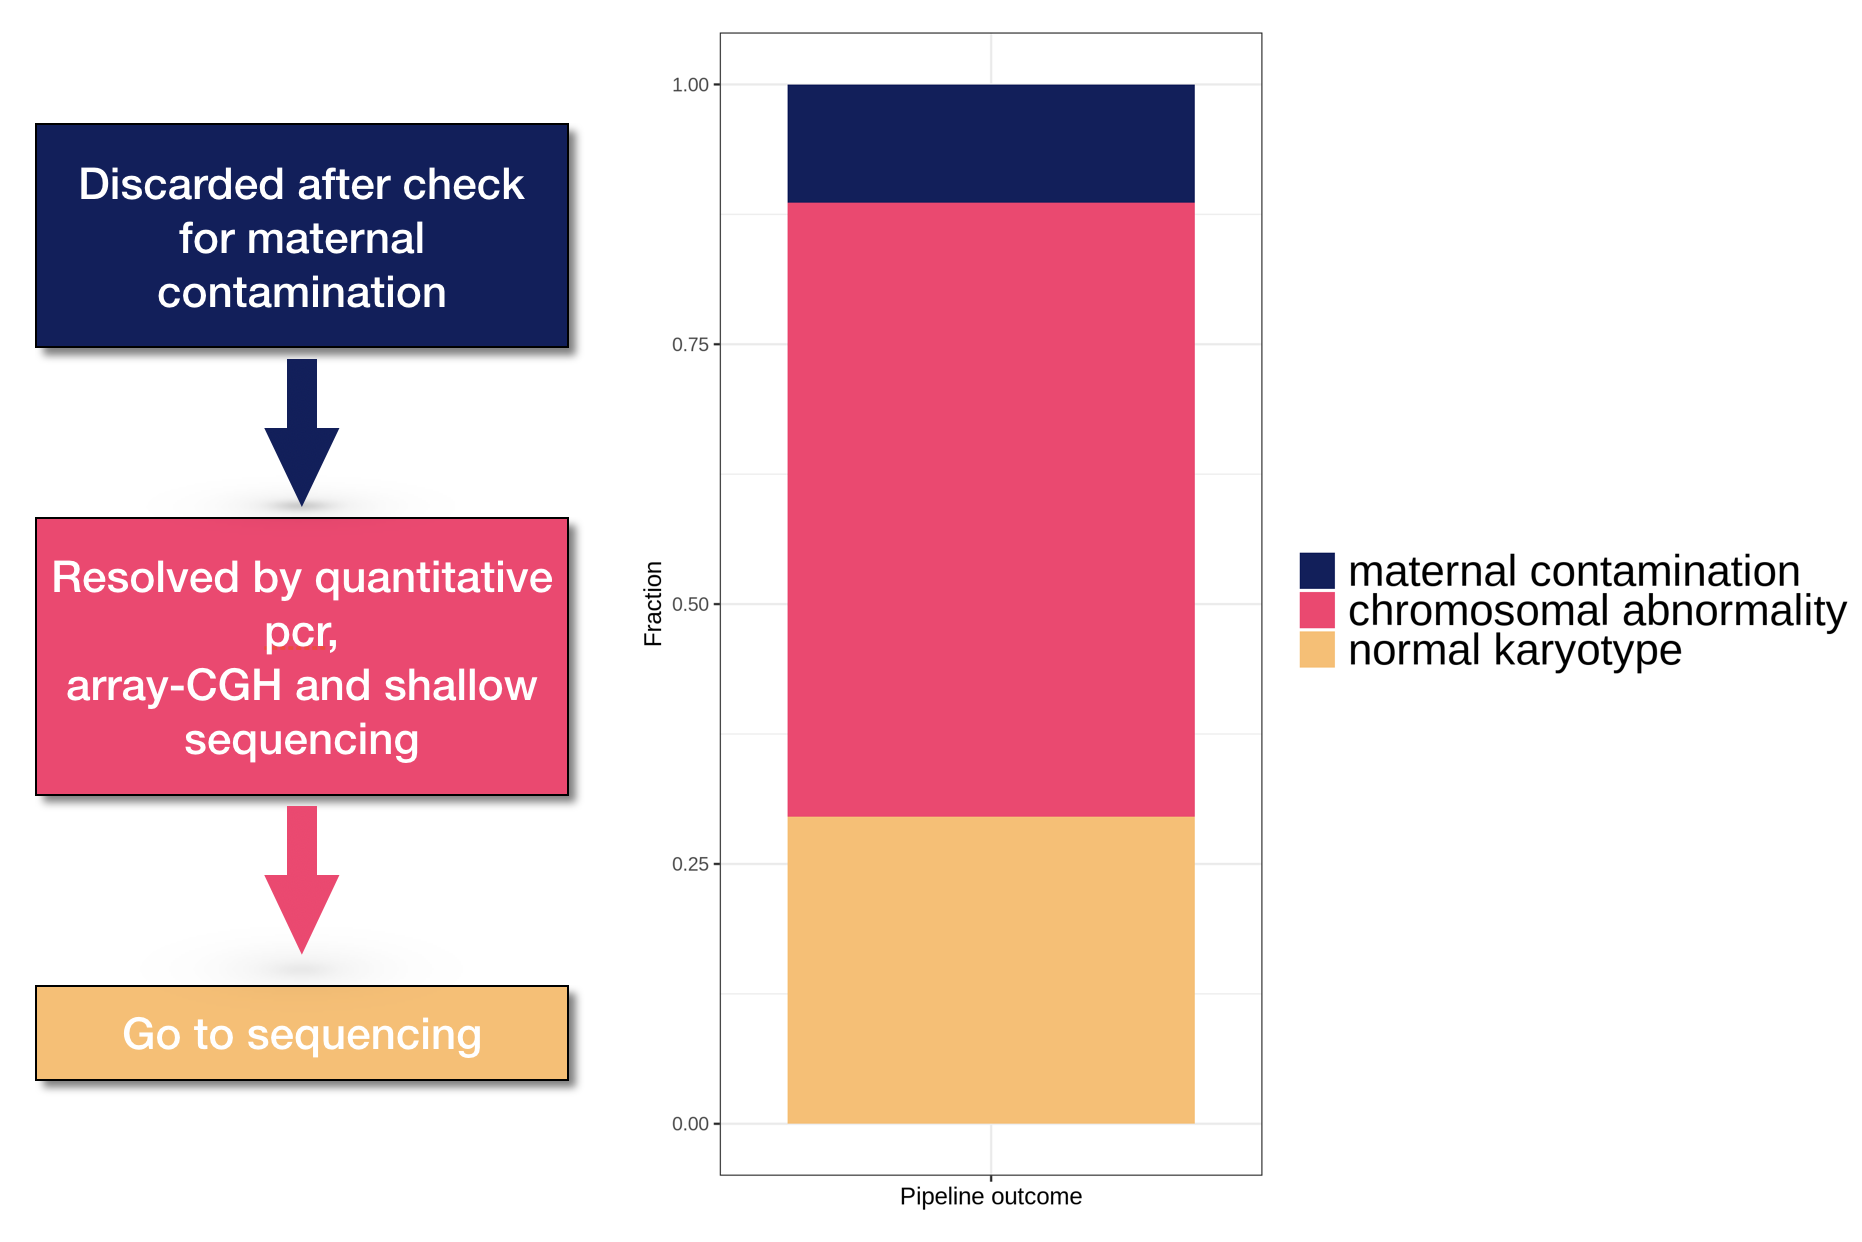
\includegraphics[width=0.7\textwidth]{fig/sampletocollectG.png}
\decoRule
\caption{\textbf{Pre-sequencing screening outcome.} Approximately 10\% of samples are discarded due to maternal contamination, and 60\% for aneuploidies. Finally ~30\% of cases are euploid and proceed to sequencing.}
\label{fig:pipelineOutcome}
\end{figure}

\begin{figure}[H]
\centering
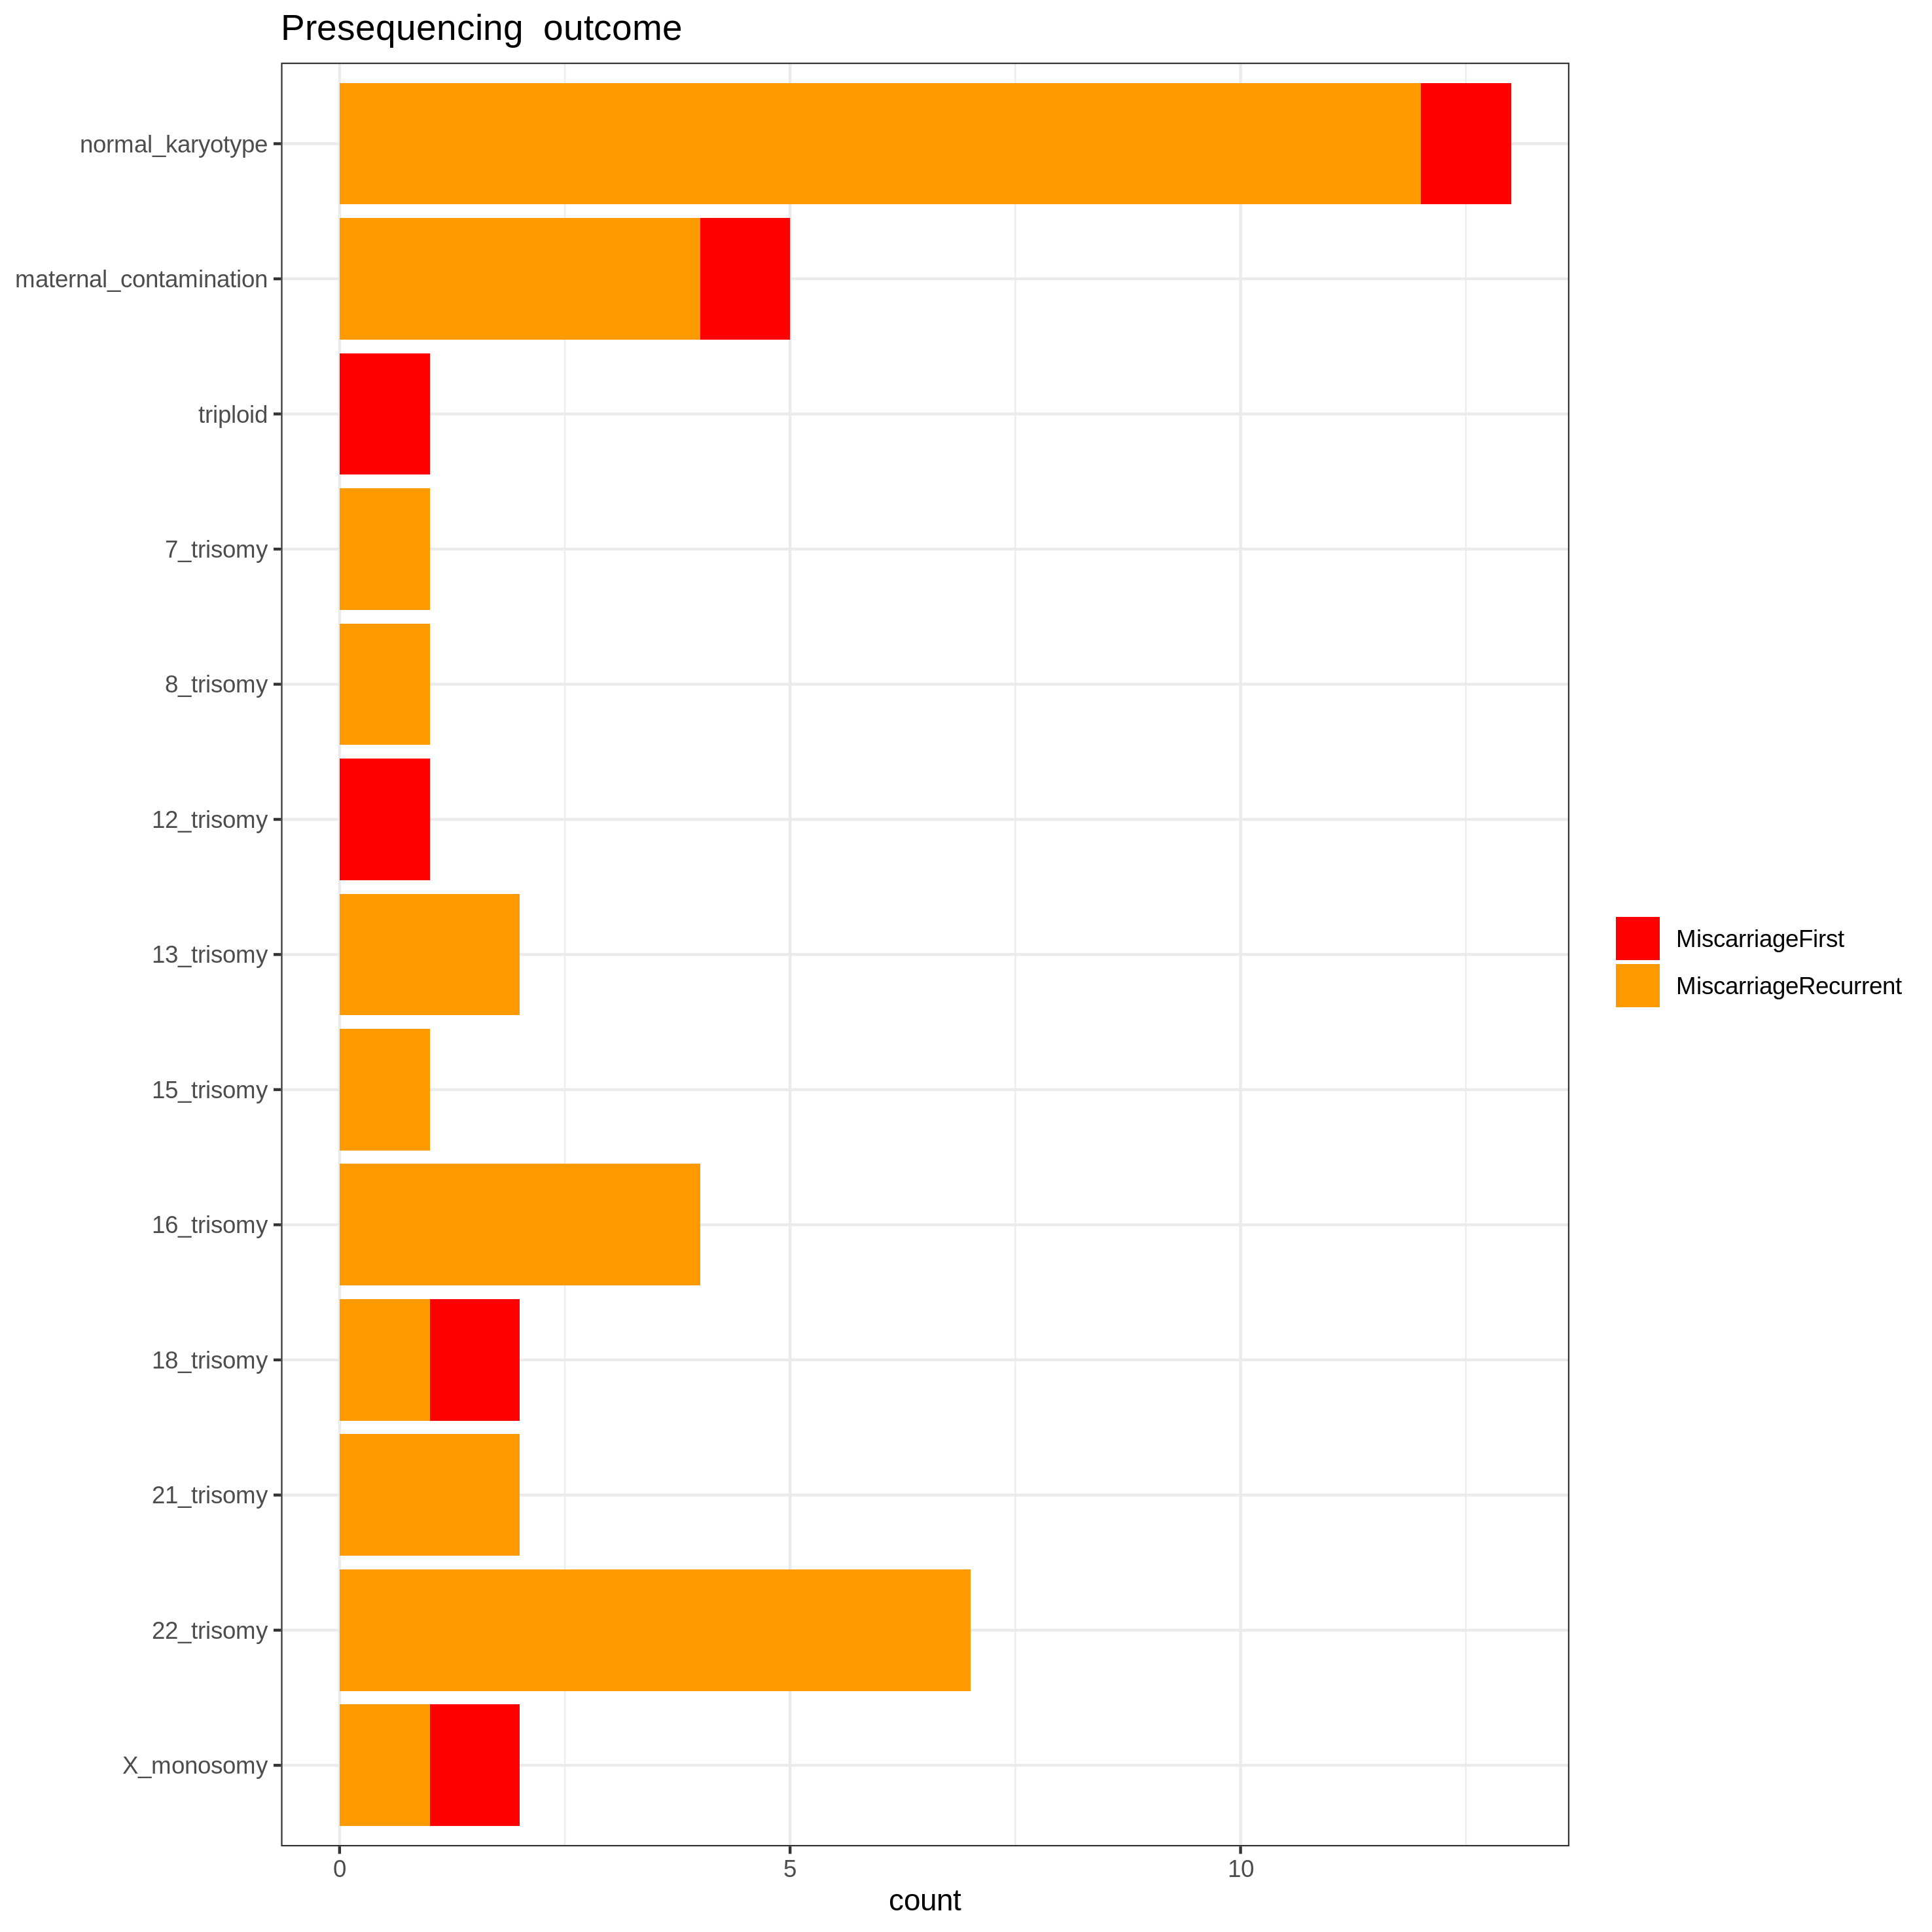
\includegraphics[width=0.8\textwidth]{fig/preseqOutcome.png}
\decoRule
\caption{\textbf{Chromosomal aneuploidies detected in the embryos.} The most common aneuploidies are trisomy on chromosome 22 followed by trisomy on chromosome 16.}
\label{fig:preseqOutcome}
\end{figure}


%%%%%%%%%%%%%%%%%%%%%%%%%%%%%%%%%%%%%%%%%%%%%%%%%%%%%%%%%%%%%%%%%%%%%%%%%%%%%%%%%%%%%%%%%%
%  Section 
%%%%%%%%%%%%%%%%%%%%%%%%%%%%%%%%%%%%%%%%%%%%%%%%%%%%%%%%%%%%%%%%%%%%%%%%%%%%%%%%%%%%%%%%%%

\section{Analysis of whole-genome sequence of embryos from pregnancy loss}
\subsection{Pipeline for the identification of genetic variants}
The sequencing pipeline produces sequence data in the \gls{fastq} format that constitutes the raw sequence data and can be used to perform the analysis from scratch and customized pipelines on \gls{high performance computing} machines. Figure \ref{fig:align-ref-vc} provides an overview of the pipeline used in this study.\newline

\vspace{1cm}

\begin{figure}[H]
\centering
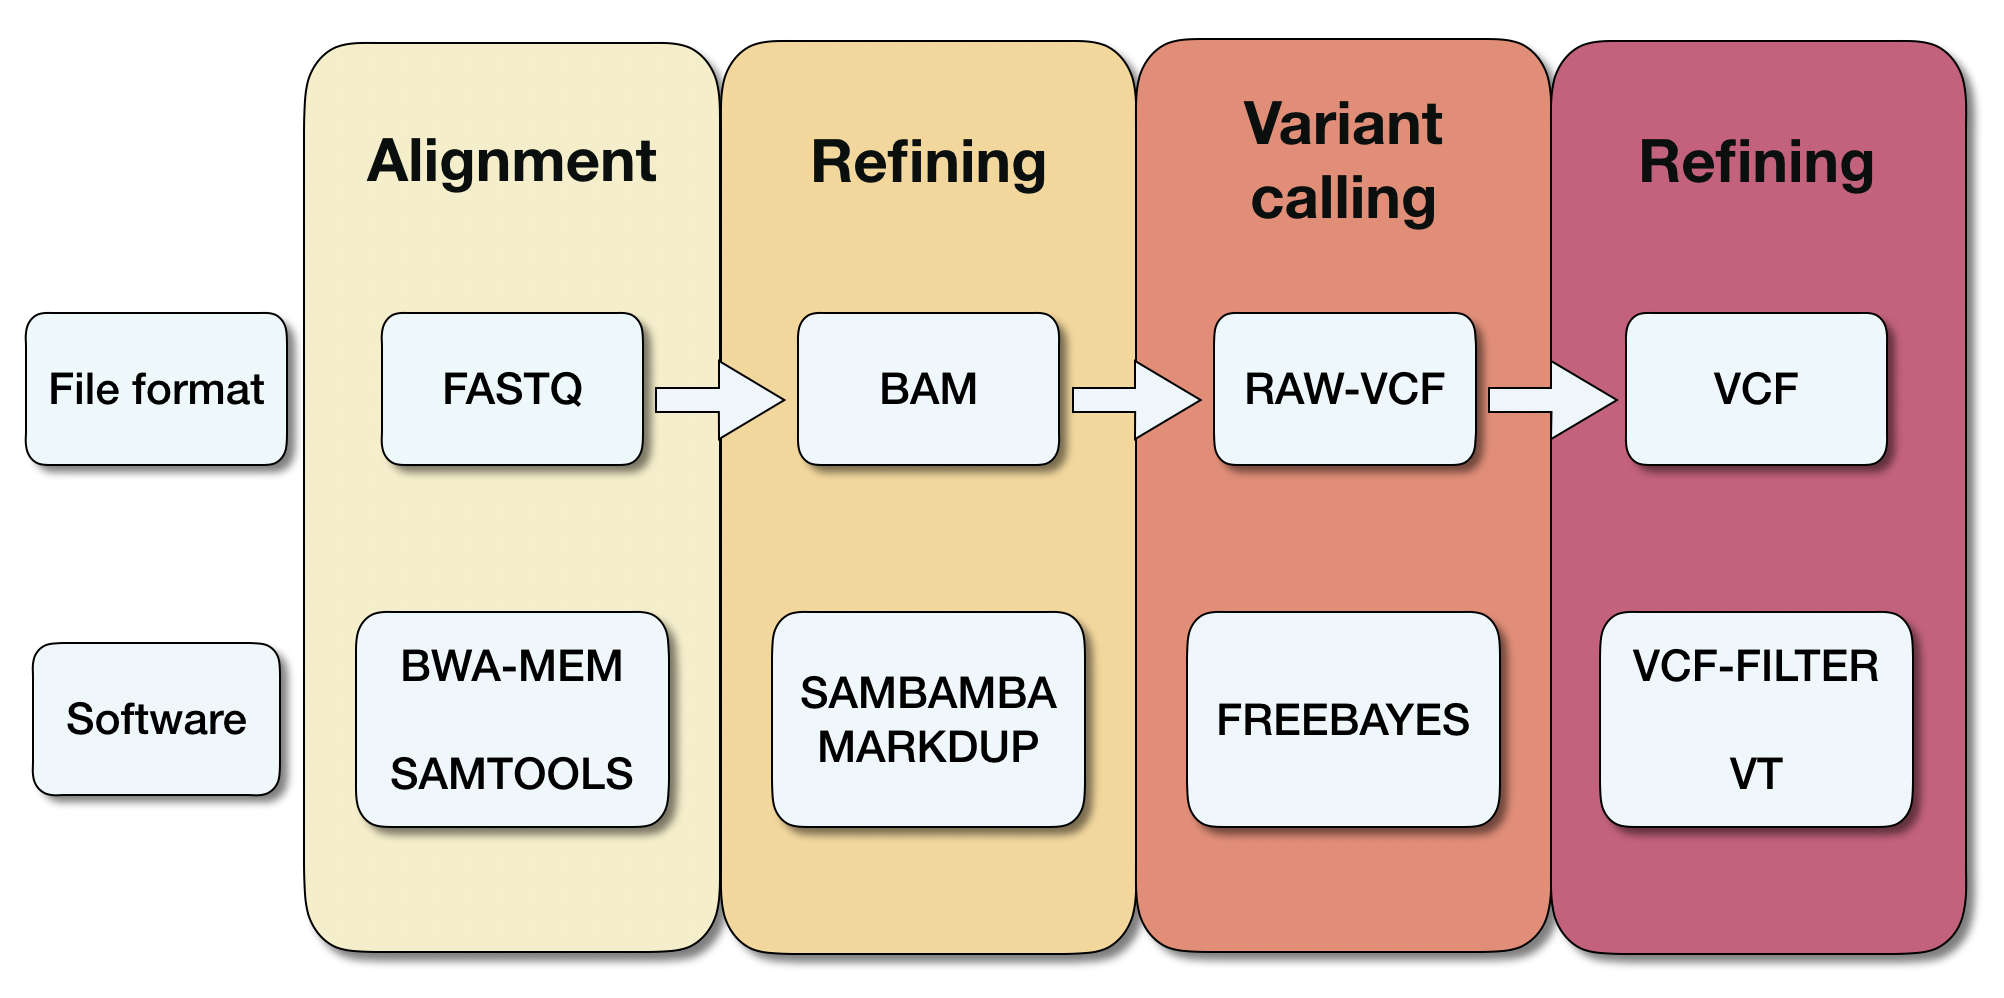
\includegraphics[width=0.7\textwidth]{fig/align-ref-vc.png}
\decoRule
\caption{\textbf{Pipeline for identification of genetic variants.} Sequencing reads are stored in fastq files. The first step is the \textit{alignment} of the reads against the reference genome that produces a bam file. Aligned reads are \textit{refined} and used for \textit{variant calling} that produces vcf files.}
\label{fig:align-ref-vc}
\end{figure}

\vspace{0.5cm}

I performed the \textbf{alignment} of the raw sequence data in form of \gls{reads} against the human reference Genome (GRChg38.p12, \cite{rosenbloom2015ucsc}) using \textsc{bwa-mem} \cite{li2013aligning} and \textsc{samtools} \cite{li2009sequence}. The alignment produces files in the \gls{bam} format that provide information on the quality of the alignemnt and enable some quality controls. In our data set the majority of the reads were correctly aligned to the reference genome.  \newline
Before proceeding to the next step I used \textsc{sambamba} \cite{tarasov2015sambamba} to \textbf{refine} the data and remove PCR duplicates, i.e. reads and they came from the same DNA fragment that bias variant detection through increased homozygosity.\newline

I used the refined bam file to perform \textbf{variant calling} using \textsc{freebayes} \cite{garrison2012haplotype} that produces data in the \gls{vcf} format. The variant calling is the process of identification of variants from sequence data, where variants are chunks of sequence that differ from the reference genome. Genetic variants are classified as single nucleotide variants (SNVs), small insertions and deletions (indels), and structural variants (SVs, large genomic rearrangements). In addition, to call variants, the software specifies whether samples are homozygous or heterozygous (genotype) at the variable sites and the \gls{genotype likelihood}, i.e. the probability that the observed genotype is correct. \newline

The final step is a second round of \textbf{refining} that includes three steps. 
\begin{itemize}
    \item I used \textsc{vcffilter} \cite{vcflib} to filter variants for \gls{quality score}(QUAL)>20. The QUAL is an estimate of how likely it is to observe a call by chance, and a value of 20 corresponds to 1\% probability of having an incorrect genotype.\\
    \item I used \textsc{vt} \cite{tan2015unified} to do the normalization that consist of two parts: parsimony and left alignment. Parsimony is the representation of a variant in as few nucleotides as possible without reducing the length of any allele to 0. Left alignment is the shift of the start position of a variant to the left till it is no longer possible to do so (Figure \ref{fig:vtNorm} \cite{tan2015unified}).\\



    \item I used \textsc{vt} to deconstruct multiallelic variants in a VCF to allow for allelic comparisons between call sets (Figure \ref{fig:vtDecomp}) \cite{tan2015unified}.\\
\end{itemize}

Overall, the variant calling identified on average 4.7M variant site \textit{per} sample. This number corresponds to the expectation in individuals of European ancestry \cite{1000genome2015global}. The most represented class is single nucleotide variant (83.2\%) followed by insertions (6.85\% ) and deletions (6.84\%)(Figure \ref{fig:variantClass}, \ref{fig:percentVariantClass})

\begin{figure}[H]
\centering
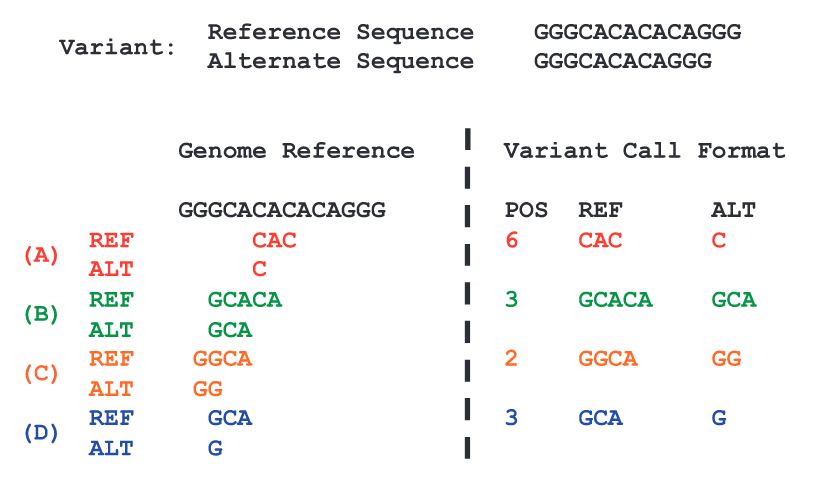
\includegraphics[width=0.55\textwidth]{fig/vtNormalizeTan.png}
\decoRule
\caption{\textbf{Normalization.} Example  of  VCF  entries  representing  the  same  variant. Left  panel aligns each allele to the reference genome, and the right panel represents the variant in VCF. (A) is not left-aligned (B) is neither left-aligned nor parsimonious, (C) is not parsimonious and (D) is normalized. \textit{ Adapted from \cite{tan2015unified}}}
\label{fig:vtNorm}
\end{figure}

\vspace{2cm}

\begin{figure}[H]
\centering
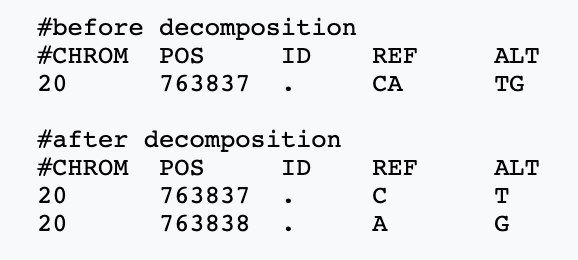
\includegraphics[width=0.55\textwidth]{fig/vtDecompose.png}
\decoRule
\caption{\textbf{Decompositon} Biallelic clumped variant are decomposed for allelic comparisons between call sets} \textit{ Adapted from \cite{tan2015unified}}. 
\label{fig:vtDecomp}
\end{figure}

\begin{figure}[H]
\centering
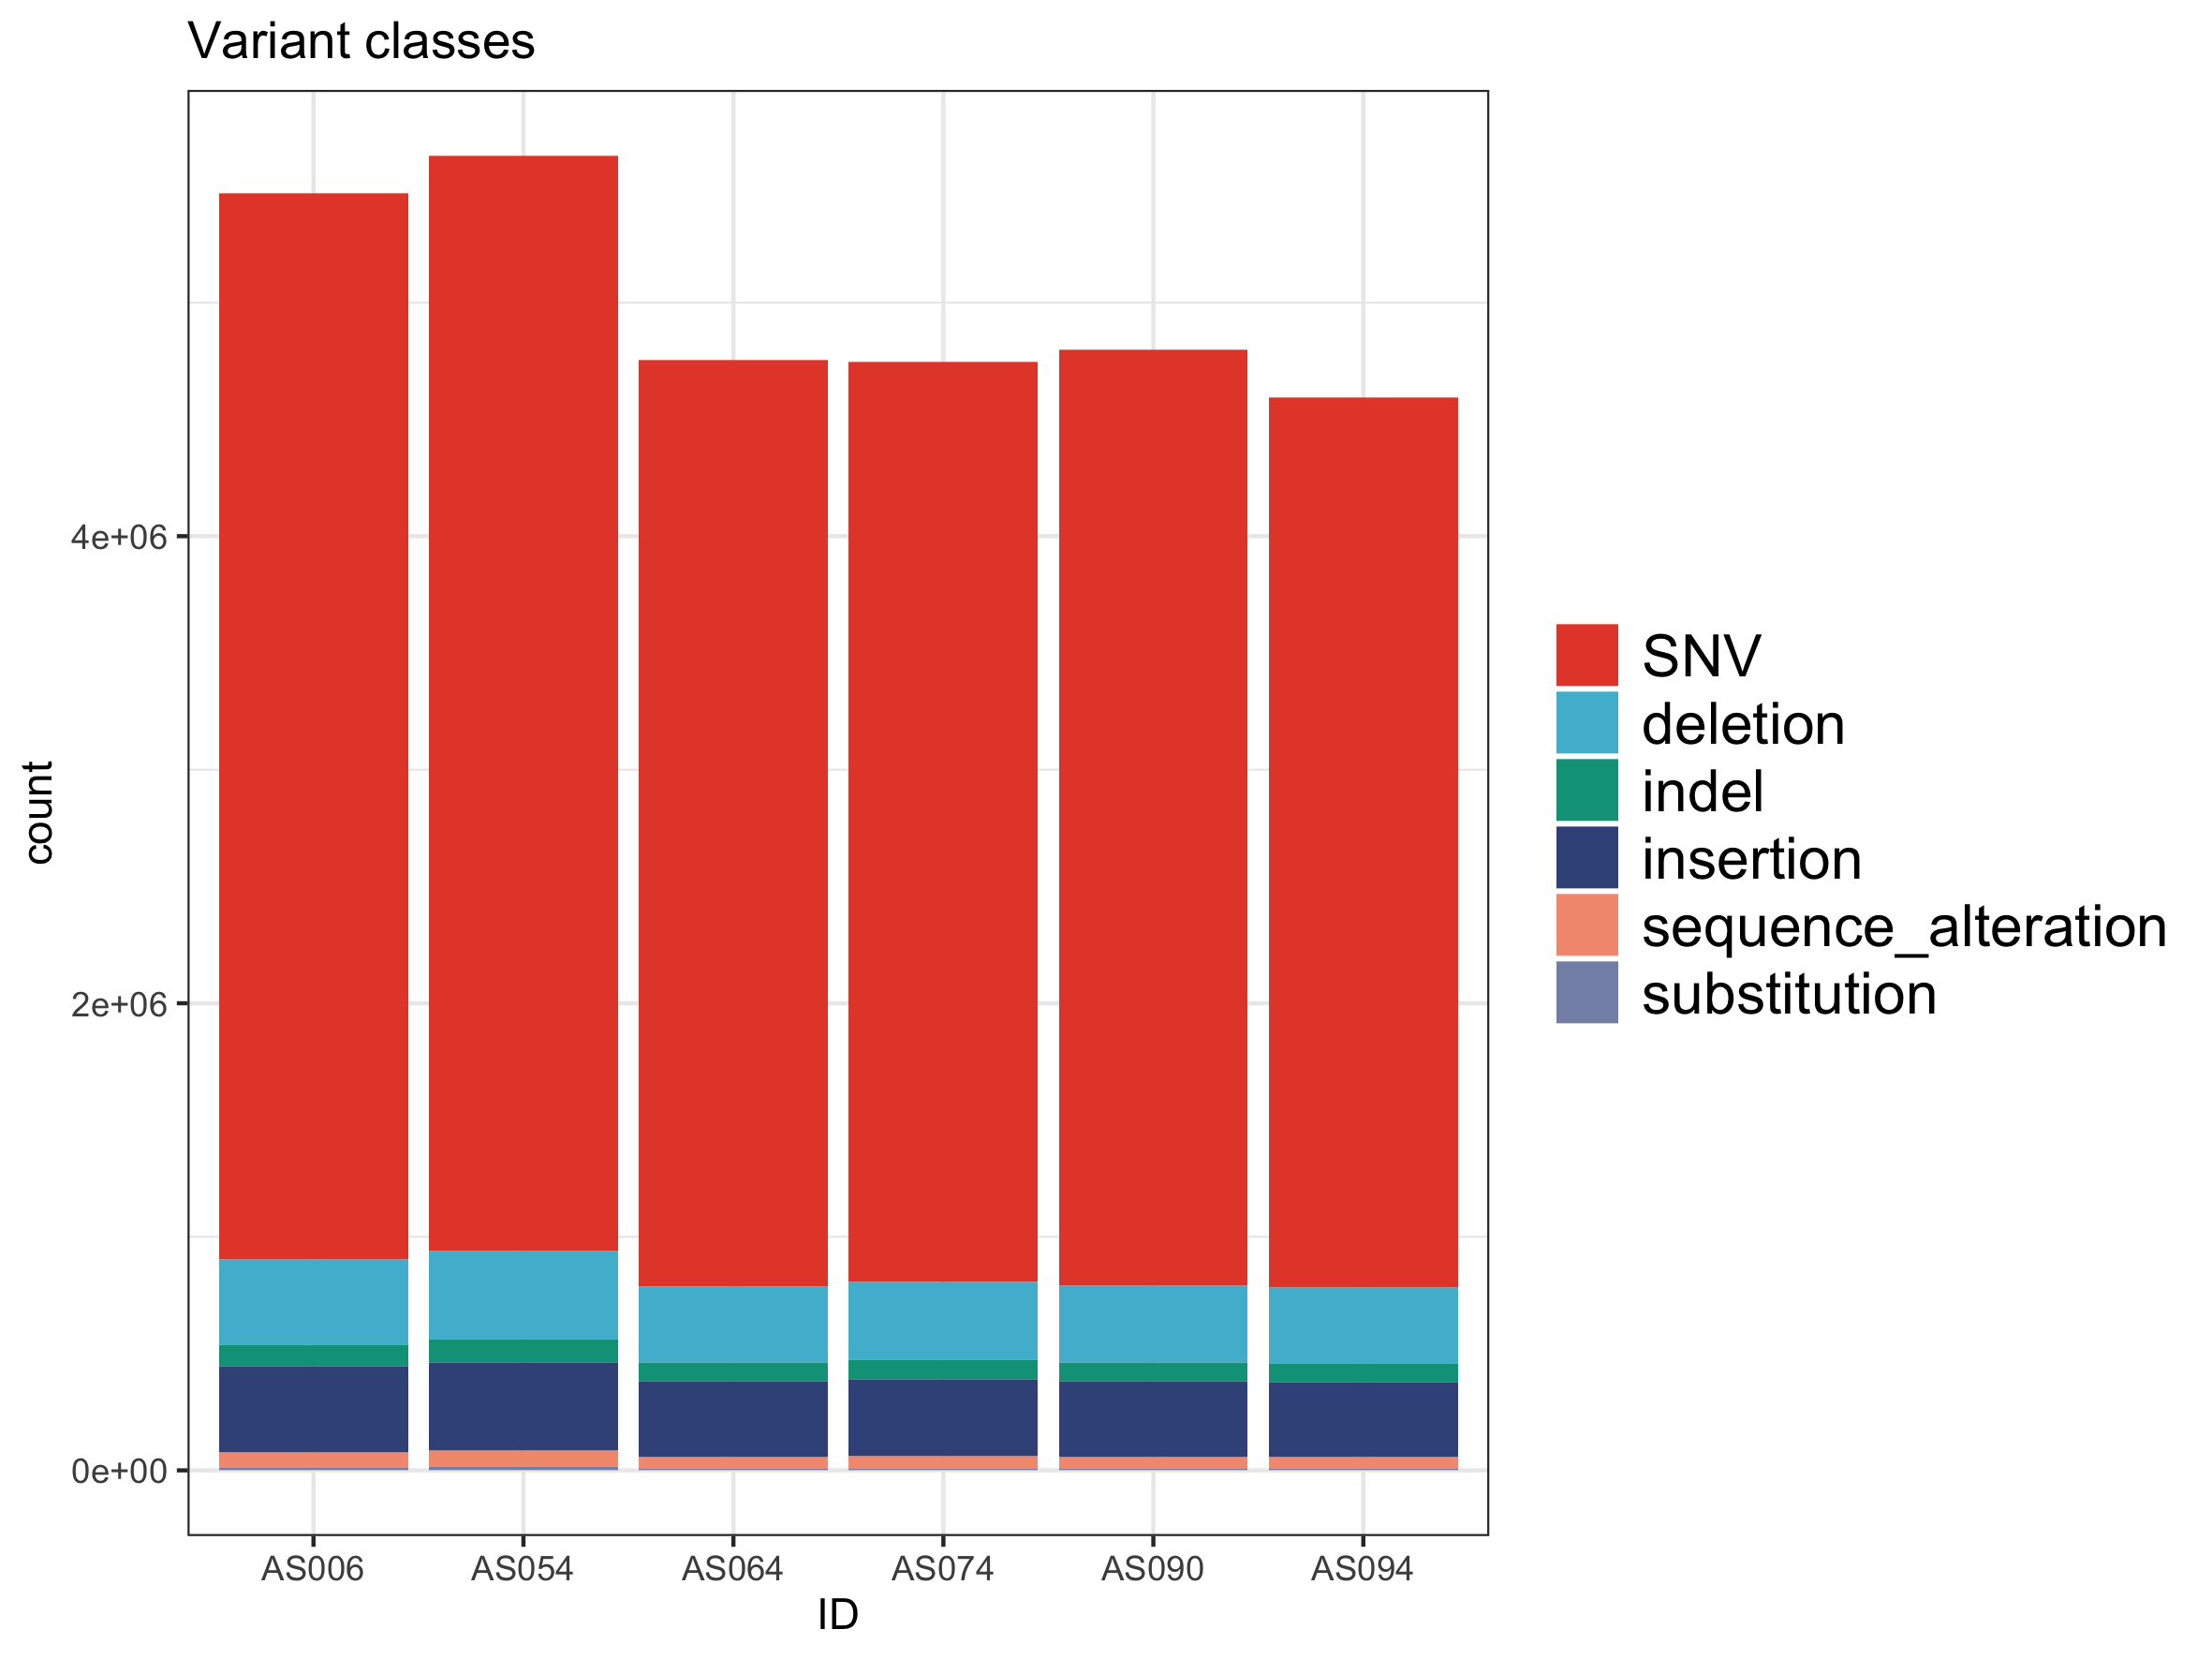
\includegraphics[width=0.55\textwidth]{fig/variantClass.png}
\decoRule
\caption{\textbf{Counts of variants types per sample.} The most represented class is single nucleotide variant (83.2\%) followed by insertions (6.85\% ) and deletions (6.84\% }
\label{fig:variantClass}
\end{figure}

\vspace{1.5cm}

\begin{figure}[H]
\centering
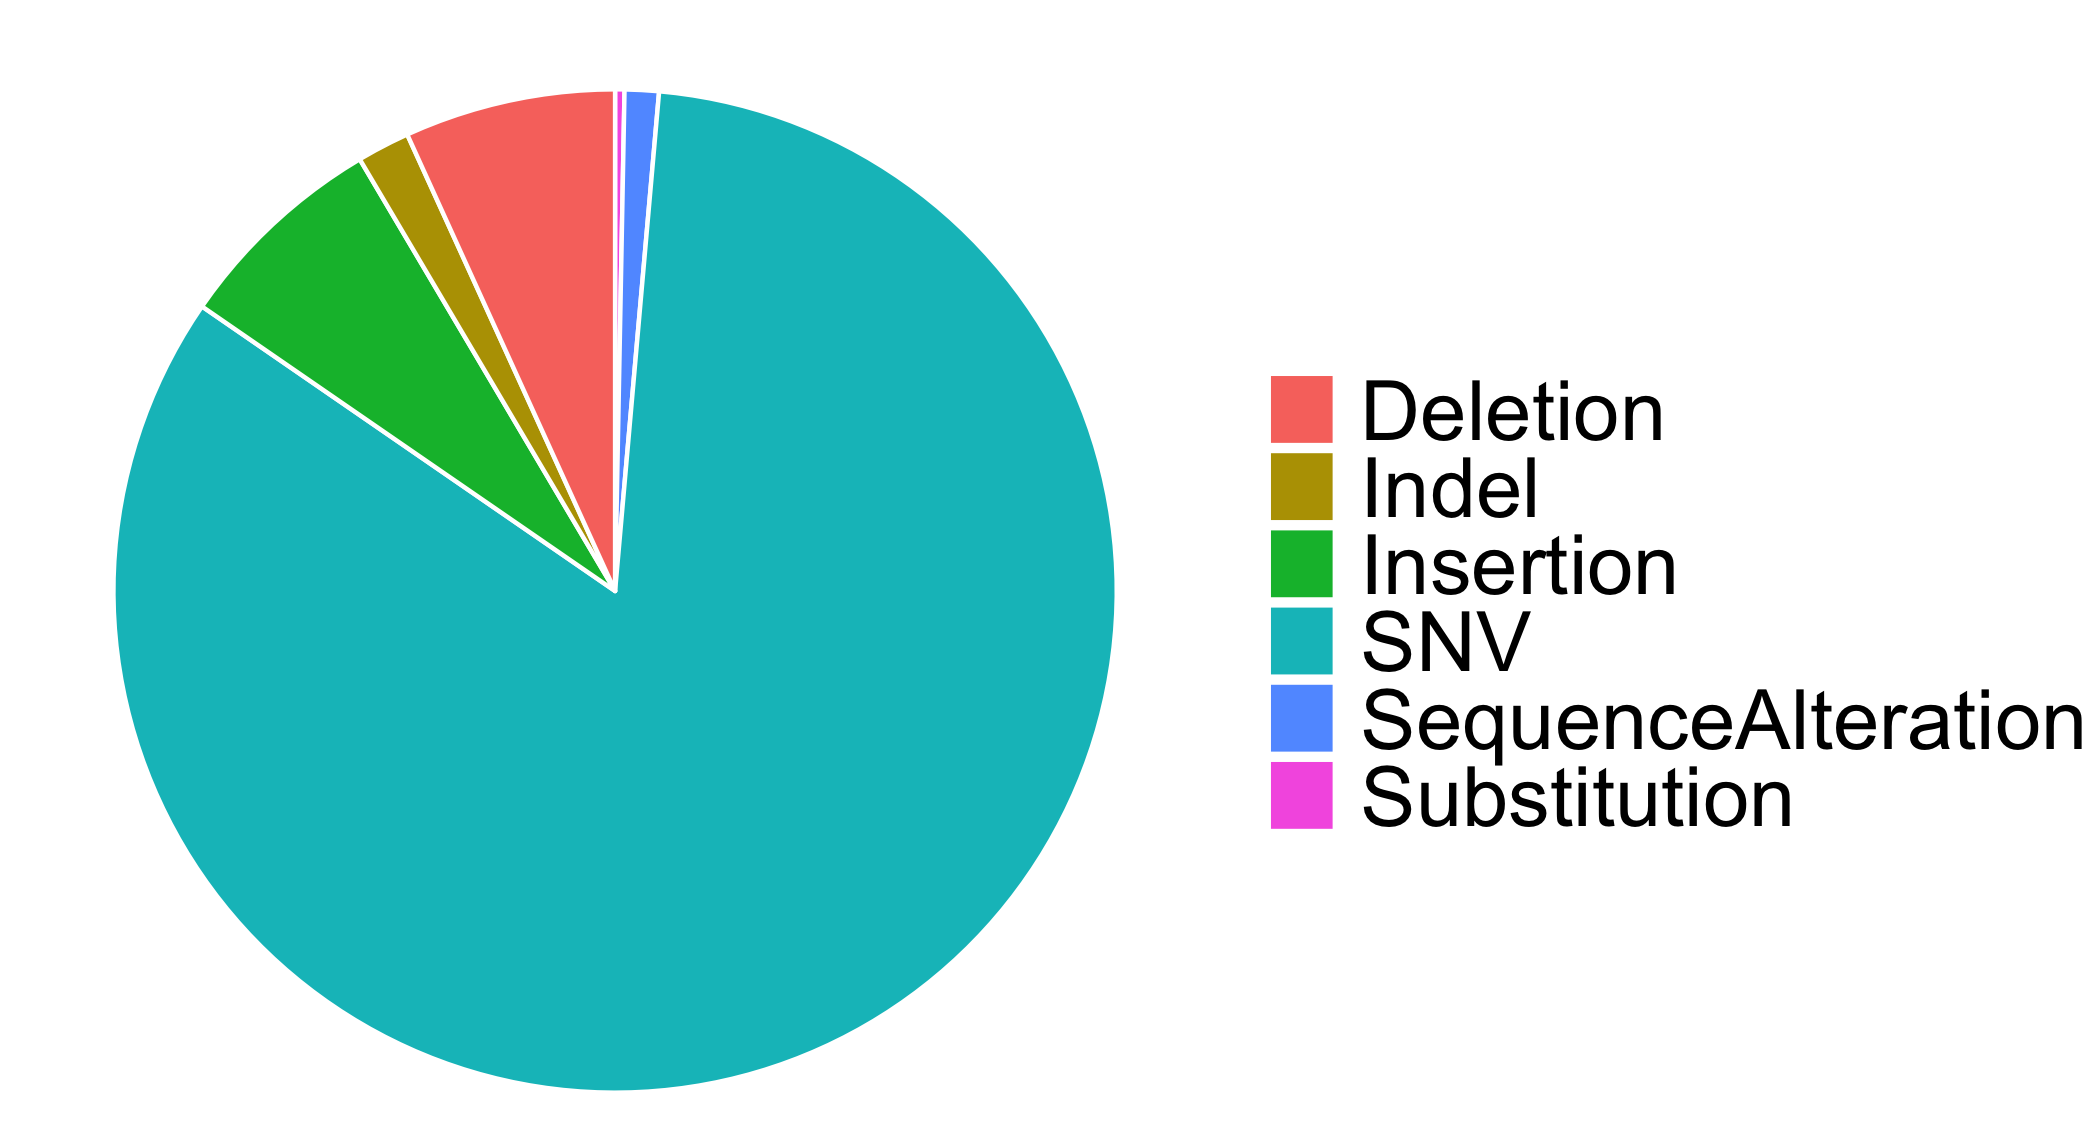
\includegraphics[width=0.55\textwidth]{fig/PieVariantClass.png}
\decoRule
\caption{\textbf{Average prevalence of variant types among samples}. SNV 83.2\%, insertion 6.85\%, deletion 6.84\%, indel 1.7\%, sequence alteration 1.05\%, substitution 0.2\%}
\label{fig:percentVariantClass}
\end{figure}


%%%%%%%%%%%%%%%%%%%%%%%%%%%%%%%%%%%%%%%%%%%%%%%%%%%%%%%%%%%%%%%%%%%%%%%%%%%%%%%%%%%%%%%
%  Subsection 
%%%%%%%%%%%%%%%%%%%%%%%%%%%%%%%%%%%%%%%%%%%%%%%%%%%%%%%%%%%%%%%%%%%%%%%%%%%%%%%%%%%%%%%

\subsection{Functional annotation of genetic variants}

Once the genetic variants are identified, the following challenge is to understand their functional consequences, i.e.the effect that they produce on the gene and if they cause a specific phenotype. I have used \textsc{variant effect predictor} \textsc{vep}, \cite{mclaren2016ensembl} provided by Ensembl \cite{howe2020ensembl} to annotate the genetic variant discovered in the six GREP samples. \textsc{vep} is currently the most updated and comprehensive toolset for the analysis, annotation, and prioritization of genomic variants in the coding and non-coding regions based on an extensive collection of genomic annotations. \textsc{vep} can determine the effect of variants (SNPs, insertions, deletions, CNVs or structural variants) on genes, transcripts, and protein sequence, as well as regulatory regions.\newline

{\small
\begin{sidewaystable}
\caption{Table of Consequences}
\label{tab:csqVEP}
\centering
\begin{adjustbox}{width=1\textwidth}
\begin{tabular}{c c c c}
\toprule
\tabhead{SO term} & \tabhead{SO description} & \tabhead{SO accession} & \tabhead{Impact} \\
\midrule
transcript ablation & A feature ablation whereby the deleted region includes a transcript feature & SO:0001893 & HIGH \\
splice acceptor variant & A splice variant that changes the 2 base region at the 3' end of an intron & SO:0001574 & HIGH \\
splice donor variant & A splice variant that changes the 2 base region at the 5' end of an intron & SO:0001575 & HIGH \\
stop gained & A sequence variant whereby at least one base of a codon is changed, resulting in a premature stop codon, leading to a shortened transcript & SO:0001587 & HIGH \\
frameshift variant & A sequence variant which causes a disruption of the translational reading frame, because the number of nucleotides inserted or deleted is not a multiple of three & SO:0001589 & HIGH \\
stop lost & A sequence variant where at least one base of the terminator codon (stop) is changed, resulting in an elongated transcript & SO:0001578 & HIGH \\
start lost & A codon variant that changes at least one base of the canonical start codon & SO:0002012 & HIGH \\
transcript amplification & A feature amplification of a region containing a transcript & SO:0001889 & HIGH \\
inframe insertion & An inframe non synonymous variant that inserts bases into in the coding sequence & SO:0001821 & MODERATE \\
inframe deletion & An inframe non synonymous variant that deletes bases from the coding sequence & SO:0001822 & MODERATE \\
missense variant & A sequence variant, that changes one or more bases, resulting in a different amino acid sequence but where the length is preserved & SO:0001583 & MODERATE \\
protein altering variant & A sequence variant which is predicted to change the protein encoded in the coding sequence & SO:0001818 & MODERATE \\
splice region variant & A sequence variant in which a change has occurred within the region of the splice site, either within 1-3 bases of the exon or 3-8 bases of the intron & SO:0001630 & LOW \\
incomplete terminal codon variant & A sequence variant where at least one base of the final codon of an incompletely annotated transcript is changed & SO:0001626 & LOW \\
start retained variant & A sequence variant where at least one base in the start codon is changed, but the start remains & SO:0002019 & LOW \\
stop retained variant & A sequence variant where at least one base in the terminator codon is changed, but the terminator remains & SO:0001567 & LOW \\
synonymous variant & A sequence variant where there is no resulting change to the encoded amino acid & SO:0001819 & LOW \\
coding sequence variant & A sequence variant that changes the coding sequence & SO:0001580 & MODIFIER \\
mature miRNA variant & A transcript variant located with the sequence of the mature miRNA & SO:0001620 & MODIFIER \\
5 prime UTR variant & A UTR variant of the 5' UTR & SO:0001623 & MODIFIER \\
3 prime UTR variant & A UTR variant of the 3' UTR & SO:0001624 & MODIFIER \\
non coding transcript exon variant & A sequence variant that changes non-coding exon sequence in a non-coding transcript & SO:0001792 & MODIFIER \\
intron variant & A transcript variant occurring within an intron & SO:0001627 & MODIFIER \\
NMD transcript variant & A variant in a transcript that is the target of NMD & SO:0001621 & MODIFIER \\
non coding transcript variant & A transcript variant of a non coding RNA gene & SO:0001619 & MODIFIER \\
upstream gene variant & A sequence variant located 5' of a gene & SO:0001631 & MODIFIER \\
downstream gene variant & A sequence variant located 3' of a gene & SO:0001632 & MODIFIER \\
TFBS ablation & A feature ablation whereby the deleted region includes a transcription factor binding site & SO:0001895 & MODIFIER \\
TFBS amplification & A feature amplification of a region containing a transcription factor binding site & SO:0001892 & MODIFIER \\
TF binding site variant & A sequence variant located within a transcription factor binding site & SO:0001782 & MODIFIER \\
regulatory region ablation & A feature ablation whereby the deleted region includes a regulatory region & SO:0001894 & MODERATE \\
regulatory region amplification & A feature amplification of a region containing a regulatory region & SO:0001891 & MODIFIER \\
feature elongation & A sequence variant that causes the extension of a genomic feature, with regard to the reference sequence & SO:0001907 & MODIFIER \\
regulatory region variant & A sequence variant located within a regulatory region & SO:0001566 & MODIFIER \\
feature truncation & A sequence variant that causes the reduction of a genomic feature, with regard to the reference sequence & SO:0001906 & MODIFIER \\
intergenic variant & A sequence variant located in the intergenic region, between genes & SO:0001628 & MODIFIER \\
\bottomrule\\
\end{tabular}
\end{adjustbox}
\end{sidewaystable}
}

Table \ref{tab:csqVEP} (adapted from \cite{mclaren2016ensembl}) describes the classification of the consequences in the Ensembl Variation database. The impact of the variant on the gene product is classified into four categories: high, moderate, low, and modifier. Examples of variations with high impact are mutations that cause premature termination of the transcription (stop gained) or that suppress transcription (start lost). The classification includes variants in genic (e.g. missense), regulatory (e.g. located in transcription factor binding site) and intergenic regions. In the analysis of the GREP samples, we refer to these categories. 



Figure \ref{fig:grid_cons} shows the outcome of \textsc{vep} stratified by categories of impact. All sample present very similar patterns as shown in Table \ref{tab:percentageImpact} showing percentage for each category of impact. Among the variants with high impact the most represented is Splice donor variant, followed by Splice acceptor and frameshift variants (Figure \ref{fig:grid_cons}.A). Almost all variants with moderate impact are missense variants (99\%, Figure \ref{fig:grid_cons}.B). Among variants with low impact, there is a prevalence of synonymous (68.5\%) and splice region (31.3\%) variants. Finally, the more common variants among modifiers are intron (50.6\%) and intergenic (34.8\%) variants. 

\vspace{1cm}

\begin{figure}[H]
\centering
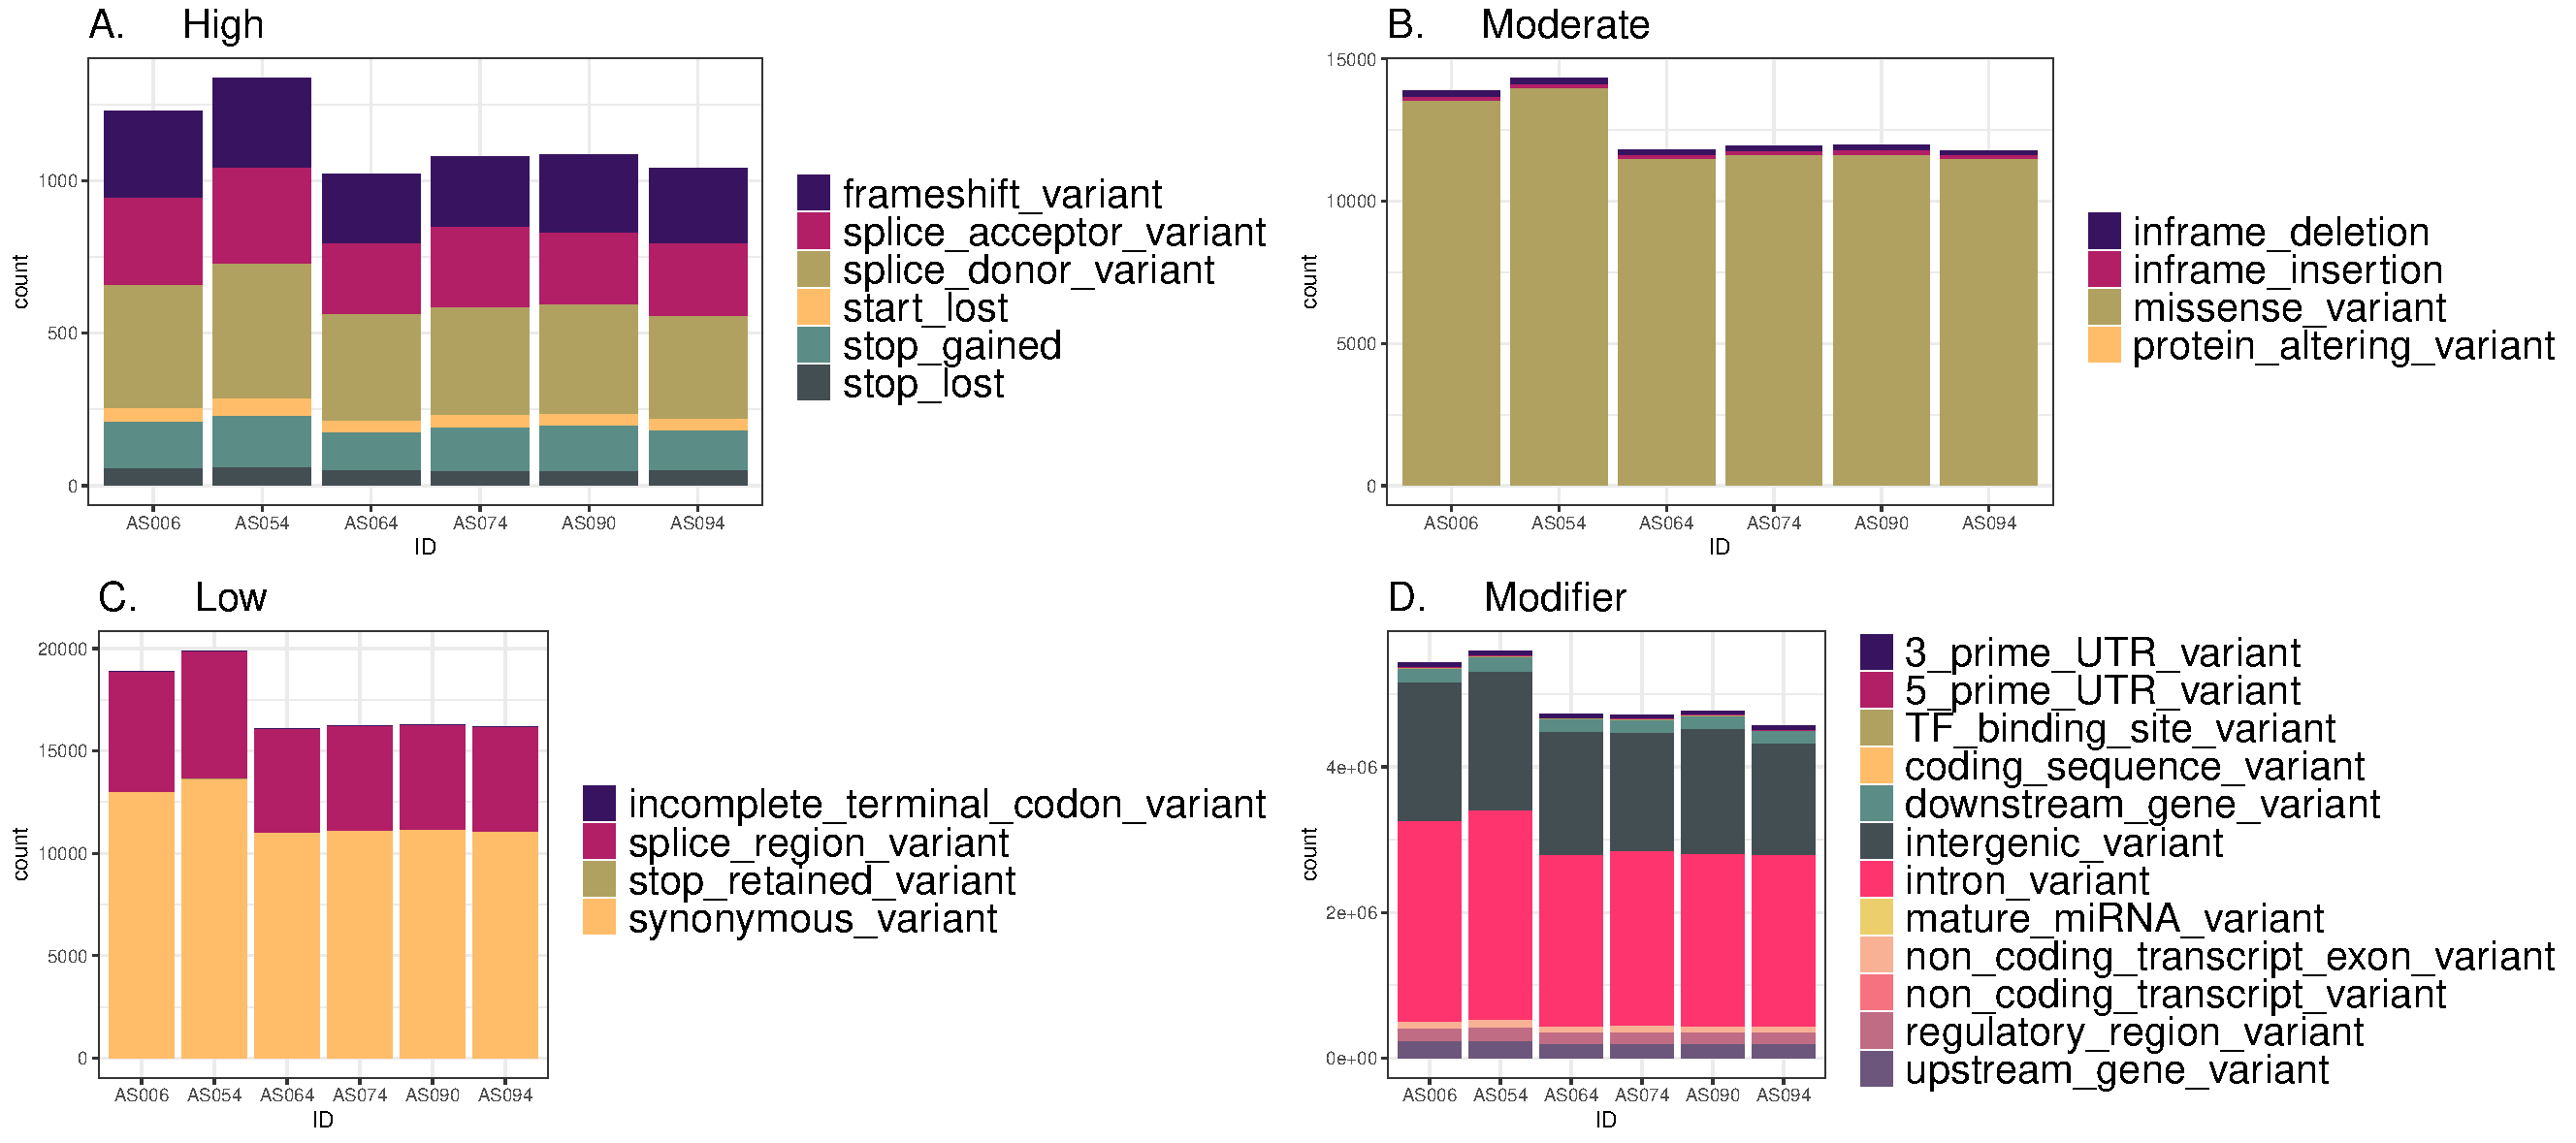
\includegraphics[width=1\textwidth]{fig/grid_cons.pdf}
\decoRule
\caption{\textbf{Functional classification of genetic variants stratified by the impact of the variant.} \textbf{Fig A High:} The most represented category is Splice donor variant, followed by Splice acceptor and frameshift variants. \textbf{Fig B Moderate:} Almost all variants with moderate impact are missense variants. \textbf{Fig C Low:} Prevalence of synonymous and splice region variants.\textbf{Fig D Modifier:} The most common categories are intron and inter-genic}
\label{fig:grid_cons}
\end{figure}


{\small
\begin{table}
\caption{Fraction variants in class of impact}
\label{tab:percentageImpact}
\centering
\begin{adjustbox}{width=0.7\textwidth}
\begin{tabular}{1 1 1 1 1 }
\toprule
\tabhead{Sample} & \tabhead{HIGH} & \tabhead{MODERATE} & \tabhead{LOW} & \tabhead{MODIFIER} \\
\midrule
 AS006 & 0.022 & 0.254 & 0.345 & 99.4 \\
 AS054 & 0.023 & 0.254 & 0.353 & 99.4 \\
 AS064 & 0.021 & 0.249 & 0.339 & 99.4 \\
 AS074 & 0.022 & 0.252 & 0.342 & 99.4 \\
 AS090 & 0.022 & 0.249 & 0.340 & 99.4 \\
 AS094 & 0.022 & 0.257 & 0.352 & 99.4 \\
\bottomrule\\
\end{tabular}
\end{adjustbox}
\end{table}
}

%%%%%%%%%%%%%%%%%%%%%%%%%%%%%%%%%%%%%%%%%%%%%%%%%%%%%%%%%%%%%%%%%%%%%%%%%%%%%%%%%%%%%%%%%%%%
%  Subsection 
%%%%%%%%%%%%%%%%%%%%%%%%%%%%%%%%%%%%%%%%%%%%%%%%%%%%%%%%%%%%%%%%%%%%%%%%%%%%%%%%%%%%%%%%%%%%
\subsection{Development of a pipeline for variant prioritization}
The rationale behind the identification of genetic variants responsible for PL is based on the hypotheses that the causative variants are likely to be among those classified as detrimental and that more than one mutation can contribute to the phenotype. Furthermore, we assume that the phenotype is a complex trait, i.e. the combination of variants at more than one gene might have caused the miscarriage, therefore we seek a list of variants in more than one gene or regulatory region, rather than a single variant. Under these assumptions, I used the information contained in the variant annotations to search for those more likely to be deleterious and possibly causative.\\

I contributed to develop a pipeline (\url{https://github.com/ezcn/grep}) that analyzes \textbf{genomic variants} within individual genome sequences to prioritize those possibly causative. A scheme of how the algorithm work is presented in Figure \ref{fig:scriptPipeline}. The pipeline is optimized for genomic regions containing coding sequences, while the analysis of regulatory regions is under development. In particular, in this first version of the pipeline we use a combination of the following information: 

%%%%%%%
\begin{figure}[H]
\centering
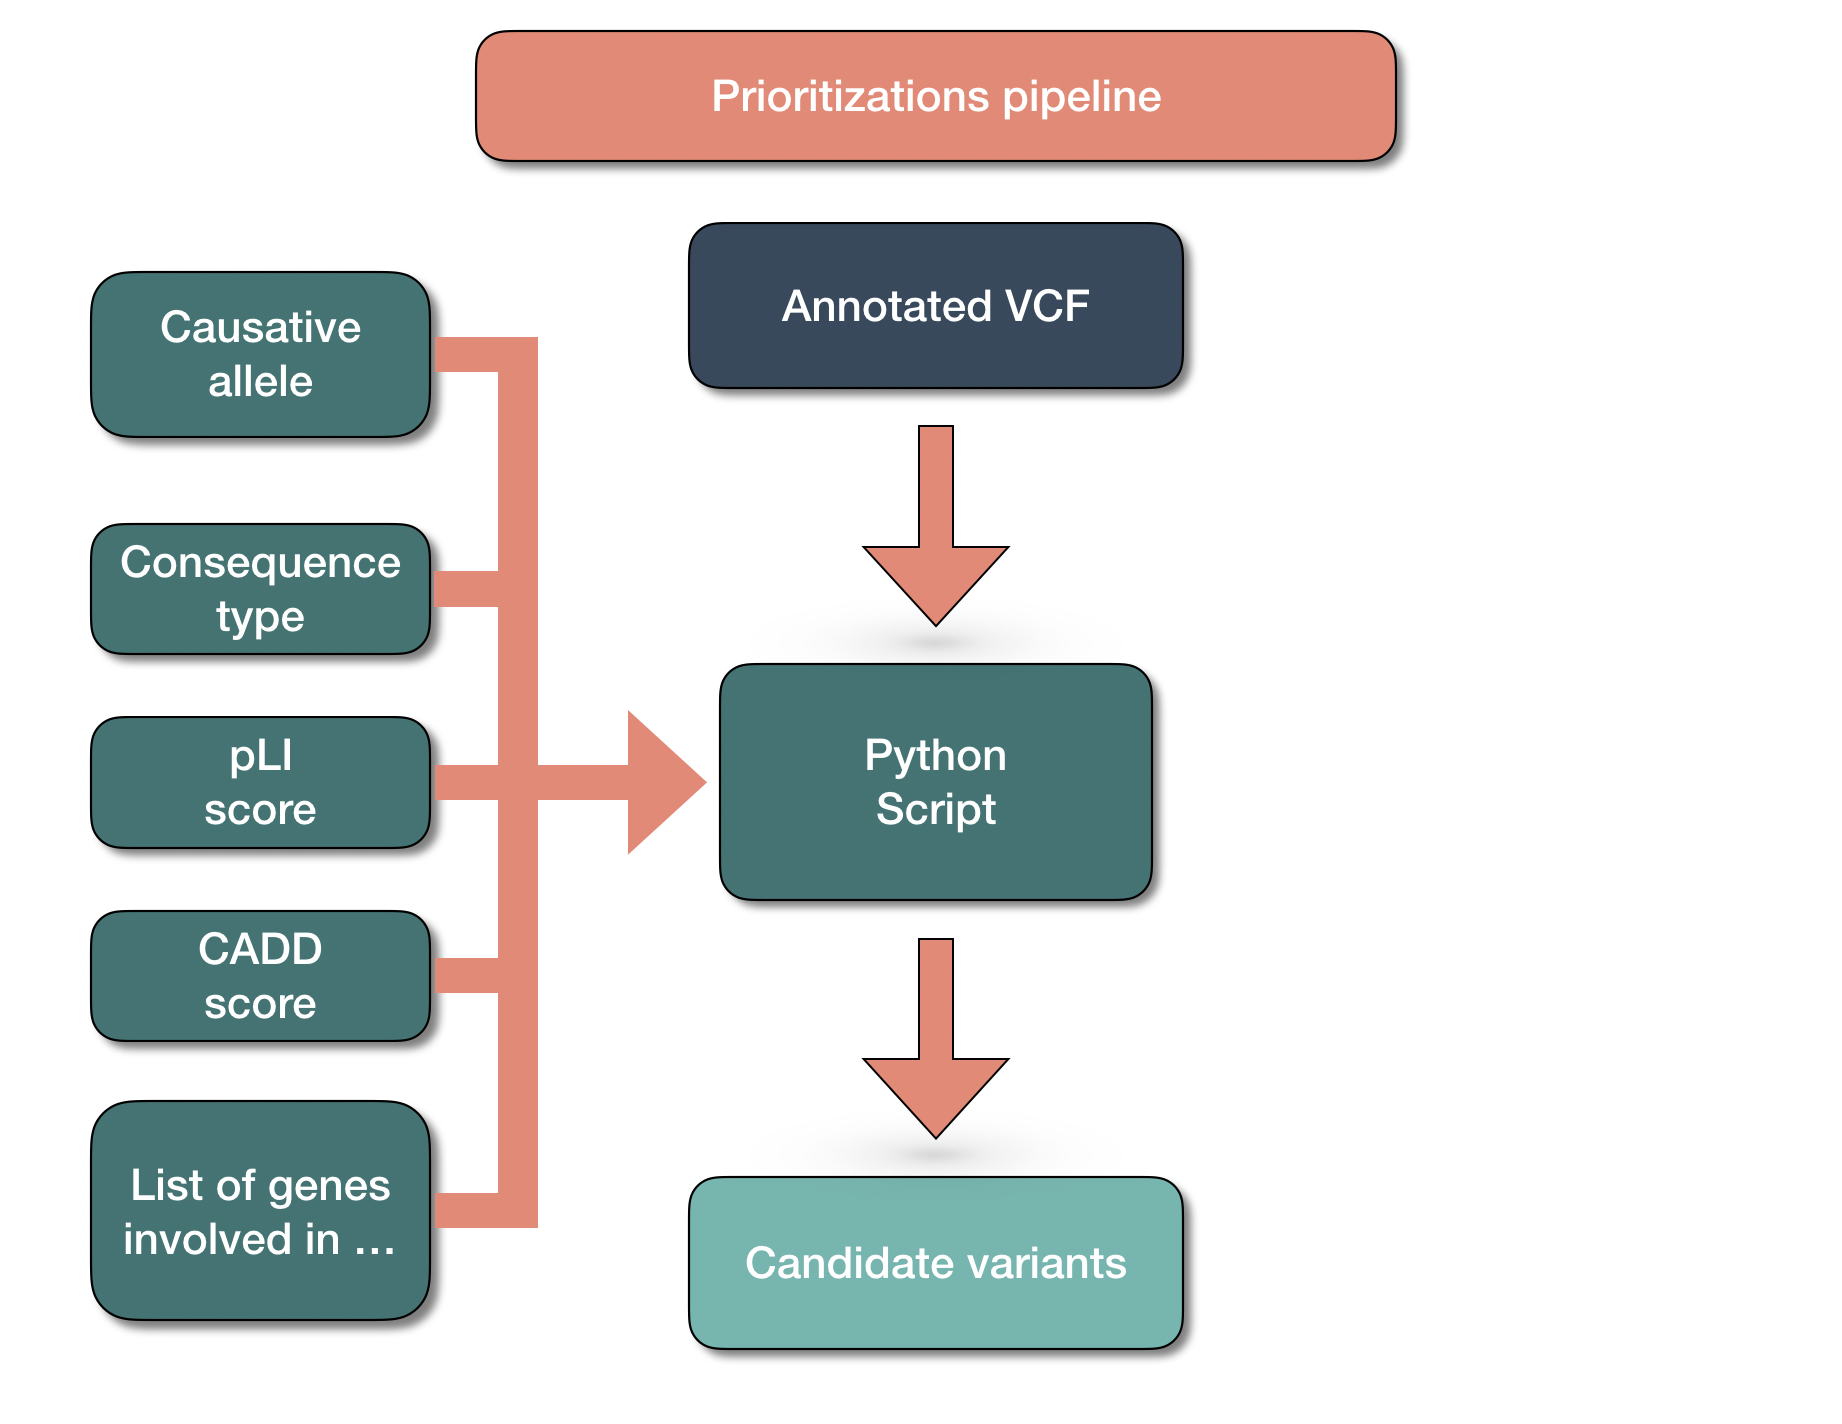
\includegraphics[width=0.85\textwidth]{fig/scriptPipeline.png}
\decoRule
\caption{\textbf{Pipeline for variant prioritization.} The pipeline combines information from variants (functional scores) and from genes to filter variants likely to be detrimental.}
\label{fig:scriptPipeline}
\end{figure}

\begin{itemize}
\item \textbf{Allele that causes the consequence.} We consider the \textbf{count} of the allele, i.e. if the individual has one or two alleles, assuming that having two alleles is worst than having only one. We consider \textbf{allele frequency} in the 1000Genomes \cite{1000genome2015global} and gnomeAD \cite{karczewskigenome} databases, representing reference population; we assume that if the allele is common than it is less likely to be detrimental. 
\item \textbf{Type and severity of the consequence.} We use the ranking illustrated in Table \ref{tab:csqVEP} to give priorities to consequences with a higher impact on the phenotype. 
\item \textbf{pLI score.} pLI is the probability of a gene of being loss-of-function intolerant \cite{lek2016analysis}. A value of pLI>0.9 suggests that the gene is likely to not tolerate mutations that alter its function, therefore variants located in these genes are more likely to be prioritized. 
\item \textbf{CADD score.} The Combined Annotation Dependent Depletion (CADD) is a score that integrates multiple annotations into one metric by contrasting variants that survived natural selection with simulated mutations \cite{kircher2014general,rentzsch2019cadd}. The highest the CADD score, the more likely is the pathogenicity of a variant and it applies both to coding and non-coding variants. 
\item \textbf{Genes associated with miscarriages or involved in embryonic development.} We assign high priority to variants located in these sets of genes: 4651 essential \cite{blomen2015gene,wang2015identification,hart2015high}; 3801 lethal \cite{dawes2019gene}; genes involved in the embryonic development (GO:0009790); 1853 genes DDD \cite{firth2011deciphering,firth2009decipher}; a manually curated list of genes that have been associated with miscarriages, obtained from literature \cite{laisk2019genetic,pereza2017systematic,qiao2016whole,rull2012genetics,colley2019potential,quintero2017novel}. 
\end{itemize}

The first part of the pipeline works at \textit{per}-individual, \textit{per}-site level producing annotations like those illustrated in Figure \ref{fig:vep_example_output}. Annotations are filtered and ranked in the second part of the pipeline. Overall, the pipeline takes as input the genetic variants in vcf format and produces a table with sites that pass the filtering or have high rank (Figure \ref{fig:scriptPipeline}). 


\begin{figure}[H]
\centering
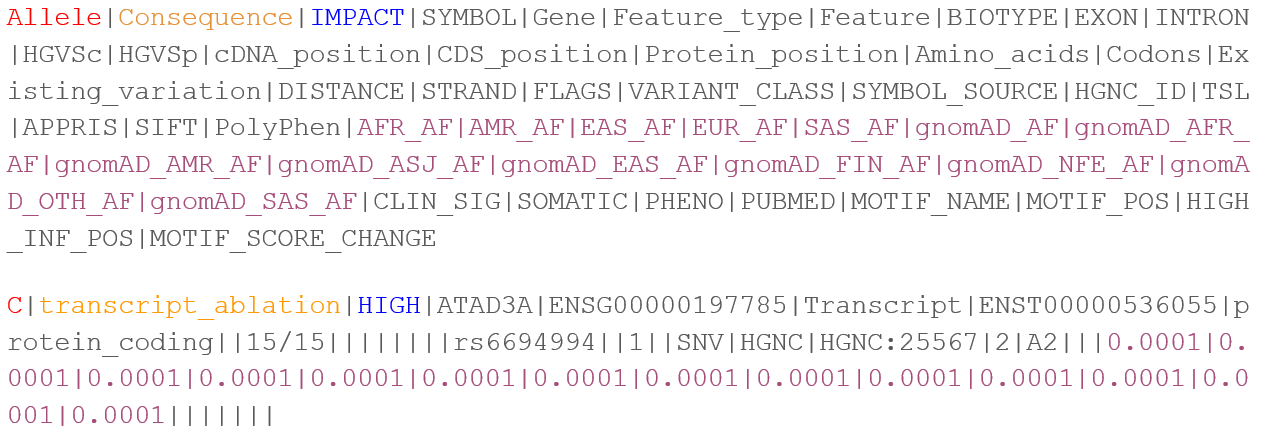
\includegraphics[width=0.9\textwidth]{fig/vep_example_output.PNG}
\decoRule
\caption[Summary Consequence]{\textbf{Header and example output of variant annotation} In the case showed here the C allele has as consequence a transcript ablation, a consequence with high impact on the gene product. This allele has allele frequency 0.0001 in all the populations considered. This is only part of the information considered in the pipeline.}
\label{fig:vep_example_output}
\end{figure}

\subsection{Identification of putatively detrimental variants by filtering and ranking of annotated variants}

\subsubsection{Filtering criteria}
Once variants are annotated, the pipeline filters variants according to different criteria. To target Rare variants with very high CADD score located in genes that are intolerant to loss of function, I used this combination of parameters: 

\begin{itemize}
\item \textbf{Impact.} Only variants with impact HIGH, MODERATE, or LOW. This criterion excludes MODIFIER variants that have a lower impact on the gene's product.
\item \textbf{Threshold for rare variants.} Only variants with frequencies <5\% in the reference populations of the 1000 Genomes and GnomeAD collections. This threshold filters for rare variants but is not too stringent to allow for causative variants to be present in the populations.
\item \textbf{Threshold for pLI score.} Only genes with pLI > 0.9. This value is typical of genes that could not tolerate mutations\cite{lek2016analysis}.
\item \textbf{Threshold for CADD score.} Only variants that have a CADD score above the 90\% percentile. This restricts to variants with highly deleterious consequences. 
\item \textbf{Consequence allele count.} Variants in heterozygosis or homozygosis.
\end{itemize}
\subsubsection{Variants retained after filtering }

When applying the filter described in the paragraph before, we identify 373 unique variants in 112 unique genes. Only one variant has high impact (stop gained), while all other variants are missense substitutions (Table \ref{tab:variatntsAfterCuration}). In each sample we identify one or more variants in 13-27 genes. Figure \ref{fig:filter2output} shows per each sample the CADD and pLI scores for the set of variants retained by the filter (yellow boxes). Notably, there are no variants in homozygosity when using this set of filters. This is expected due to the extreme values of pLI and CADD.\\

\being
{\small
\begin{table}
\caption{Number of genes per individual retained by the filter and after manual curation.}
\label{tab:variatntsAfterCuration}
\centering
\begin{adjustbox}{width=0.6\textwidth}
\begin{tabular}{1 1 1 1}
\toprule
\tabhead{Sample} & \tabhead{Variant consequence} & \tabhead{Number of genes} \\
\midrule
AS006 & missense & 24\\
AS054 & missense & 27\\
AS064 & missense & 25\\
AS074 & missense, stop gained & 23\\
AS090 & missense, stop gained & 13\\
AS094 & missense & 14\\
\bottomrule\\
\end{tabular}
\end{adjustbox}
\end{table}
}

\vspace{1,5cm}

\begin{figure}[H]
\centering
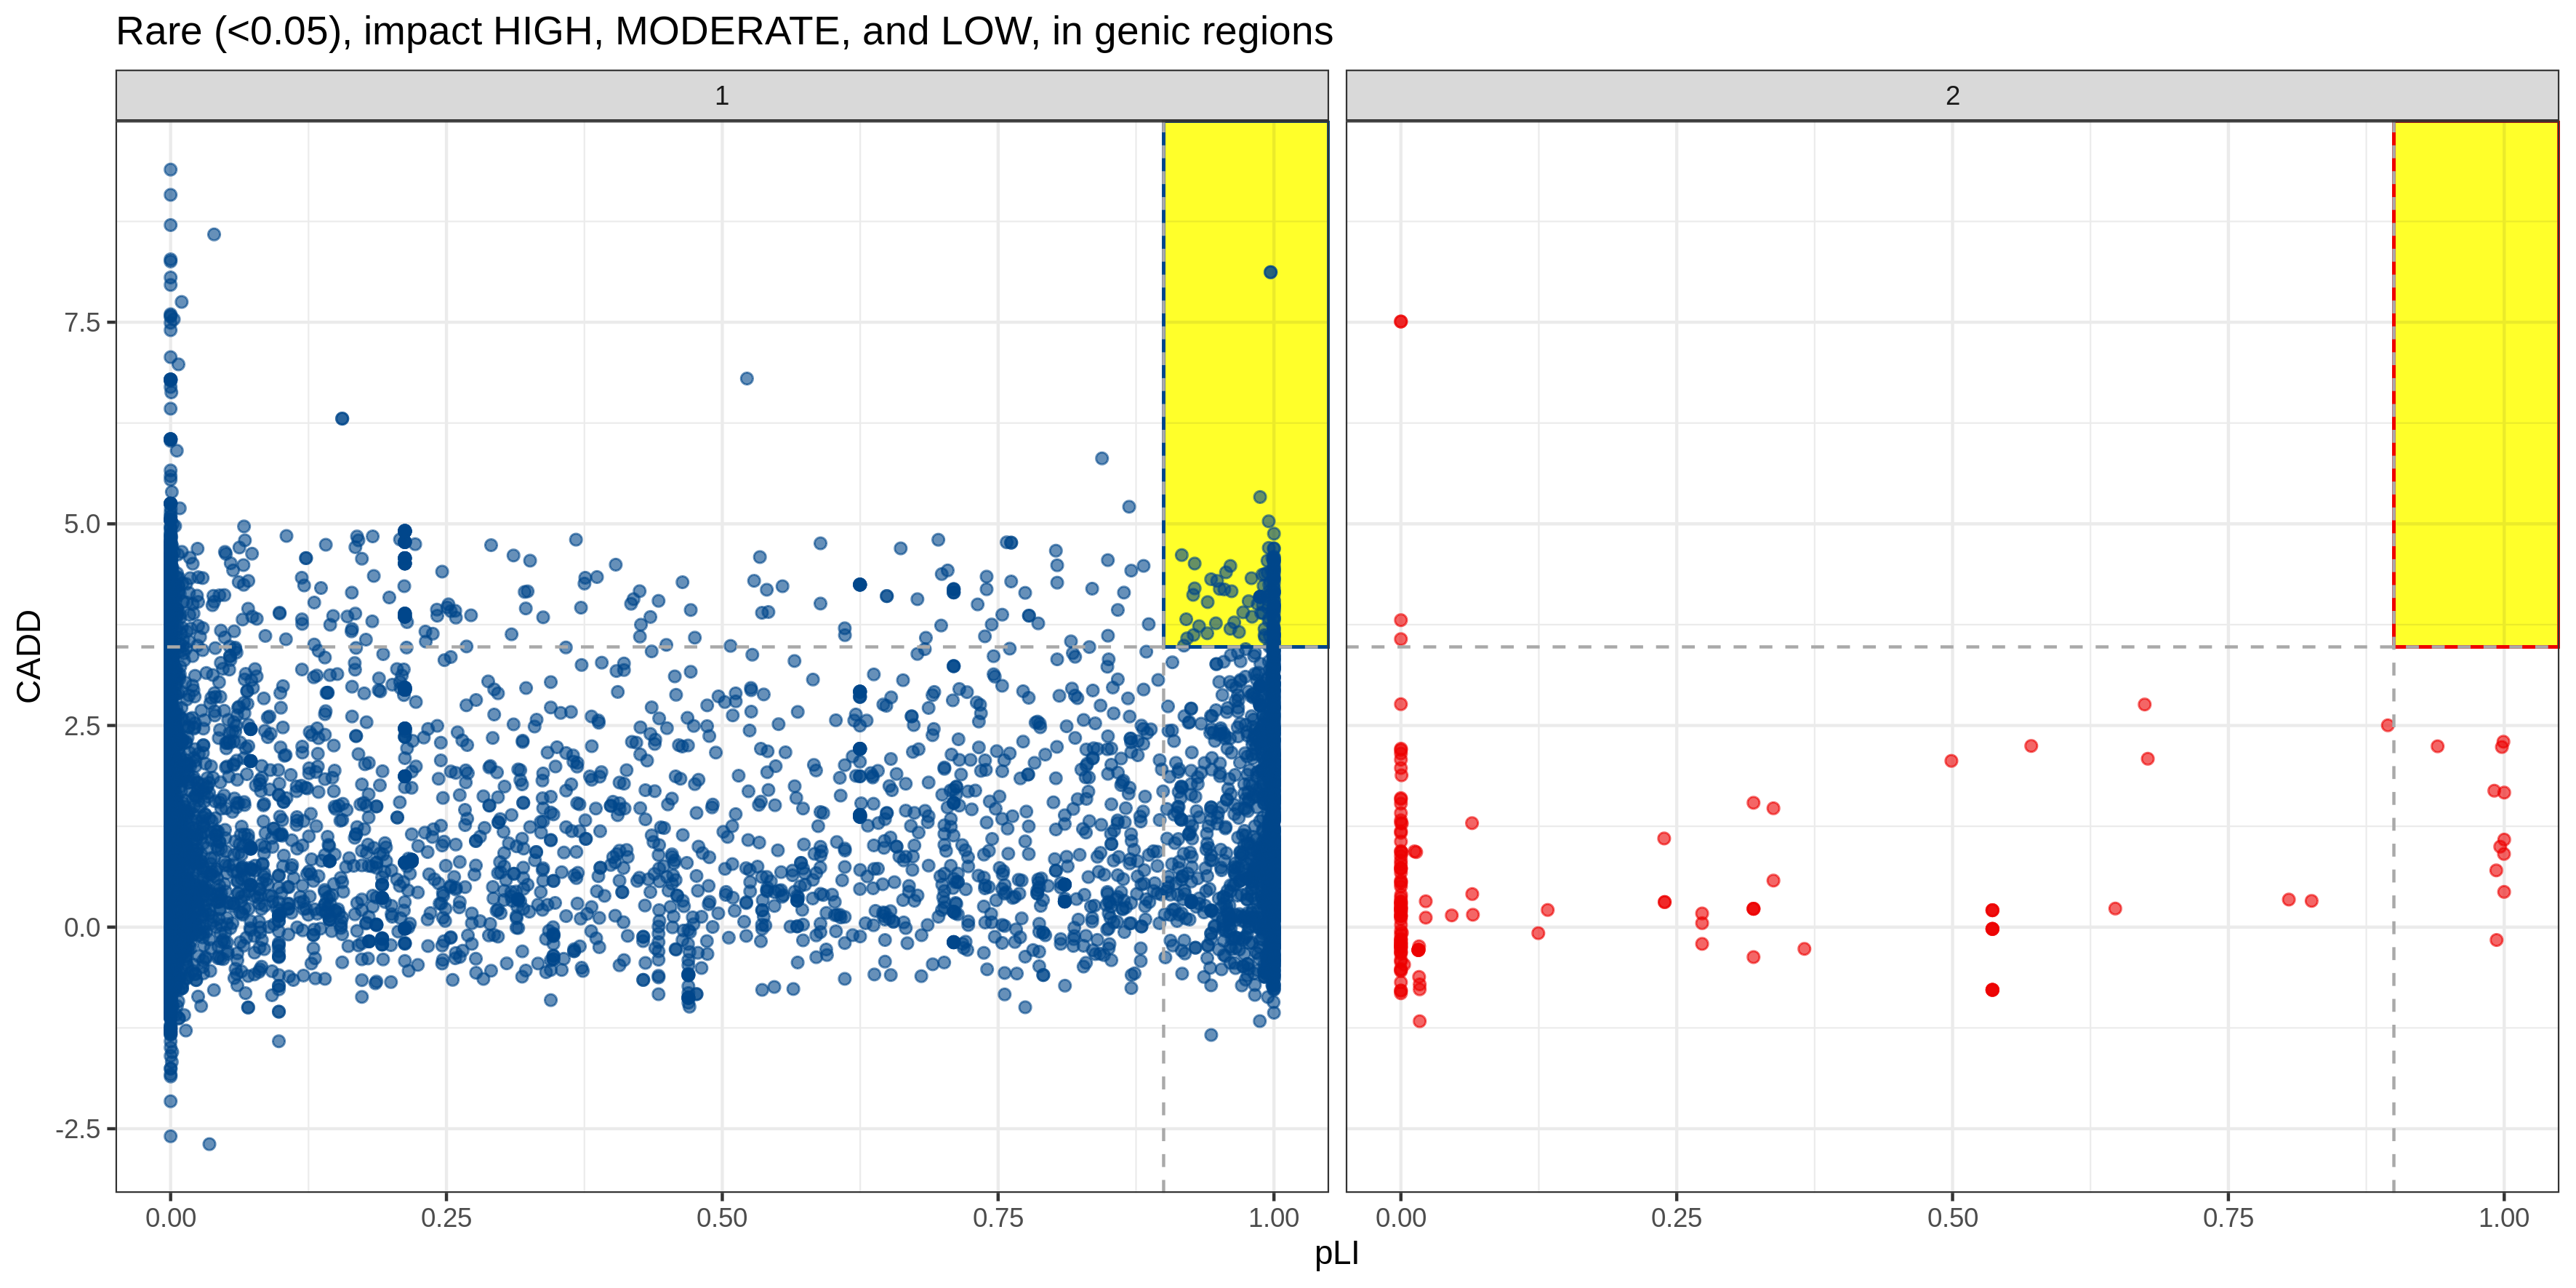
\includegraphics[width=1\textwidth]{fig/filter2py.png}
\decoRule
\caption{\textbf{Variants with high CADD and pLI.}}
\label{fig:filter2output}
\end{figure}

\subsubsection{Genes hosting filtered variants }
I aggregated the filtered variants in genes and calculated how many samples share variants in the same gene. The majority of genes are selected in only one  individual, while eleven genes are shared among two or more individuals  (Figure \ref{fig:geneCADDpLI}).\\

\vspace{1,5cm}

\begin{figure}[H]
\centering
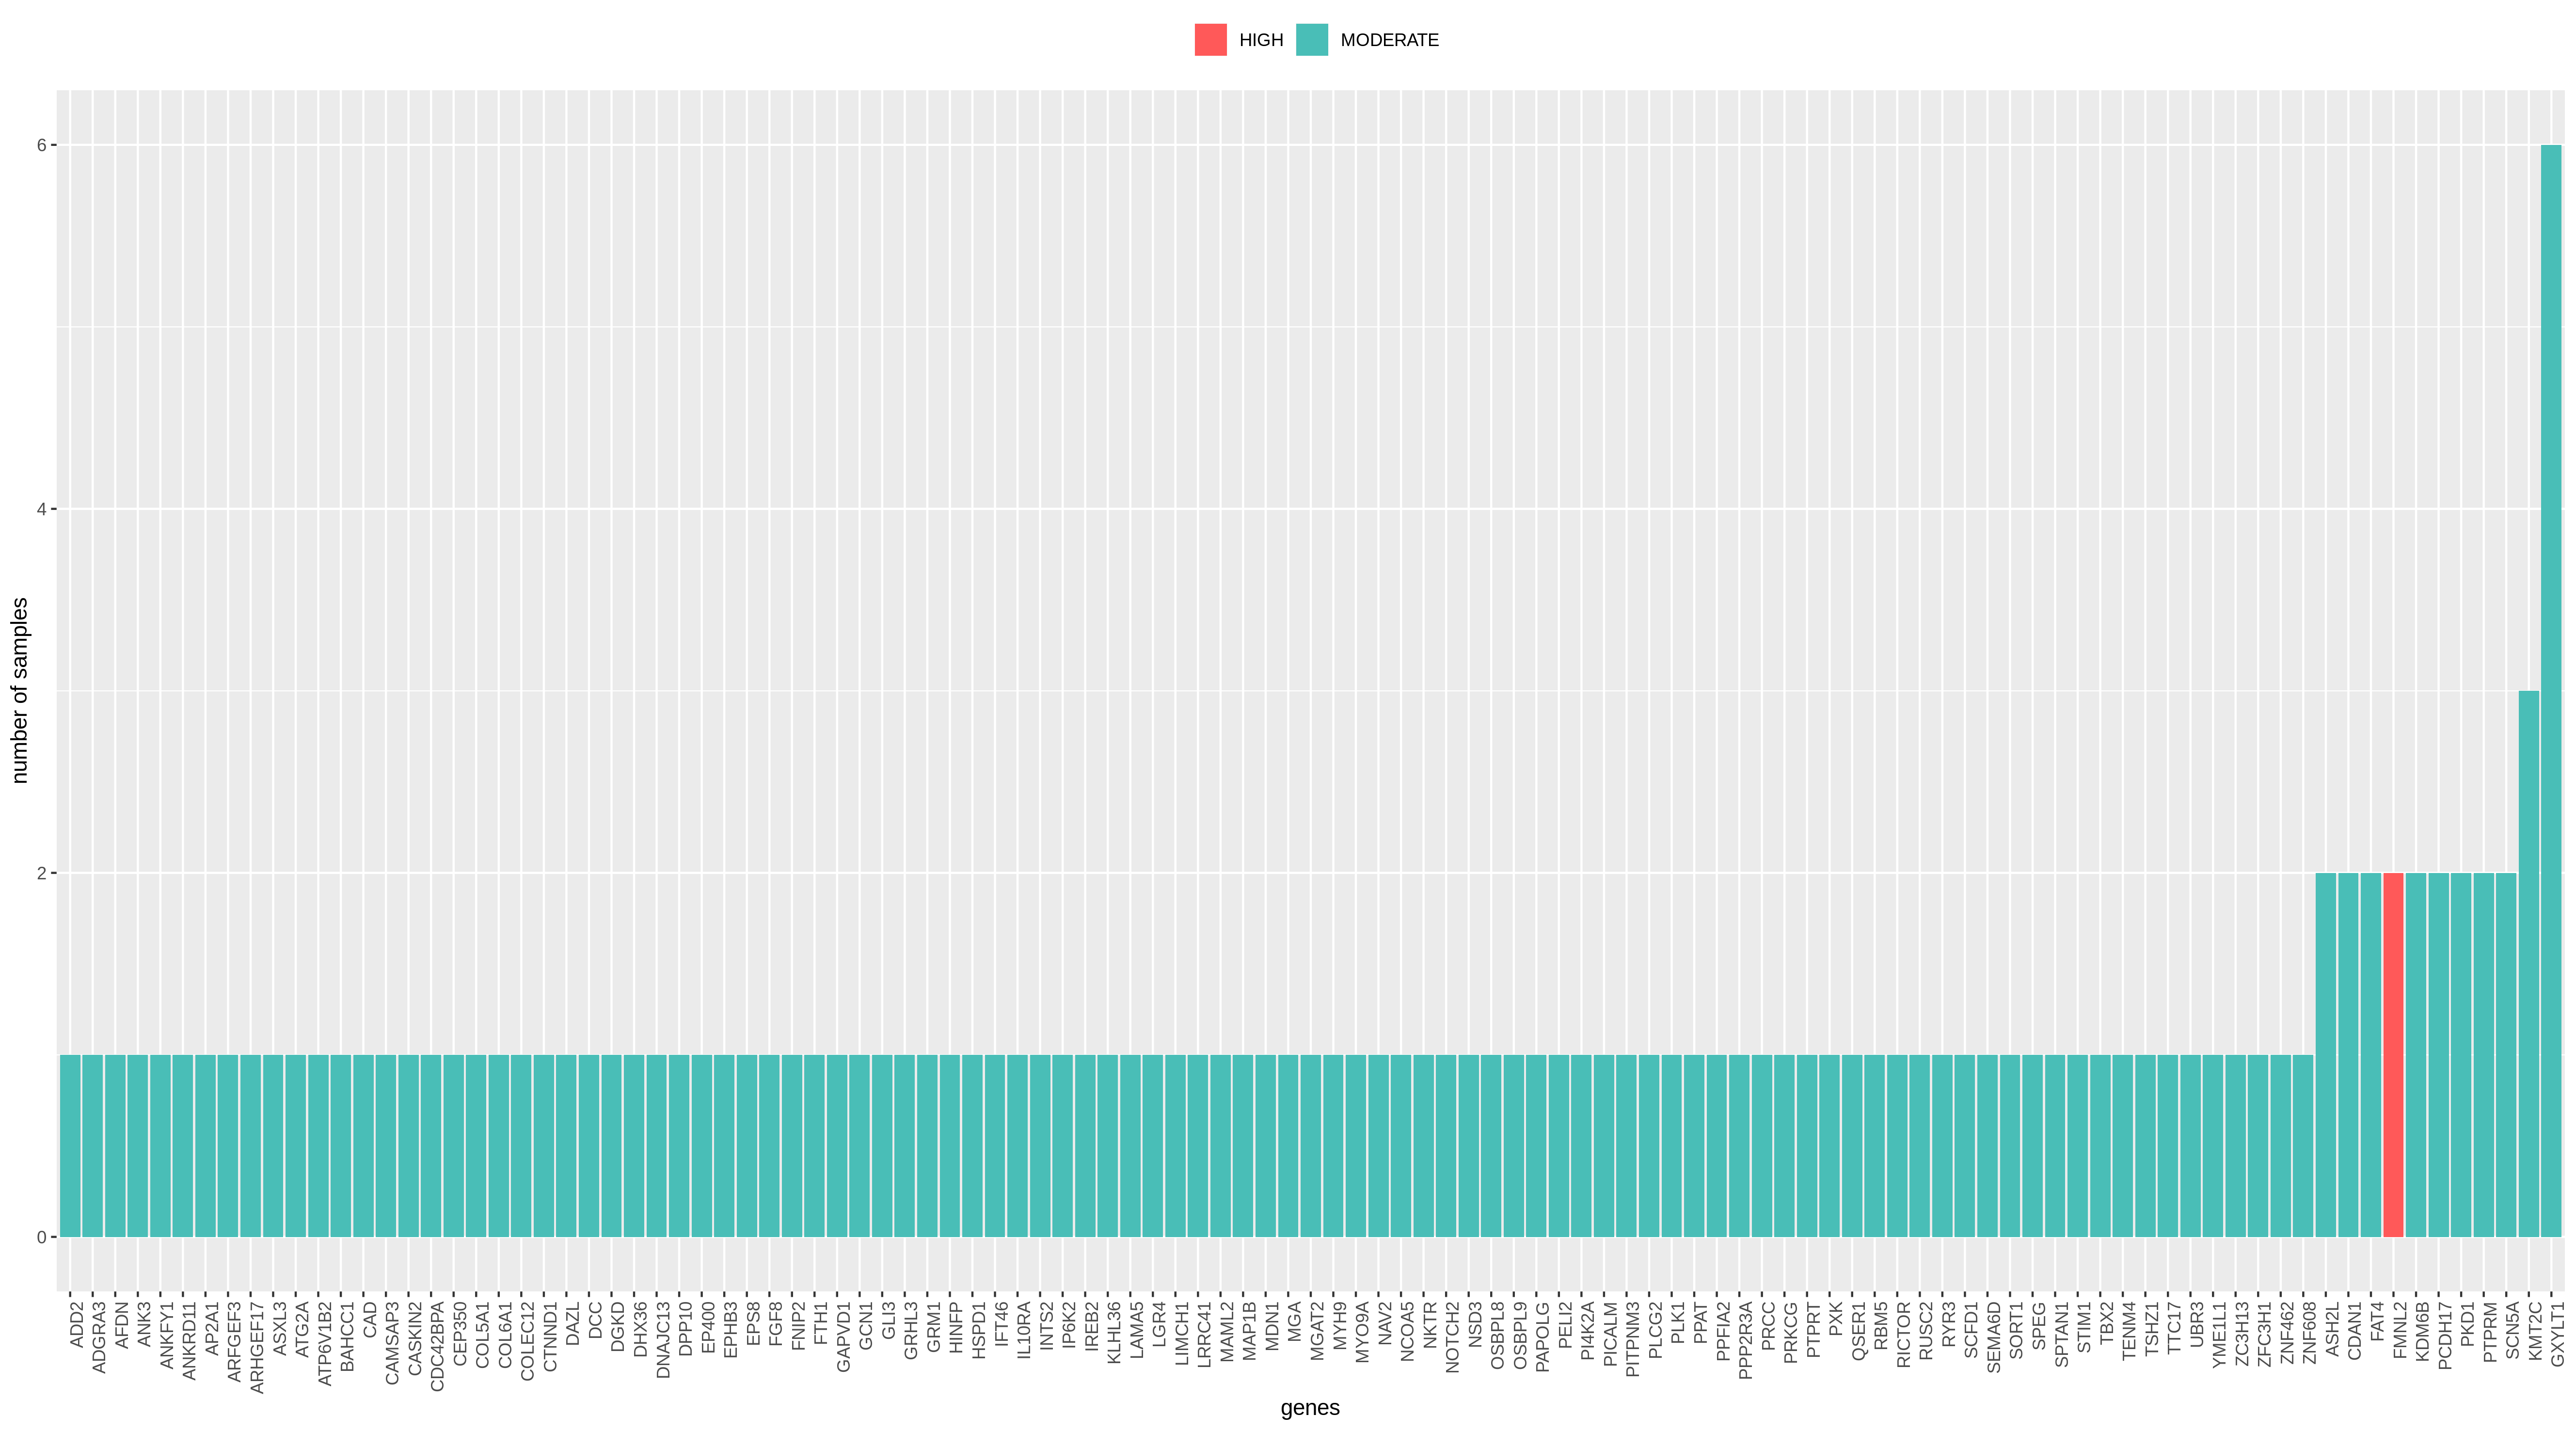
\includegraphics[width=1\textwidth]{fig/all_hetero_cadd_pli.png}
\decoRule
\caption{\textbf{Gene with high CADD and pLI.}}
\label{fig:geneCADDpLI}
\end{figure}

\vspace{1cm}

One \textbf{high impact} variant (rs750755379) that cause a Glu>Stop change in the protein is located in the sixth exon of the \textit{FMNL2} gene and is shared by two samples (Figure \ref{fig:fmnl2}). \textit{FMNL2} (ENSG00000157827) codes for a formin-related protein and has 4 transcripts (splice variants), 256 orthologues, 18 paralogues. It is located on chromosome 2:152,335,174-152,649,826 forward strand. Formin-related proteins have been implicated in morphogenesis, cytokinesis, and cell polarity. \textit{FMNL2}, in particular, is expressed in the fetus in the cytoplasm of brain, spinal cord, and rectum\cite{lizio2015gateways}. It is implicated in cytoskeleton organization (GO:0007010), regulation of cell shape (GO:0008360), cellular component organization (GO:0016043), cell migration (GO:0016477), regulation of cell morphogenesis (GO:0022604), actin cytoskeleton organization (GO:0030036), cortical actin cytoskeleton organization (GO:0030866). \\

\begin{figure}[H]
\centering
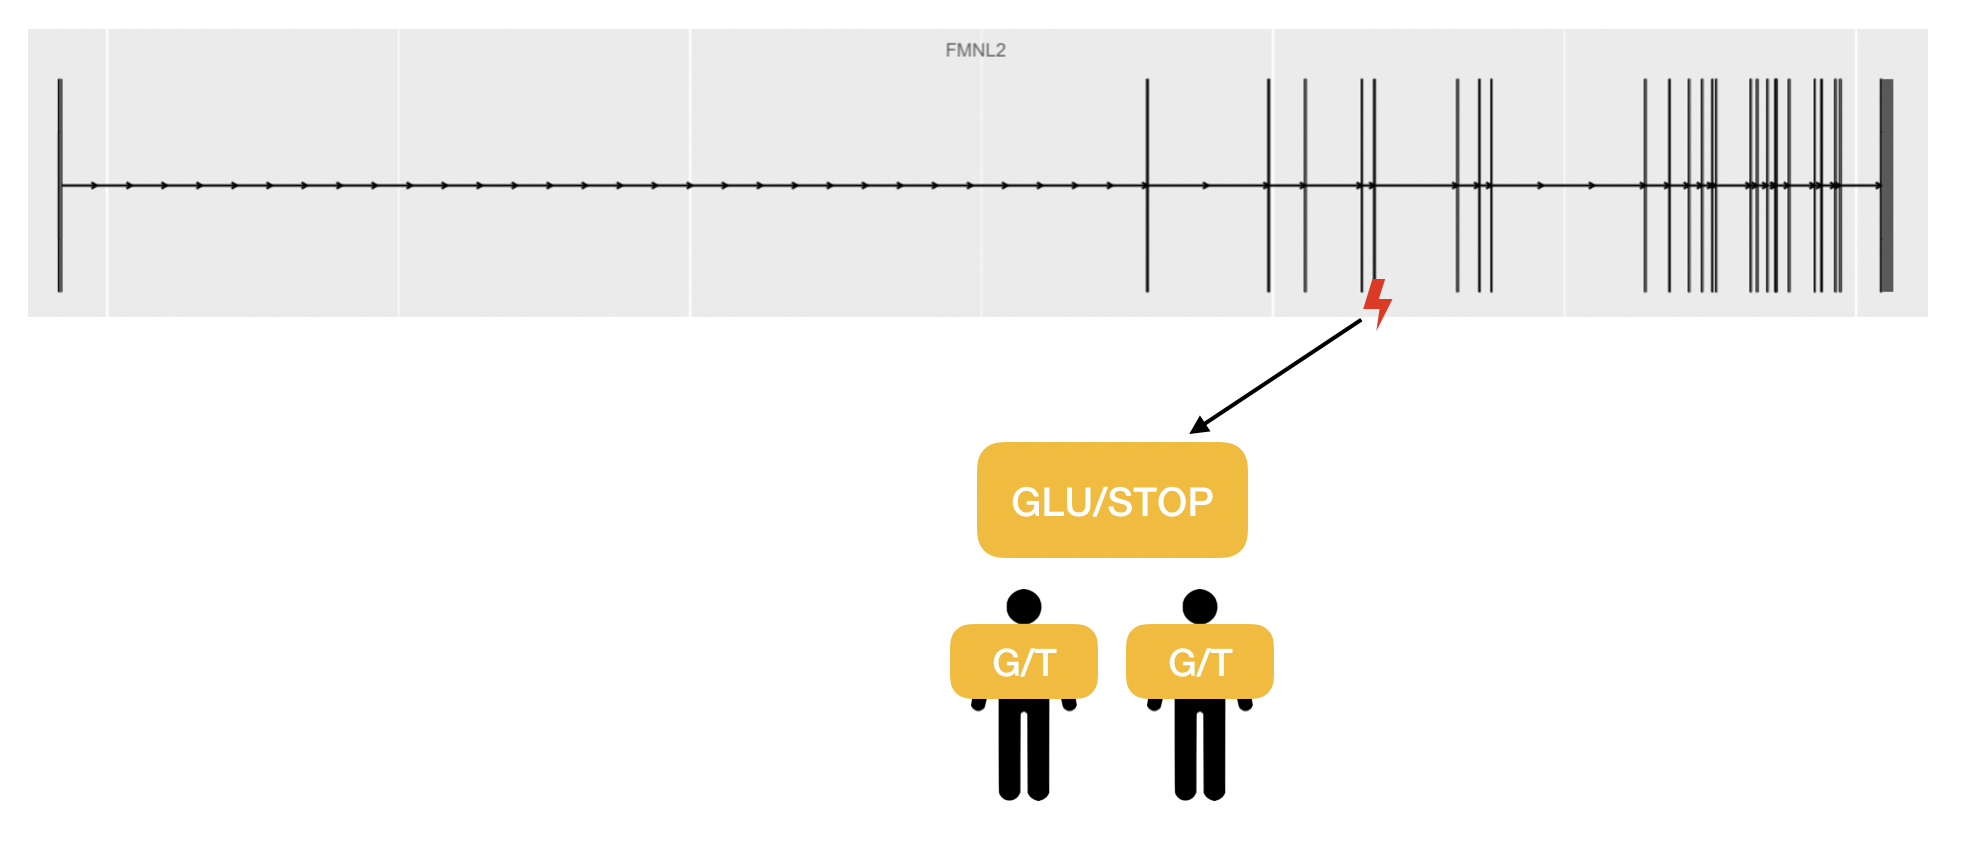
\includegraphics[width=0.95\textwidth]{fig/FMNL2_structure.png}
\decoRule
\caption{\textbf{Stop gained mutation in \textit{FMNL2} shared by two samples.} In the fetus \textit{FMNL2} is expressed cytoplasm of brain, spinal cord, and rectum where it is involved in cytoskeleton organization}
\label{fig:fmnl2}
\end{figure}

Among variants with \textbf{moderate impact}, the missense variant (rs78540738) in the fifth exone of the \textit{GXYLT1} gene is shared among all samples (Figure \ref{fig:gxylt1}). \textit{GXYLT1} is a glucoside xylosyltransferase with 2 transcripts (splice variants), 328 orthologues, 5 paralogues, located on chromosome 12: 42,081,845-42,144,874 reverse strand. The protein is a trans-membrane protein and the rs78540738 mutation corresponds to an Asp>Tyr change in the extra-cellular domain of the protein. \textit{GXYLT1} is implicated in the O-linked glycosylation\cite{sethi2010identification}, i.e. the attachment of a sugar molecule to the oxygen atom of serine (Ser) or threonine (Thr) residues in a protein.\\

\begin{figure}[H]
\centering
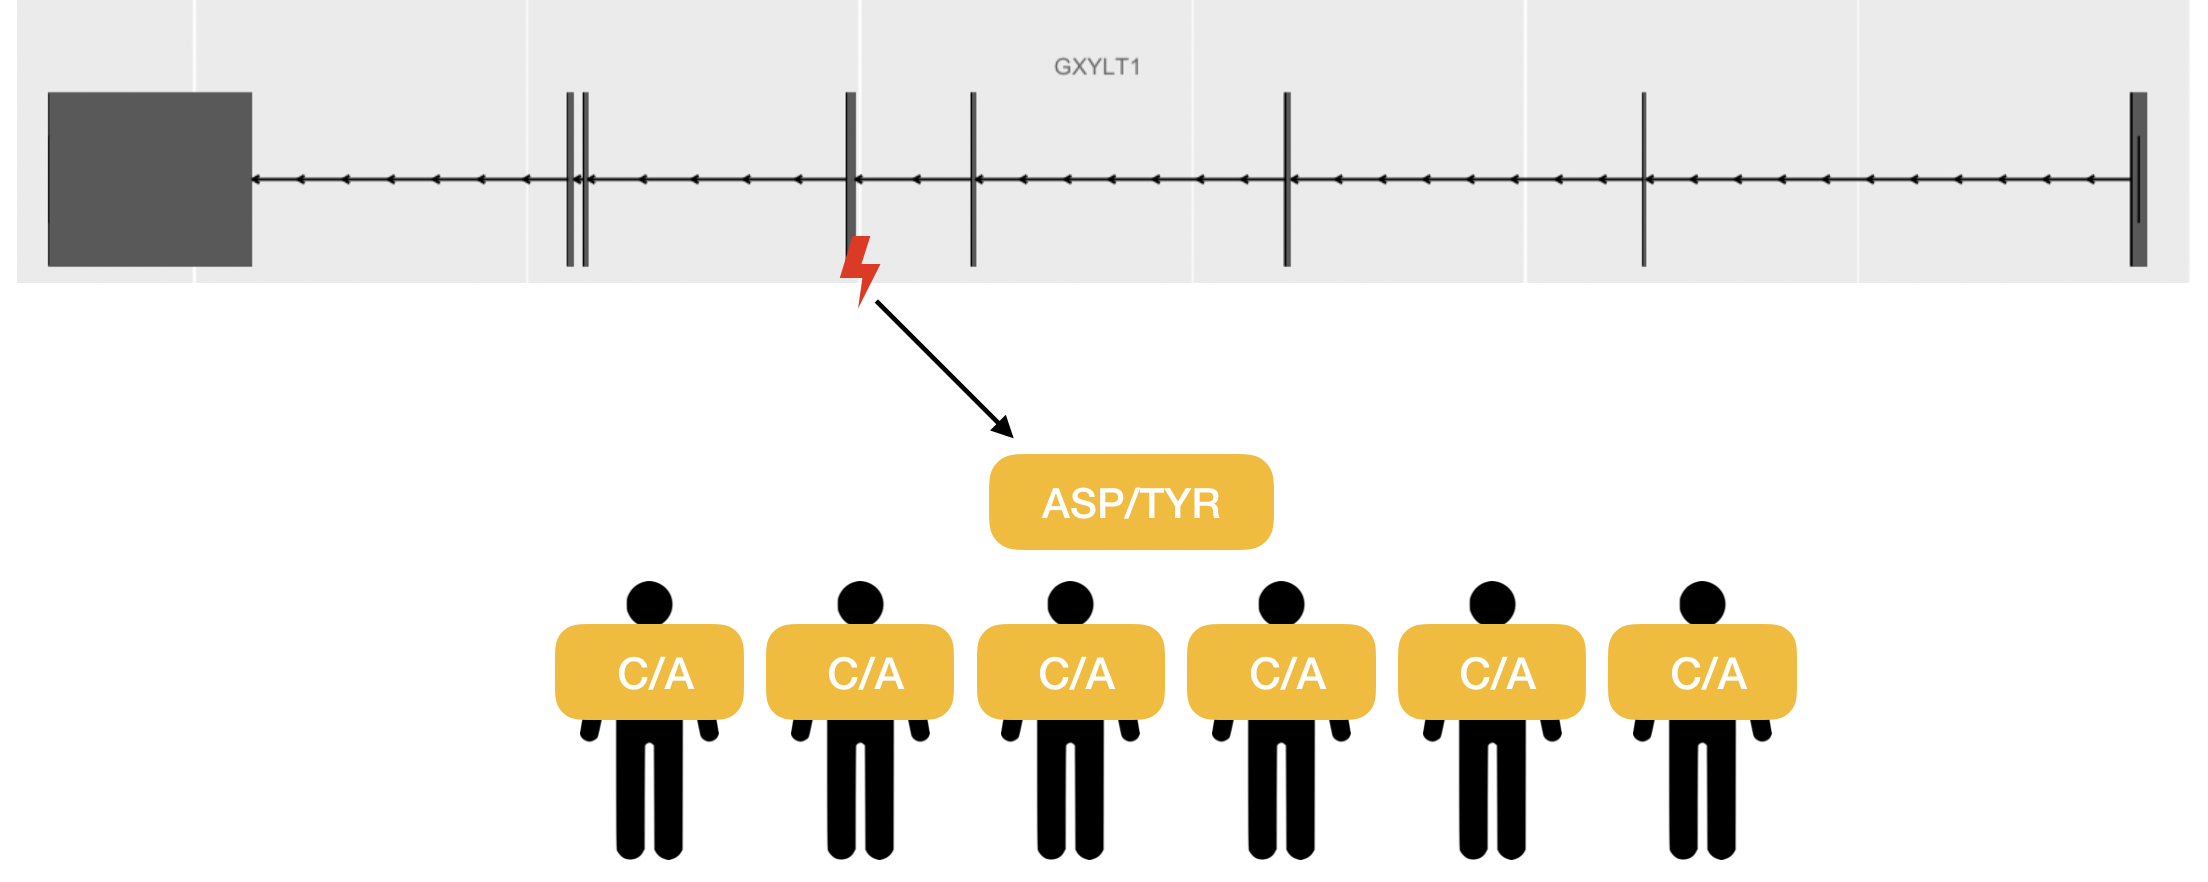
\includegraphics[width=0.95\textwidth]{fig/GXYLT1_structure.png}
\decoRule
\caption{\textbf{Missense mutation shared by all the six samples in the \textit{GXYLT1} gene.} The gene has two transcripts. The mutation we identified is rare in the general population (less than 0.01\%). \textit{GXYLT1} is a transmembrane protein. The mutation shown here corresponds  to  an  Asp>Tyr  change  in the extra-cellular domain of the protein.} 
\label{fig:gxylt1}
\end{figure}

\subsubsection{Integration of gene lists information}
To further reduce the number of genes, I integrated the information on gene lists by constraining for the variant to be in a gene that is present in at least two lists of relevant genes. The addition of this further filtering criteria, yields a list of twenty-two missense variants on average more deleterious (average CADD = 4.27) compared to previosly identified variants, located in twenty-two genes highly intolerant to loss of function (average pLI = 0.99). \\ 



%\todo{manca questa tabella, la ha silvia?}

{\small
\begin{table}
\caption{Expression level of LAMA5 in RIKEN FANTOM5 project}
\label{tab:lama5Exp}
\centering
\begin{adjustbox}{width=0.9\textwidth}
\begin{tabular}{1 1 1 1 1 1 1 1}
\toprule
\tabhead{Gene} & \tabhead{Colon} & \tabhead{Duodenum} & \tabhead{Lung} & \tabhead{Parietal lobe}  & \tabhead{Thyroid gland} & \tabhead{Umbilical cord} & \tabhead{Zone of skin}\\
\midrule
LAMA5 & 0.6 & 0.9 & 1.0 & 0.5 & 0.6 & 2.0 & 2.0 \\
\bottomrule
\end{tabular}
\end{adjustbox}
\end{table}
}

Among these genes, four samples have multiple heterozygous missense substitutions at seven sites in the \textit{LAMA5} gene (Figure \ref{fig:lama5}), located on the reverse strand of chromosome 20 in position 62,307,955-62,367,312. \textit{LAMA5} is a 59kb long gene composed of 80 exons. It has 14 transcripts (splice variants), 216 orthologues, and 28 paralogues. One of the missense mutations (rs78026347) has CADD score above the 90 percentile and cause a Pro>Leu of the 317th residue of the protein, located in a disulfide bond.
\textit{LAMA5} is a gene involved in the embryo development (GO:0009790). Mutations in \textit{LAMA5} have been associated to miscarriages \cite{laisk2019genetic,pereza2017systematic,qiao2016whole,rull2012genetics,colley2019potential,quintero2017novel} and are are lethal at early embryonic stages \cite{dawes2019gene}. It regulates the attachment, migration, and organization of cells into tissues during embryonic development. During fetal development, \textit{LAMA5} is highly expressed in the umbilical cord and in the skin (Table \ref{tab:lama5Exp})\cite{noguchi2017fantom5}.\\ 
In vertebrates, \textit{LAMA5} encodes for an alpha chain of the \textit{Laminins}\cite{aumailley2013laminin}, extracellular matrix glycoproteins composed by three non-identical multidomain chains (alpha, beta, and gamma) encoded by different genes that form a cruciform structure with one chain for each arm. \textit{Laminins} are the major noncollagenous constituent of basement membranes that are involved in cell adhesion and other different biological processes.

\begin{figure}[H]
\centering
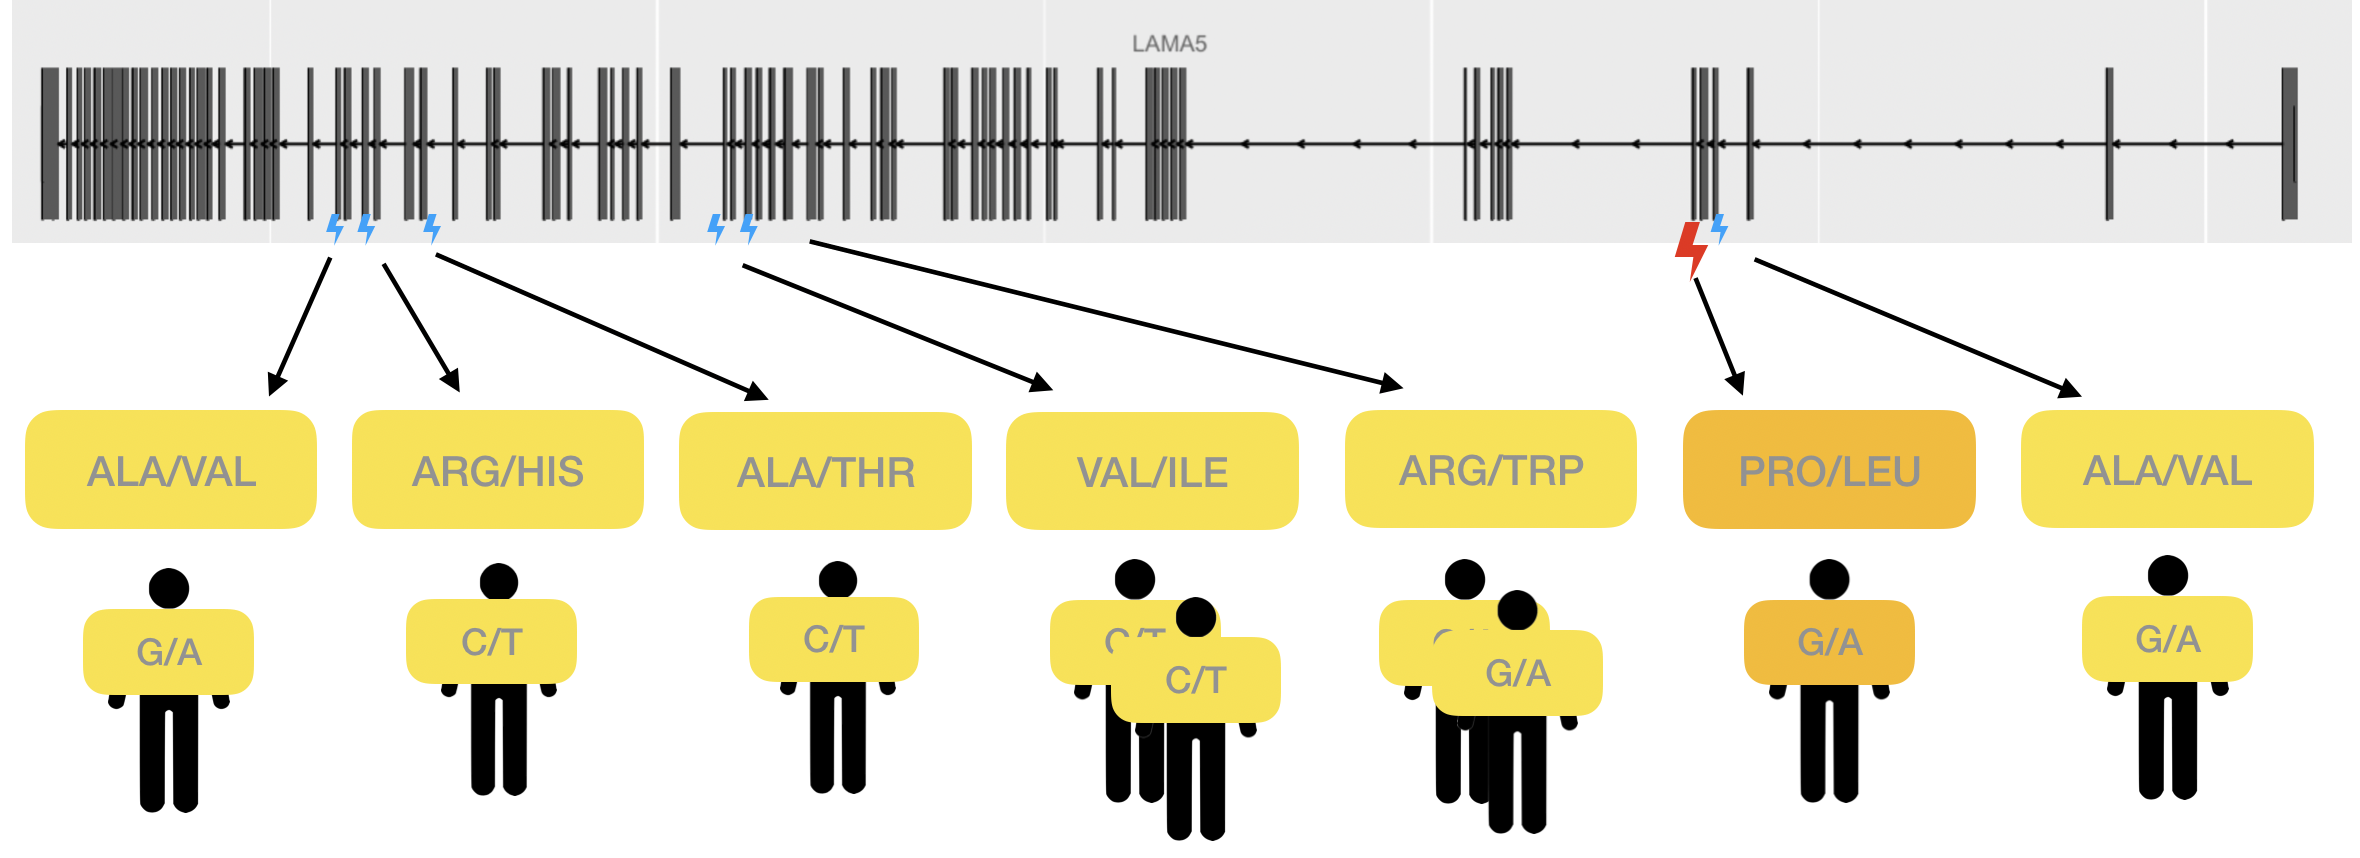
\includegraphics[width=0.95\textwidth]{fig/LAMA5_structure.png}
\decoRule
\caption{\textbf{Missense mutations in the \textit{LAMA5} gene}. \textit{LAMA5} is a gene involved in the embryo development (GO:0009790). Mutations in \textit{LAMA5} have been associated to miscarriages \cite{laisk2019genetic,pereza2017systematic,qiao2016whole,rull2012genetics,colley2019potential,quintero2017novel} and are are lethal at early embryonic stages \cite{dawes2019gene},  and in fact its pLI score is 0.94. It regulates the attachment, migration, and organization of cells into tissues during embryonic development. One of the missense mutations(dark orange) has CADD score above the 90 percentile.} 
\label{fig:lama5}
\end{figure}


% Chapter discussion

\chapter{Discussion} % Main chapter title

\label{Chapter4} % For referencing the chapter elsewhere, use \ref{Chapter4} 

%----------------------------------------------------------------------------------------

% Define some commands to keep the formatting separated from the content 
\newcommand{\keyword}[1]{\textbf{#1}}
\newcommand{\tabhead}[1]{\textbf{#1}}
\newcommand{\code}[1]{\texttt{#1}}
\newcommand{\file}[1]{\texttt{\bfseries#1}}
\newcommand{\option}[1]{\texttt{\itshape#1}}

%~~~~~~~~~~~~~~~~~~~~~~~~~~~~~~~~~~~~~~~~~~~~~~~~~~~~~~~~~~~~~~~~~~~~~~~~~~~~~~~~~~~~~~~

%~~~~~~~~ RE ANSWER

The genetic causes of pregnancy loss are not yet entirely understood. Current efforts target variants of large size or in coding regions, leaving unexplored a large fraction of the genome. Whit this work I demonstrated that it is possible to identify variants likely to cause idiopathic pregnancy losses using high-coverage whole-genome sequence data.\\ 

I analyzed genomic sequences of forty-four embryos from mothers that experienced pregnancy loss. From the analysis of available anthropometric and medical information we do not see any significant difference with a reference set of mothers that did voluntary termination of pregnancy, except for the significantly higher age of mothers presenting recurrent pregnancy loss. 

When screened with available diagnostic tools, about 70\% of the analyzed embryos present chromosome aneuploidies, as expected in the general population \cite{goddijn2000genetic,zhang2009genetic}. In this work I focused on the remaining 30\% apparently euploid for which whole-genome sequencing was performed. Knowing that roughly 30\% of the sample is sequentiable allows to calculate the overall number of samples to collect, given the number of samples to sequence to scale the project.   

I analyzed genome sequences to discover roughly 4.7M genomic variants per individual, as expected for a Human genome \cite{1000genome2015global}. Using a filtering procedure  based on genomic annotations and on the hypothesis that miscarriage is a complex polygenic trait, I identified several variants that are likely to be deleterious and therefore putatively causative. For each sample, the filter starts from millions of variants to obtain less than fifty variants per sample located in 112 genes. I further report on three genes either because they are shared among samples (\textit{FMNL2}, and \textit{GXYLT1}) or because they are lethal (\textit{LAMA5}). \textit{FMNL2}, and \textit{LAMA5} are involved in attachment, migration and organization of cells into tissue during embryonic development. \textit{GXYLT1}, is involved on the O-glycosilation.\\

We did not expect major overlaps among samples, as we expected that each case is due to a different set of mutations. Nevertheless, it was encouraging to find overlaps already with this small data set. Furthermore, while this study find candidates for causative mutations, it also suggests possible improvements. The filter that I used  seems to be quite stringent as it identifies a very limited number of variants, therefore it can be relaxed or based on a more effective combination of parameters. Also, it would be useful to develop a strategy to evaluate false positives and negatives. Finally, in the cases with multiple deleterious variants in heterozygosis it would be informative to reconstruct the phase of the variants to understand if both  if both copies of the genes are compromised.\\ 


Compared to what already available in literature \cite{laisk2019genetic,qiao2016whole,fu2018whole}, this project uses a novel approach for the study of the genetic causes of miscarriages, i.e. it looks at whole-genome. While here I present results for the coding part of genome, the GREP group is working to include regulatory and intergenic regions, therefore providing a complete scan of the genome. These first results will be corroborated with a more comprehensive analysis that fully implements a predictive model and includes regulatory regions.\\


Overall, I demonstrated that whole-genome sequencing can help to clarify part of the causes of pregnancy loss and provides essential indications for the realization of a larger study.



%For answer at this questions we have done a preliminary study on the medical data on the mothers. This kind of analysis is essential for future sampling for miscarriages, helping us to rule out some medical data such as BMI (Figure \ref{fig:panel_BMI_MenAge}.B) and suggest taking note of the length of the fetus when spontaneous abortion is diagnosed because the weeks are not informative and it is possible that the abortion occurred earlier \todo{we demonstrate that our data set complies to the standard}. After this explorative analysis from 119 samples only 29\% can be sequenced, this data is important for estimate the number of samples that we have to collect for having about one thousand sequences (Figure \ref{fig:pipelineOutcome}). With pre-sequencing screening for aneuploidies we have that trisomy of chromosome 22 is the most shared in our samples because an embryo with other trisomies can't arrive at the stage of 8-12 weeks but is development is arrested in an early stage (Figure \ref{fig:preseqOutcome}).\\

%After the sequencing the bioinformatics analysis and data obtained by \textsc{VEP} reveals no macroscopic differences between genomics sequence, the cause may be searched in SNPs or CNVs. Therefore we are interested in developing this software to discover these still unknown causes.\\




%The novelties of this study was the analysis of embyo's DNA for a whole-genome analysis. The focus was moved to SNPs, and CNVs in all DNA regions and not only in the exome as done to date.

% parlare dell'approccio innovativo di uno script che metta insieme più cose riguardanti i miscarriages (liste di geni associati, score CADD e pLI) e restituisca dei geni candidati che possono essere usati per fare esperimenti in vivo


%~~~~~~~~~~~~~~~~~~~~~~~~~~~~~~~~~~~~~~~~~~~~~~~~~~~~~~~~~~~~~~~~~~~~~~~~
%After the analysis with VEP, we have filtered from 4.5 Million variants, for each sample, to 1 Million of variants that have consequences on phenotype.


%This thesis has been a pilot for the project in my lab.
%Each point that has been analyzed in the results is needed for us to outline the future step for this project.\\

%Analysis of medical data is essential for future sampling for miscarriages.
%Helping us to rule out some medical data such as BMI (Figure \ref{fig:bmi}) and suggest taking note of the length of the fetus when spontaneous abortion is diagnosed because the weeks are not informative and it is possible that the abortion occurred earlier.\\

%From 119 samples only about 20\% go to sequencing, and this is important to understand the number of samples for having about 1000 sequences and do population analysis (Figure \ref{fig:pipeline_screening}).\\

%Referring to aneuploidies, trisomy of chromosome 22 is the most shared in our samples because an embryo with other trisomies can't arrive at the stage of 8-12 weeks but is development is arrested in an early stage (Figure \ref{fig:aneuploidies_CHG}).\\

%The data extracts from VEP software are complex and huge, the example in Figure \ref{fig:vep_example_output} is for each site of each chromosome that differs from the reference at least in one allele.
%The amount of data is so large that it forces us to work on a  server for handling.\\

%The summary results after VEP are interesting for us to understand if there is a macroscopic difference with normal data and at this point, we can assume that there isn't this kind of difference but the cause may be searched in SNPs or CNVs. 
%Therefore we are interested in developing this software to discover these still unknown causes.\\

%The software is still in development and in a short time, we will complete the first version that makes an additive score for prioritize each site and give us a complex score built around parameters that we choose to use.\\

%The results of actual version of software are encouraging because we denote an overlapping in 3 samples of 6 and is in a gene that is correlated with miscarriage and cancer.
%\emph{AHNAK2} is a cytoplasmatic nucleoprotein of which little is known. It is probably not our "Golden Boy" but is a nice example that what we make is on the right way.


% Chapter methods

\chapter{Methods} % Main chapter title

\label{Chapter5} % For referencing the chapter elsewhere, use \ref{Chapter5} 

%----------------------------------------------------------------------------------------

% Define some commands to keep the formatting separated from the content 
\newcommand{\keyword}[1]{\textbf{#1}}
\newcommand{\tabhead}[1]{\textbf{#1}}
\newcommand{\code}[1]{\texttt{#1}}
\newcommand{\file}[1]{\texttt{\bfseries#1}}
\newcommand{\option}[1]{\texttt{\itshape#1}}

%~~~~~~~~~~~~~~~~~~~~~~~~~~~~~~~~~~~~~~~~~~~~~~~~~~~~~~~~~~~~~~~~~~~~~~~~~~~~~~~~~~~~~~~






\section{Data and sample collection.} Study material consisted in blood and embryos from the mothers and was collected at the Section Unit of Obstetrics and Gynecology at the University Hospital of Ferrara from 2016 to 2018. The study was approved by the ethical committee of the Emilia-Romagna (CE/FE170475 G.R Reg. E/R (PRUA1GR-2013 00000220 “Silent Intrauterine infections and early pregnancy loss”) and was carried out in compliance with the Helsinki Declaration. All participants provided written informed consents prior to recruitment. All patient data were anonymized right after data and sample collection.\\ 

Data were cleaned and refined (e.g.trimming of white spaces, correction of typing errors, harmonization of values within fields, and similar) using OpenRefine (\url{https://github.com/OpenRefine/OpenRefine}), a standalone open source application for data cleanup and transformation (\href{https://en.wikipedia.org/wiki/OpenRefine}{wiki}).\\

Summary statistics of the data and hypothesis testing were calculated and represented using the packages \textit{ggplot} \cite{ggplot2}, \textit{tidyverse} \cite{wickham2019welcome}, \textit{stats} \cite{statsR} and \textsc{r} \cite{R}. All the code is available on the git repository of the project (\url{https://github.com/ezcn/grep}) 

\section{Screening for chromosomal aneuploidies}

This part was performed by our collaborators at the University of Ferrara and Merigen Reserach s.r.l. In brief DNA was extracted from chorionic villi of the product of conception using standard protocols. A rapid screening of sex and numerical anomalies for chromosomes 13, 15, 16, 18, 21, 22 and X was carried out with the miscarriage DNA samples performing quantitative PCR assays. Samples that resulted euploid for these chromosomes were further analized by Comparative Genomic Hybridization (Agilent SurePrint G3) and low coverage sequencing of randomly amplified genomic regions


\section {Whole-genome sequence analyses}

\subsection{Sequencing}
Sequencing was done through a service provider (Macrogen s.r.l). In particular, libraries for sequencing were prepared using the Illumina TruSeq DNA PCR-free Library (insert size 350bp) and samples were sequenced at 30X mapped (~110Gb) 150bp PE on HiSeqX. Data were released in as fastq files. 

\subsection{Alignment with reference.} Reads in the fastq file were aligned against the reference genome GRChg38.p12 \cite{rosenbloom2015ucsc} using \textsc{bwa} and \textsc{samtools}. \textsc{bwa} (\url{https://github.com/lh3/bwa}) "is a software package for mapping low-divergent sequences against a large reference genome, such as the human genome." Of the three algorithms available in \textsc{bwa} we used \textsc{bwa-mem}  that is generally recommended to analyze 70-100bp Illumina reads.\\

Downstream to \textsc{bwa-mem} I used \textsc{samtools} (\url{https://github.com/samtools/samtools}) to obtain a BAM from a fastq. \textsc{samtools} "is a set of utilities for interacting with and post-processing short DNA sequence read alignments in the SAM (Sequence Alignment/Map), BAM (Binary Alignment/Map) and CRAM formats" (\href{https://en.wikipedia.org/wiki/SAMtools}{wiki}). 

For each sample, the following command line takes in input fastq file (paired-end) and gives as output a raw-bam file that contains the alignment of the reads against the reference genome: 

\begin{verbatim}
~/bin/bwa mem -t 16 -R "@RG\tID:$idsample\tSM:$idsample" \
/mpbastudies3/IMMA/hg38/hg38.p12.fa \ 
/mpbastudies3/181113_Vincenza-Colonna/$namedir/$nameflgz1 \ 
/mpbastudies3/181113_Vincenza-Colonna/$namedir/$nameflgz2 | \ 
/mpba0/mpba-sw/samtools view -b - > \
/mpbastudies3/IMMA/samples/$idsample.raw.bam
\end{verbatim}


\subsection{Refining}
The  process of library preparation prior to sequencing can introduce artifacts such as PCR duplications. Although the type of library used for the sequencing of the GREP samples is PCR-free we checked for PCR duplicates using the function markdup of \textsc{sambamba}. As expected we did non find replicates. 

SAMbamba (\url{https://github.com/biod/sambamba}) \textit{"is a high performance highly parallel robust and fast tool (and library), written in the D programming language, for working with SAM and BAM files"}  (\href{https://github.com/biod/sambamba#introduction}{git}).

The command line takes as input a raw version of the BAM file for each sample and gives as output a BAM file without PCR duplicates:  

\begin{verbatim}
~/bin/sambamba markdup -t 8 -p  \
--tmpdir /scratch --overflow-list-size 500000 \
/mpbastudies3/IMMA/samples/${idflrbam}.raw.sorted.bam \
/mpbastudies3/IMMA/samples/${idflrbam}.bam    
\end{verbatim}


\subsection{Variant calling} 
The variant calling identifies sites of an individual genome that differ from the reference sequence. We used \textsc{freebayes} (\url{https://github.com/ekg/freebayes}) that is "a Bayesian genetic variant detector designed to find small polymorphisms, specifically SNPs (single-nucleotide polymorphisms), indels (insertions and deletions), MNPs (multi-nucleotide polymorphisms), and complex events (composite insertion and substitution events) smaller than the length of a short-read sequencing alignment." (\href{https://github.com/ekg/freebayes}{git}).
\textsc{freebayes} requires the reference genome in fasta format and the BAM file for each sample. To speedup the process I did independent analysis for each chromosome for each individual. The command line that I used is: 

\begin{verbatim}
~/bin/freebayes -f /mpbastudies3/IMMA/hg38/hg38.p12.fa \ 
-r ${chr} --gvcf -g 2000  /mpbastudies3/IMMA/samples/${idsample}.bam 
\end{verbatim}

\subsection {Compress and indexing.} 
vcf files generated by \textsc{freebayes} are compressed and indexed. Compression optimizes files storage and transfer. Indexing allows fast access to large files. 

Compression was done using Bgzip (\url{https://www.htslib.org/doc/bgzip.html#DESCRIPTION}) that "compresses files into a series of small (less than 64K) 'BGZF' blocks. This allows indexes to be built against the compressed file and used to retrieve portions of the data without having to decompress the entire file" (\href{https://www.htslib.org/doc/bgzip.html#DESCRIPTION}{wiki}).
The command line takes in input the output (VCF) from variant calling and outputs the compressed file: 

\begin{verbatim}
~/bin/bgzip /mpbastudies3/IMMA/samples/vcf/${idsample}.vcf > \
/mpbastudies3/IMMA/samples/vcf/${idsample}.vcf.gz
\end{verbatim}

Indexing was done using Tabix (\url{https://www.htslib.org/doc/tabix.html}) that "indexes a TAB-delimited genome position file in.tab.bgz and creates an index file". The command line takes in input the compressed file from BGZIP and produces an indexed file: 

\begin{verbatim}
~/bin/tabix -p vcf /mpbastudies3/IMMA/samples/vcf/${id}.${chr}.vcf.gz 
\end{verbatim}


\subsection{Variant Effect Predictor.}  
VEP (\url{https://grch37.ensembl.org/info/docs/tools/vep/index.html}) determines the effect of genetic variants (SNPs, insertions, deletions, CNVs or structural variants) on genes, transcripts, and protein sequence, as well as regulatory regions. \textsc{vep} takes as input the coordinates of the variants and the nucleotide changes to find out the:
\begin{itemize}
    \item Alleles, Genes and Transcripts affected by the variants
    \item Location of the variants (e.g. upstream of a transcript, in coding sequence, in non-coding RNA, in regulatory regions)
    \item Consequence of the variation on the protein sequence (e.g. stop gained, missense, stop lost, frameshift)
    \item Matches with known variants, and associated  allele frequencies from databases of human sequences
    \item Several scores associated to changes to the protein sequence
\end{itemize}

\textsc{vep} takes in input a refined vcf file and gives as output an annotated vcf or a json file with information for all the parameters written in the command-line. I used the \textsc{vep} version 96.3 with the following command-line: 

\begin{verbatim}
singularity run -B /mpbastudies3/IMMA/samples/:/data \
/mpba0/mpba-sw/biocontainers/vep-96.3.img \
--af_1kg --af_gnomad --appris --biotype \
--buffer_size 5000 --check_existing --distance 5000 \
--fork 4 --polyphen b --pubmed --regulatory --sift b \
--species homo_sapiens --symbol --tsl --cache \
--dir_cache /mpba0/vcolonna/vepcache/ --offline \
--vcf --variant_class -i /data/vcfconcat/${id}.fullVcf \
-o /data/vepVCF/${id}.fullvep
\end{verbatim}

\subsection{Filtering and ranking using custom Python scripting}
    
\begin{figure}[H]
\centering
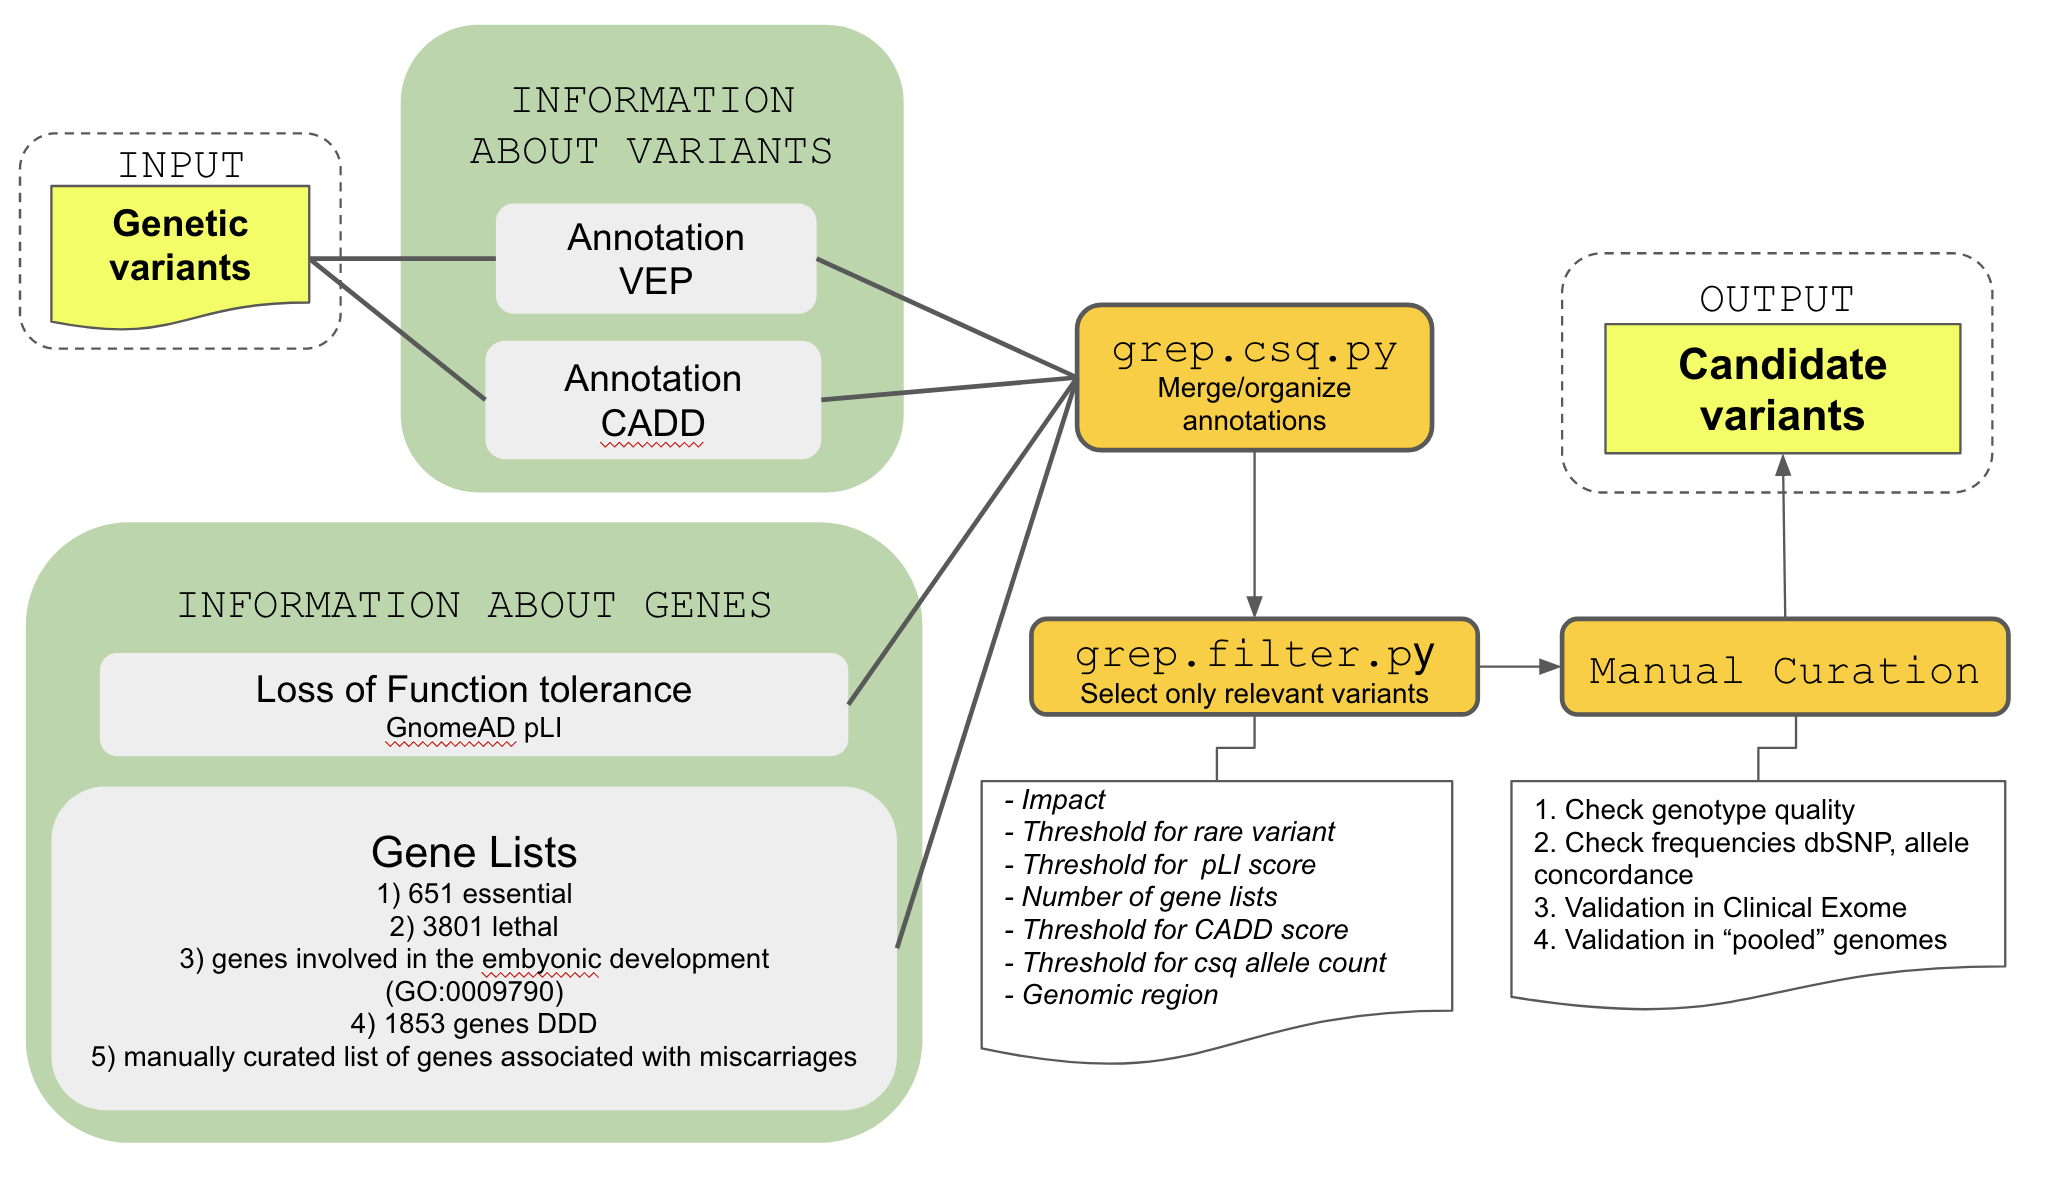
\includegraphics[width=0.95\textwidth]{fig/pipelineComplete.png}
\decoRule
\caption{\textbf{Our pipeline (\url{https://github.com/ezcn/grep})} is written in Python and in consists of two script. The first one (\textsc{grep.csq.py}) takes as input a file with the genomic location of the genetic variants and annotates it with the information from several databases on genetic variants and genes. The second (\textsc{grep.filter.py}) selects only relevant variants according to the filters specified by the user. The results of \textsc{grep.filter.py} are manually curated to obtain the candidate variants.} 
\label{fig:pipelineComplete}
\end{figure}


\subsection{Tools for High Performance Computing}

\subsubsection{Containers}
In the last few years the attention of programming world was moving to containers that are standard units of software that consist to package all the \gls{code} and \gls{dependencies} and allow to runs the packaged-software quickly and reliably from one computing environment to another. I have used two type of this containers, \textsc{singularity} \cite{kurtzer2017singularity} and \textsc{docker} \cite{merkel2014docker}. \textsc{singularity} have more flexibility than \textsc{docker} but defect stability and don't already have a big community of users and developers.

\subsubsection{Workload management systems}
All the analysis was made on remote HPC machine that use two software for parallelization of computationally intensive tasks \textsc{sgl} \cite{} and \textsc{htcondor}\cite{condor-practice}. \textsc{htcondor} was preferred to \textsc{sgl} for intensive and high computational tasks. \textsc{sgl} was used for simple and single core tasks.

\subsubsection{Programming languages}
I learned and used bash \cite{gnu2007free}, awk \cite{aho1979awk}, Python \cite{python3} 



%\printglossary

\printbibliography[heading=bibintoc]

\chapter{Conference Abstracts}
\begin{enumerate}
    \item Buonaiuto S. , Di Biase I. , Aleotti V. , \textbf{Damaggio G.} , D'Ambrosio P. , Catapano O. , Ravaei A. , Esposito G. , Chierici M. , Pulijala M. , Ayub Q. , Furlanello C. , Garrison E. , Soranzo N. , Capalbo A. , Rubini M. , Di Biase S. , Colonna V. . \textit{Deciphering genetic causes of idiopathic pregnancy loss from an embryonic perspective}. Biology of Genomes, Cold Spring Harbor Laboratory, US,2020\\

    \item Buonaiuto S. , Di Biase I. , Aleotti V. , \textbf{Damaggio G.} , D'Ambrosio P. , Catapano O. , Esposito G. , Chierici M. , Pulijala M. , Ayub Q. , Furlanello C. , Garrison E. , Soranzo N. , Capalbo A. , Rubini M. , Di Biase S. , Colonna V. . \textit{Identification of genomic variants responsible for pregnancy loss: a pilot study}. Network Tools and Applications in Biology /Bioinformatics and Computational Biology Conference, University of Fisciano, Italy - 2019\\

    \item Buonaiuto S. , Di Biase I. , Aleotti V. , Ravaei A. , \textbf{Damaggio G.} , D’Ambrosio P. , Catapano O. , Esposito G. , Chierici M. , Pulijala M. , Ayub Q. , Furlanello C. , Garrison E. , Soranzo N. , Capalbo A. , Rubini M. , Di Biase S. , and Colonna V. . \textit{Identification of genomic variants responsible for pregnancy loss: a pilot study}. European Society of Human Reproduction and Embryology 2020, Copenhagen, Denmark\\

    \item Kahraman S. , Sagir F. , Yuksel B. , Cetinkaya M. , Gavaz M. , Kara B. , Yesil M. , Akar G. , Buonaiuto S. , \textbf{Damaggio G. }, Fabiani M. , De Marino A. , Colonna V. , Simon C. , Capalbo A. . \textit {Genomics analysis of maternal exomes reveals new candidate genes and pathways for the diagnosis and prediction of recurrent preimplantation embryo arrest in IVF cycles}. European Society of Human Reproduction and Embryology 2020, Copenhagen, Denmark\\

    \item Buonaiuto S. , Di Biase I. , Aleotti V. , \textbf{Damaggio G.} , D'Ambrosio P. , Catapano O. , Esposito G. , Chierici M. , Pulijala M. , Ayub Q. , Furlanello C. , Garrison E. , Soranzo N. , Rubini M. , Di Biase S. , Colonna V. .  \textit{Genomics of Pregnancy Loss}. Associazione Genetica Italiana 2019, Cortona, Italy\\
\end{enumerate}

\begin{acknowledgements}
\addchaptertocentry{\acknowledgementname}
\end{acknowledgements}

\end{document}


